\chapter{Chapter 4. Results}

\renewcommand{\arraystretch}{0.9}

\section{Exploratory Model Runs}

As mentioned in the previous chapter, one of the main challenges encountered while training neural networks is the overwhelming number of independent variables that can affect model performance. These so-called ``hyperparameters'' may have complex interdependence, and there are few general best-practices. In order to identify a reasonable baseline for the performance of each of the model architectures, we started by training a wide variety of permutations on model properties including the number of layers, nodes per layer, activation function, and prediction coarseness, as well as training properties including loss function characteristics, batch normalization, and weight dropout rate. At this stage, developing a rigorous understanding of the effects of changes in model and training setup was not a priority; instead, we modified multiple hyperparameters simultaneously between training iterations with the goal of establishing rough rules of thumb and a sense for the approximate size of models needed for this task.

\begin{figure}[hp!]
    \centering
    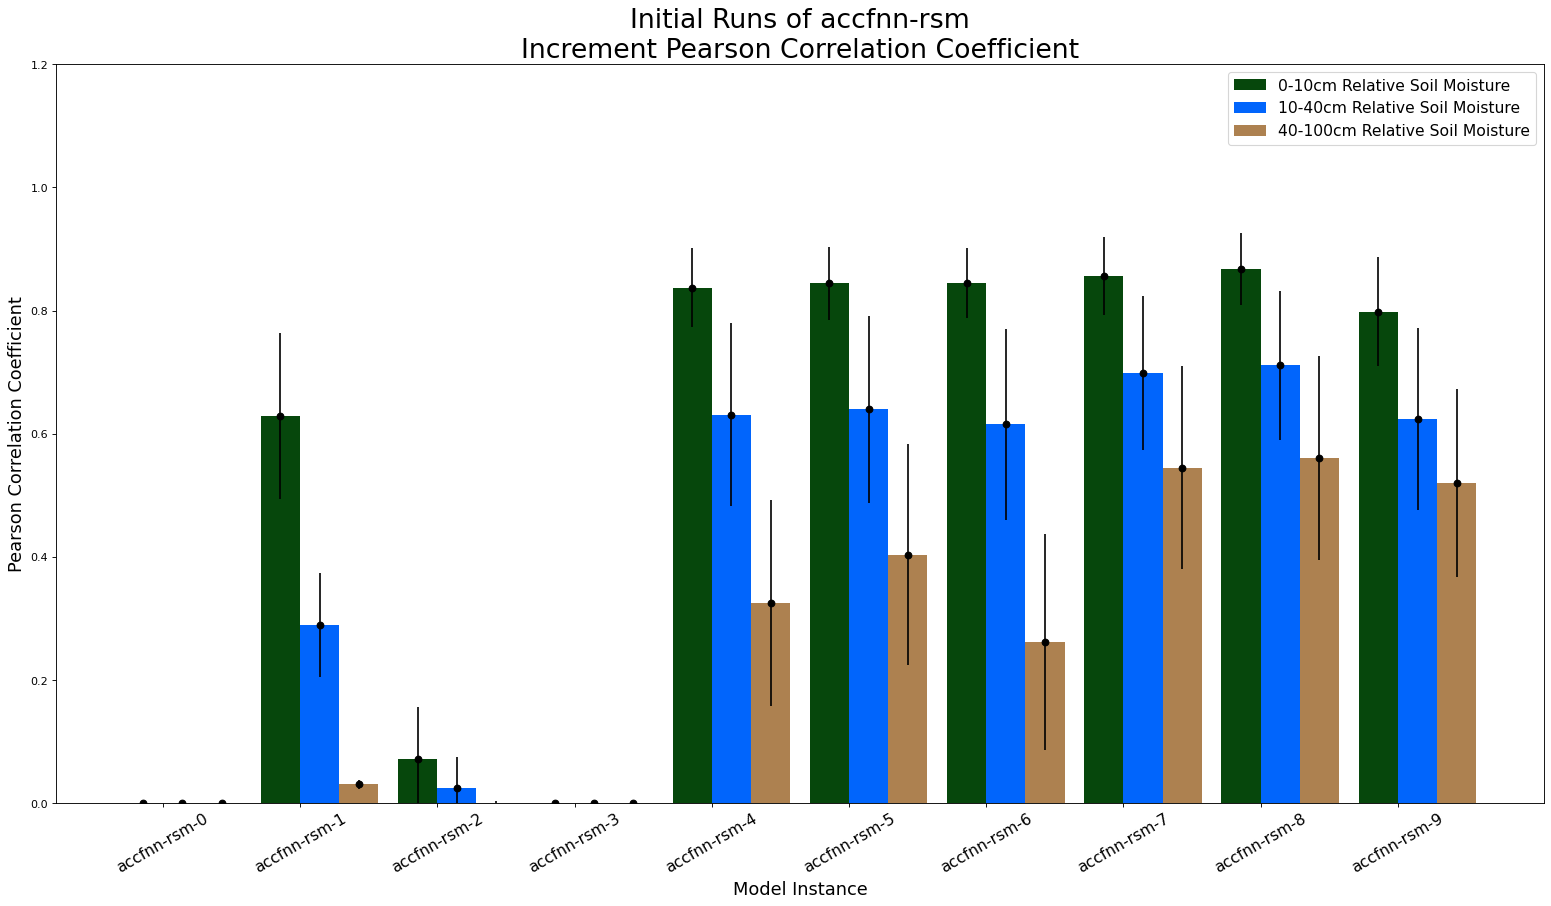
\includegraphics[width=.48\linewidth,draft=false]{figures/efficiency_initial-best/eval_test_efficiency_initial-accfnn-rsm_cc_res.png}
    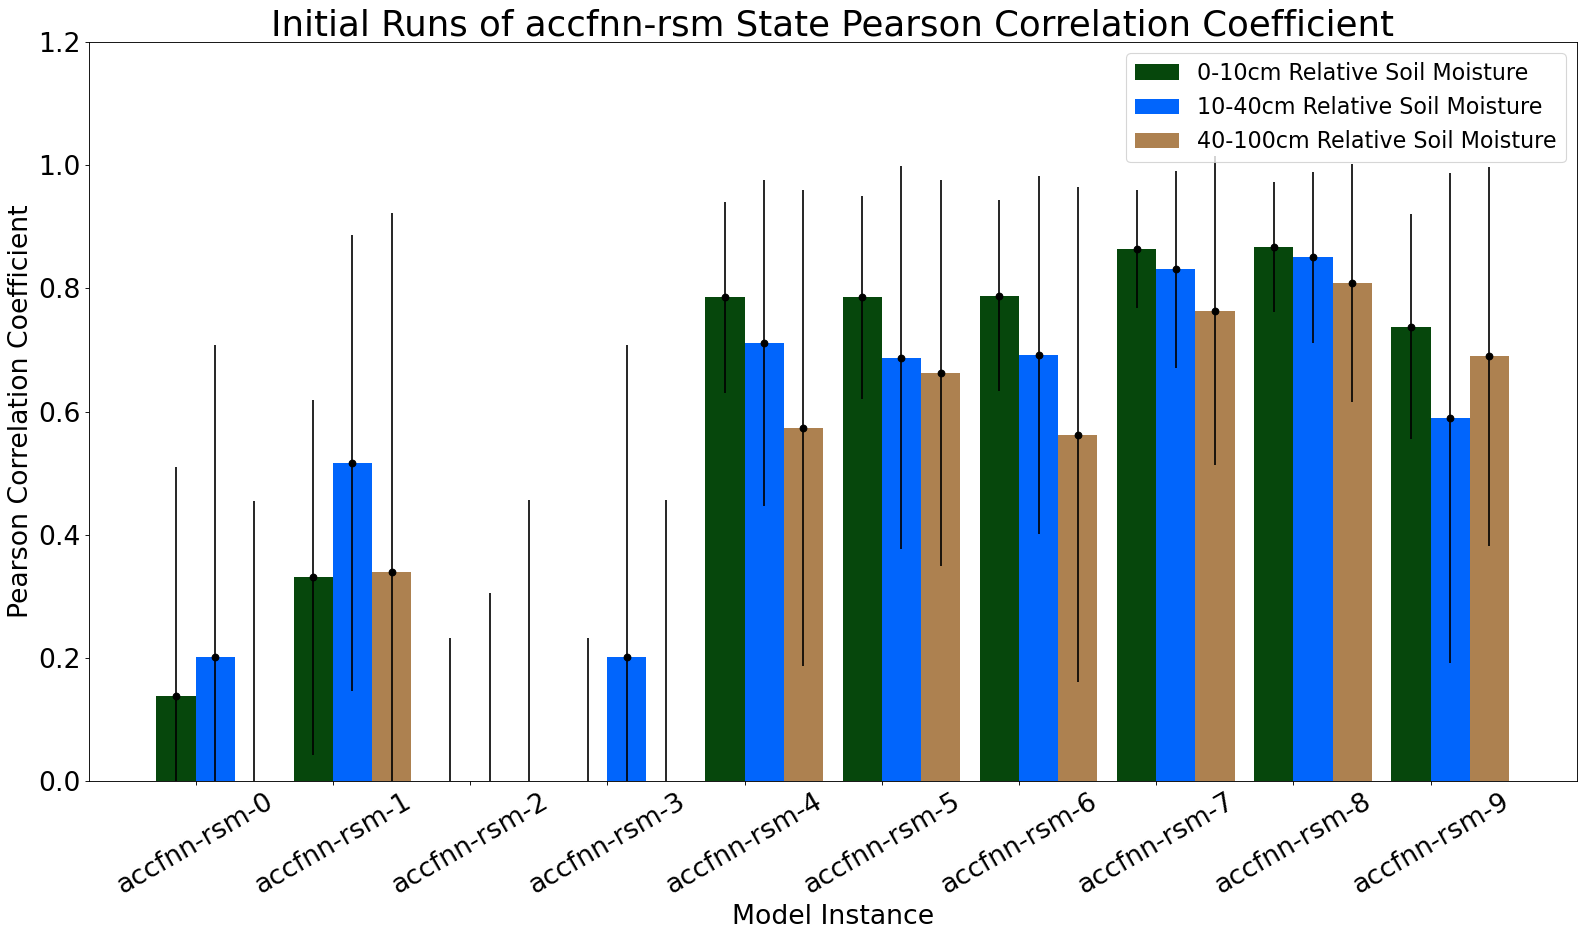
\includegraphics[width=.48\linewidth,draft=false]{figures/efficiency_initial-best/eval_test_efficiency_initial-accfnn-rsm_cc_state.png}

    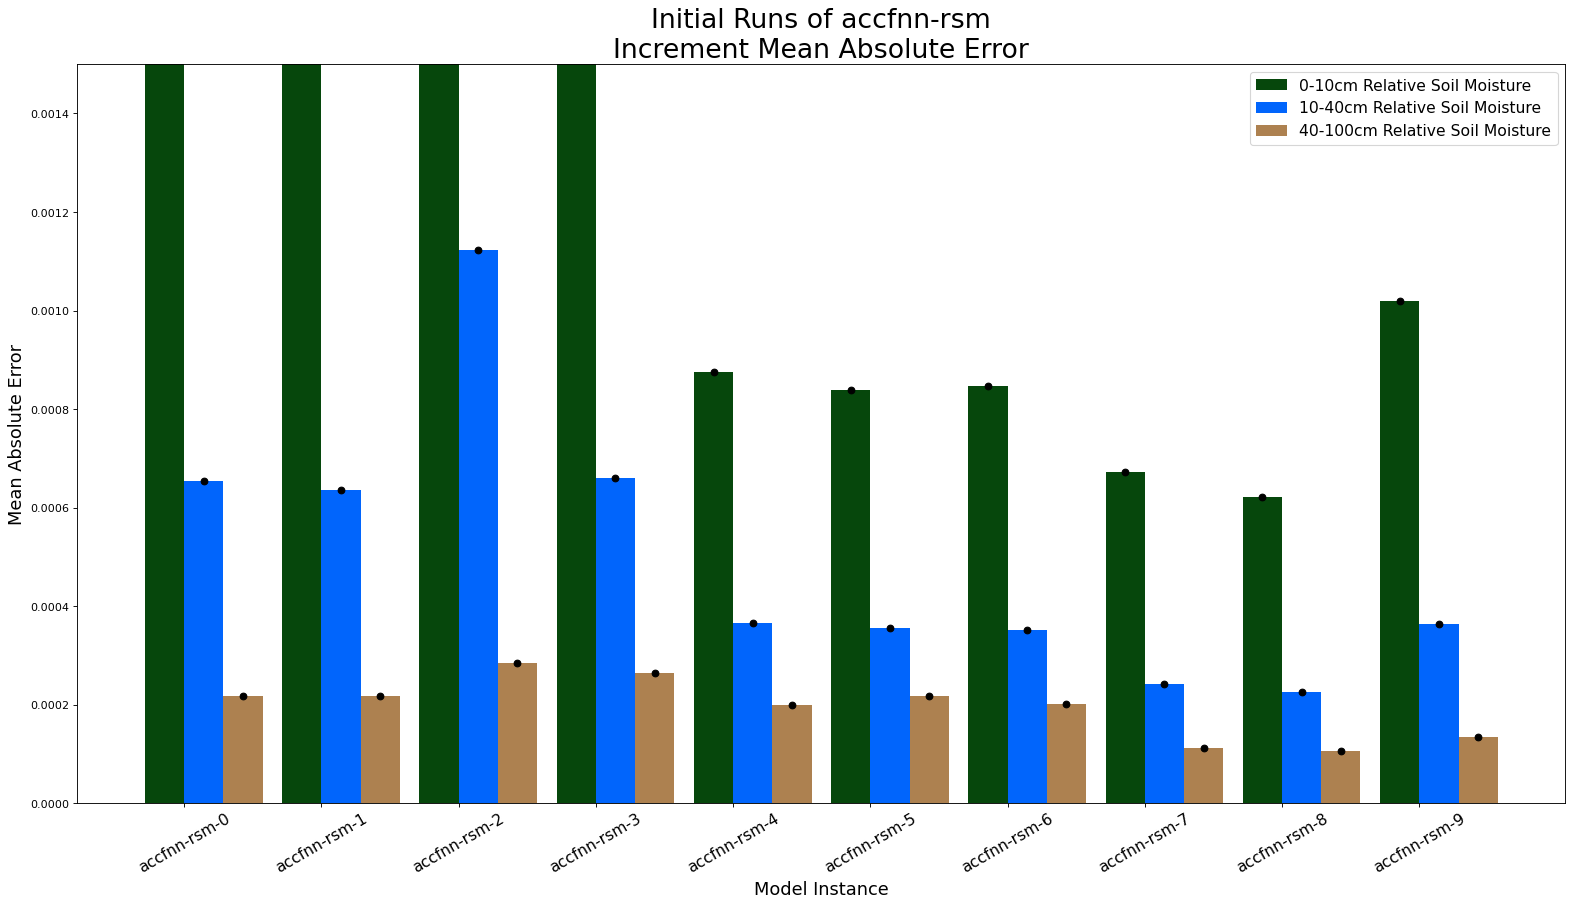
\includegraphics[width=.48\linewidth,draft=false]{figures/efficiency_initial-best/eval_test_efficiency_initial-accfnn-rsm_mae_res.png}
    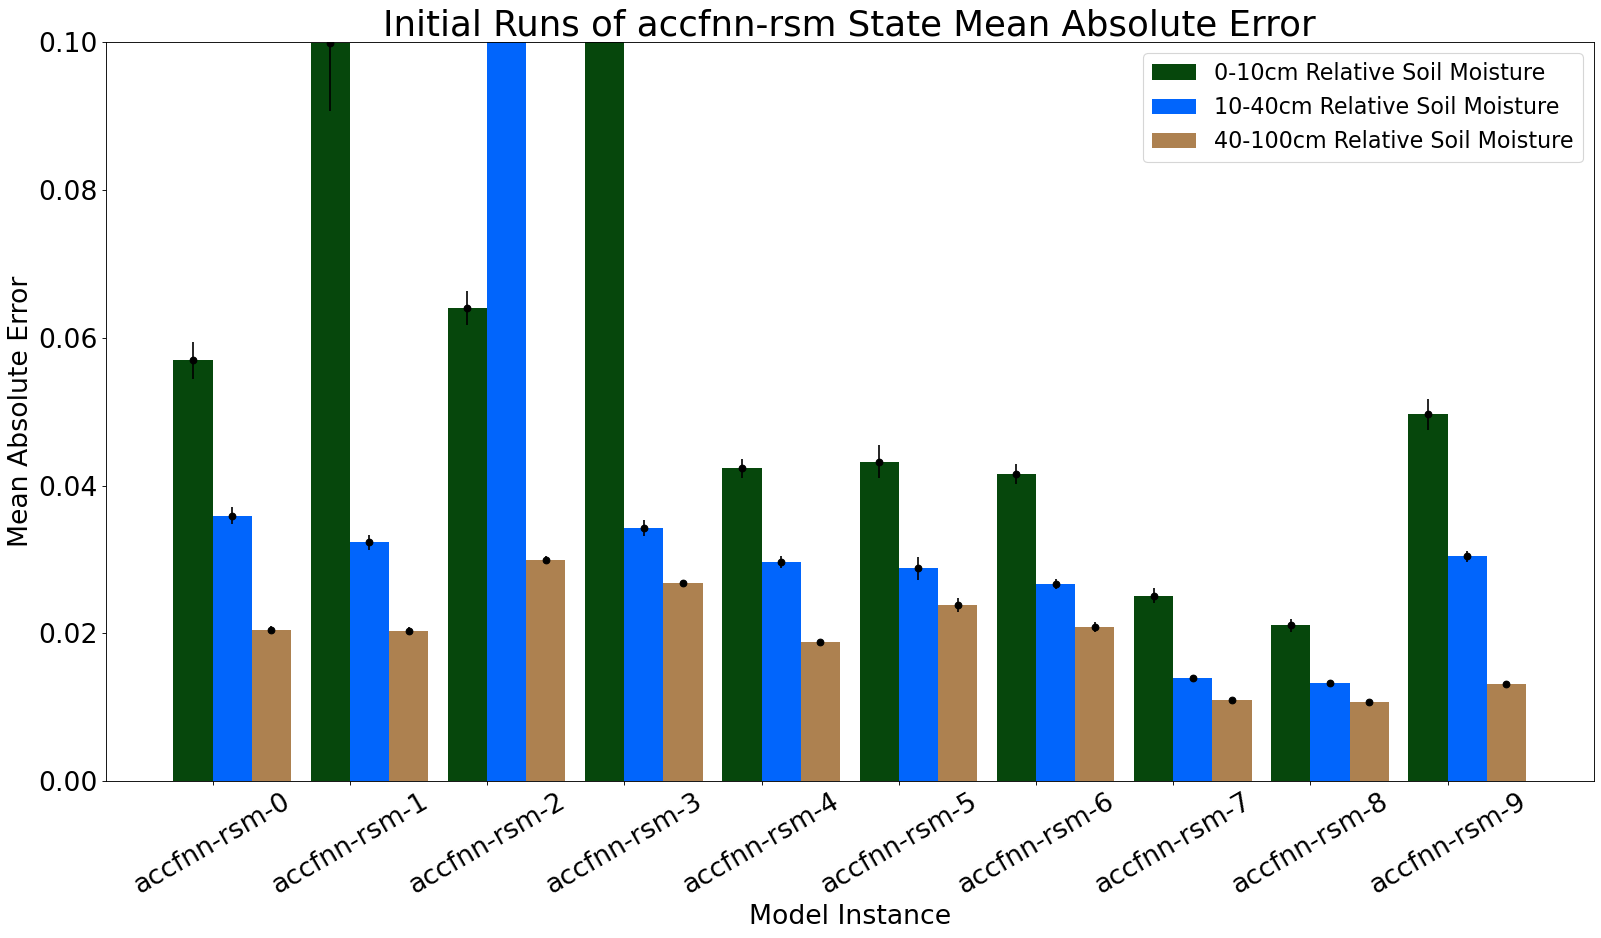
\includegraphics[width=.48\linewidth,draft=false]{figures/efficiency_initial-best/eval_test_efficiency_initial-accfnn-rsm_mae_state.png}

    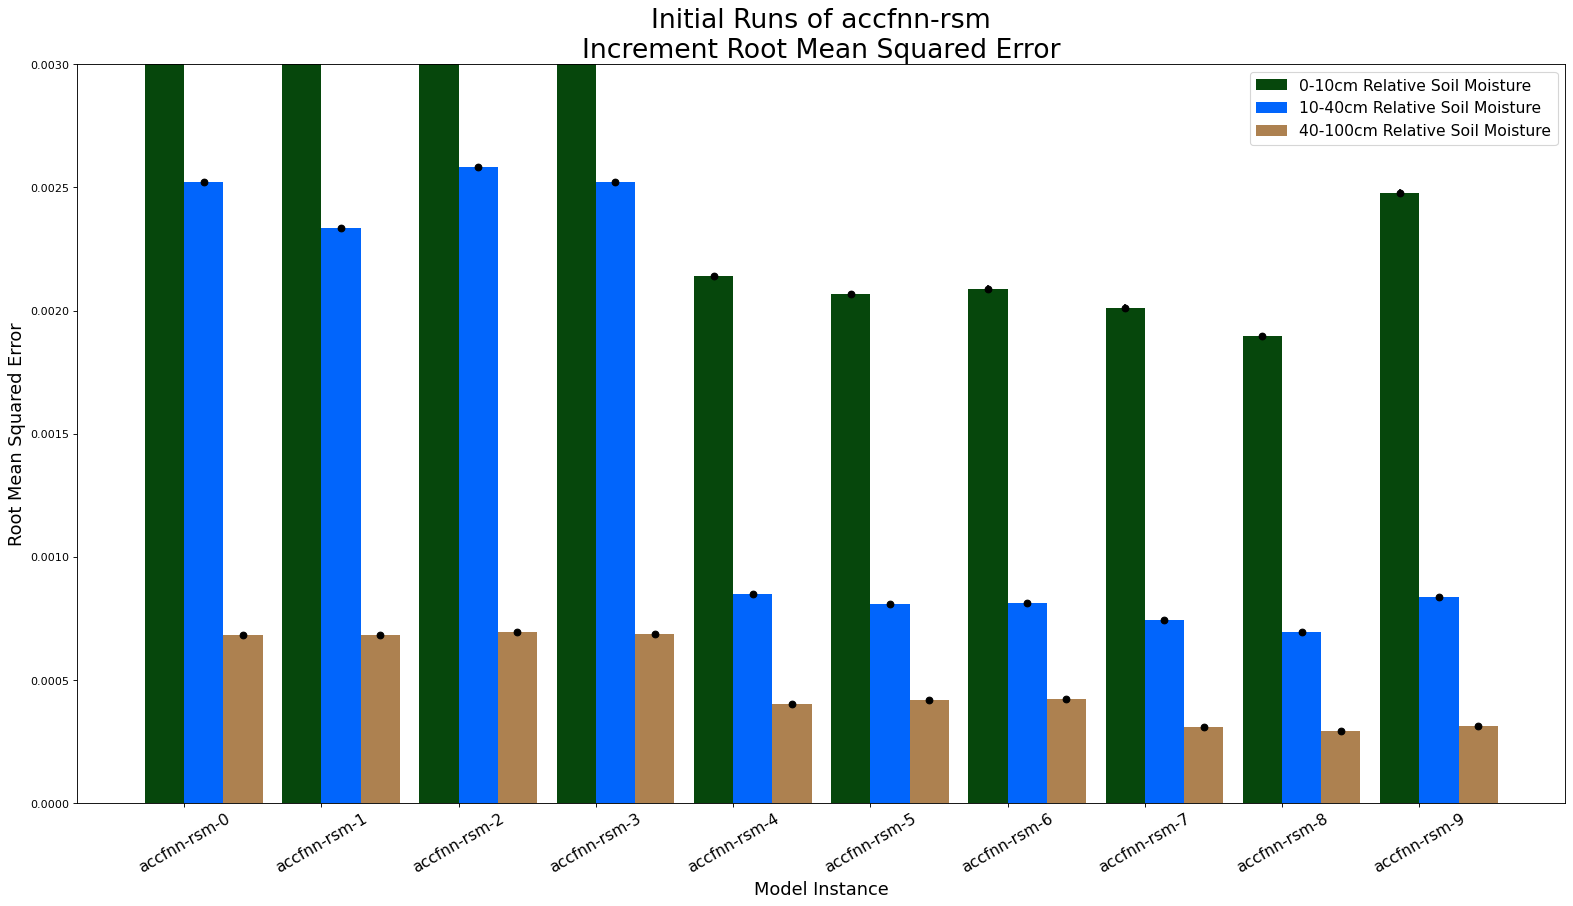
\includegraphics[width=.48\linewidth,draft=false]{figures/efficiency_initial-best/eval_test_efficiency_initial-accfnn-rsm_mse_res.png}
    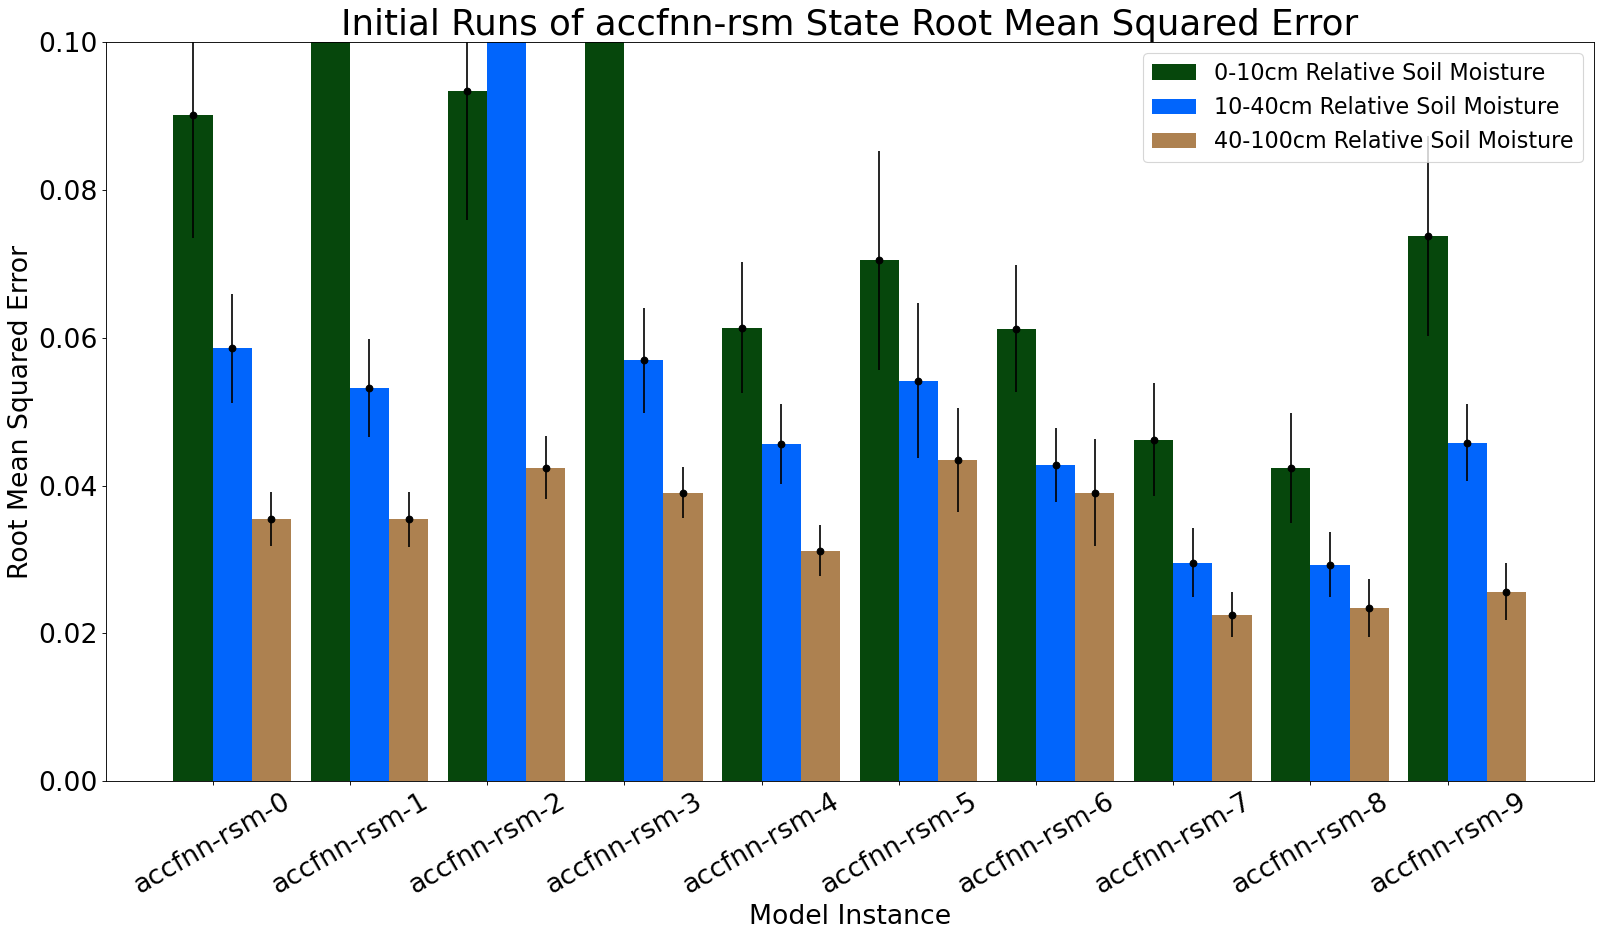
\includegraphics[width=.48\linewidth,draft=false]{figures/efficiency_initial-best/eval_test_efficiency_initial-accfnn-rsm_mse_state.png}

    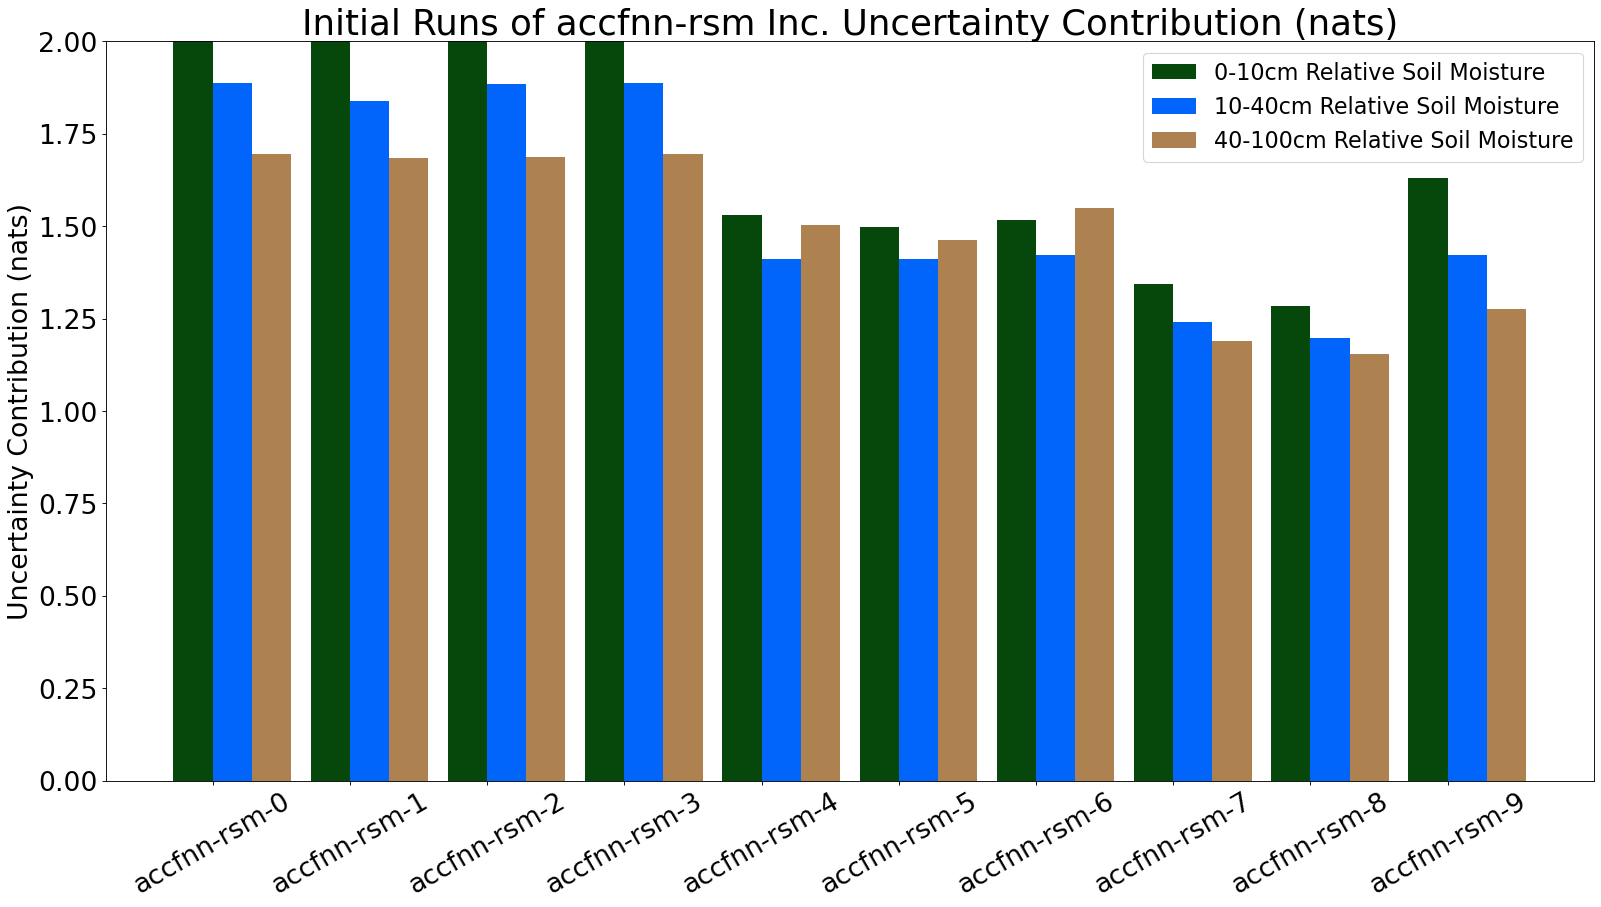
\includegraphics[width=.48\linewidth,draft=false]{figures/efficiency_initial-best/eval_test_efficiency_initial-accfnn-rsm_info-loss_res.png}
    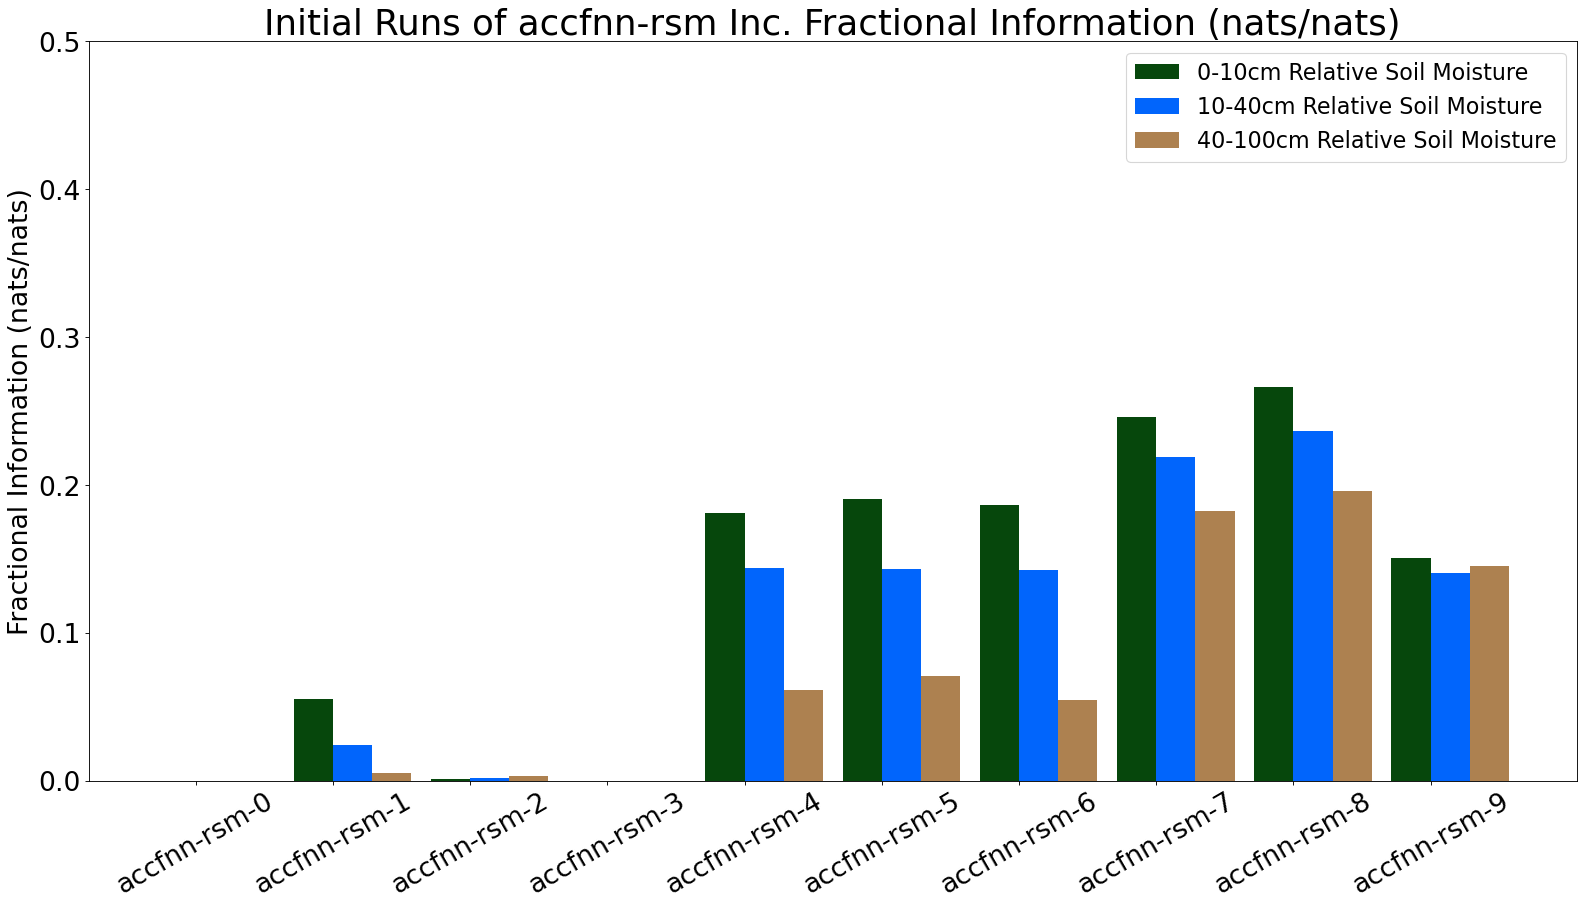
\includegraphics[width=.48\linewidth,draft=false]{figures/efficiency_initial-best/eval_test_efficiency_initial-accfnn-rsm_fi_res.png}

    \caption{Bulk metrics for initial FNN training runs}
    \label{model-init-fnn}
\end{figure}

\begin{table}[H]
\centering
\begin{sideways}
    \begin{tabular}{c|c|c|c|c|c|c }
	\small
Name & Desc & Weights & \thead{State\\MAE} & \thead{State\\CC} & \thead{Info\\Loss} &\thead{Frac.\\Info}\\
\hline
\multirow{3}{6em}{accfnn-rsm-0} & \multirow{3}{16em}{First FNN} & \multirow{3}{4em}{14203} & 0.057 & 0.139 & 2.196 & 0.000 \\ & & & 0.036 & 0.201 & 1.889 & 0.000 \\ & & & 0.020 & -0.215 & 1.694 & 0.000 \\
\hline
\multirow{3}{6em}{accfnn-rsm-1} & \multirow{3}{16em}{Same setup as accrnn-rsm-1 but only a FNN} & \multirow{3}{4em}{14203} & 0.100 & 0.331 & 2.065 & 0.055 \\ & & & 0.032 & 0.517 & 1.840 & 0.024 \\ & & & 0.020 & 0.340 & 1.685 & 0.005 \\
\hline
\multirow{3}{6em}{accfnn-rsm-2} & \multirow{3}{16em}{Much wider and deeper, MSE loss, more dropout} & \multirow{3}{4em}{85947} & 0.064 & -0.139 & 2.193 & 0.001 \\ & & & 0.102 & -0.201 & 1.885 & 0.002 \\ & & & 0.030 & -0.214 & 1.688 & 0.003 \\
\hline
\multirow{3}{6em}{accfnn-rsm-3} & \multirow{3}{16em}{Same as fnn-2 but ignoring constant targets} & \multirow{3}{4em}{85947} & 0.113 & -0.139 & 2.196 & 0.000 \\ & & & 0.034 & 0.201 & 1.889 & 0.000 \\ & & & 0.027 & -0.215 & 1.694 & 0.000 \\
\hline
\multirow{3}{6em}{accfnn-rsm-4} & \multirow{3}{16em}{Same as rsm-2 but no dropout, higher increment magnitude bias} & \multirow{3}{4em}{85947} & 0.042 & 0.786 & 1.530 & 0.181 \\ & & & 0.030 & 0.711 & 1.412 & 0.144 \\ & & & 0.019 & 0.573 & 1.502 & 0.061 \\
\hline
\multirow{3}{6em}{accfnn-rsm-5} & \multirow{3}{16em}{Same as rsm-4 but ignoring constant targets} & \multirow{3}{4em}{85947} & 0.043 & 0.785 & 1.499 & 0.191 \\ & & & 0.029 & 0.688 & 1.411 & 0.143 \\ & & & 0.024 & 0.663 & 1.463 & 0.071 \\
\hline
\multirow{3}{6em}{accfnn-rsm-6} & \multirow{3}{16em}{Same as rsm-4 but narrower and deeper} & \multirow{3}{4em}{30843} & 0.042 & 0.788 & 1.516 & 0.187 \\ & & & 0.027 & 0.692 & 1.423 & 0.142 \\ & & & 0.021 & 0.563 & 1.550 & 0.055 \\
\hline
\multirow{3}{6em}{accfnn-rsm-7} & \multirow{3}{16em}{Same as rsm-6 but mae loss} & \multirow{3}{4em}{30843} & 0.025 & 0.864 & 1.343 & 0.246 \\ & & & 0.014 & 0.831 & 1.242 & 0.219 \\ & & & 0.011 & 0.764 & 1.189 & 0.183 \\
\hline
\multirow{3}{6em}{accfnn-rsm-8} & \multirow{3}{16em}{Same as rsm-7 but ignoring constant targets} & \multirow{3}{4em}{30843} & 0.021 & 0.867 & 1.283 & 0.266 \\ & & & 0.013 & 0.850 & 1.197 & 0.236 \\ & & & 0.011 & 0.809 & 1.154 & 0.196 \\
\hline
\multirow{3}{6em}{accfnn-rsm-9} & \multirow{3}{16em}{fnn 5 but actually using increment norm coefficients} & \multirow{3}{4em}{85947} & 0.050 & 0.738 & 1.632 & 0.151 \\ & & & 0.030 & 0.589 & 1.423 & 0.140 \\ & & & 0.013 & 0.689 & 1.277 & 0.145 \\
    \end{tabular}
\end{sideways}
    \caption{Initial fully-connected neural network properties and bulk statistics.}
    \label{model-init-fnn-table}
\end{table}

All of the bulk statistics in this section are reported in terms of relative soil moisture. The bar charts of correlation coefficient, mean absolute error, and mean squared error separately display the error in hourly increment change and integrated soil state, while the entropy-based metrics (uncertainty contribution and fractional information) are calculated only for the increment change. Tables include metrics for each of the depth levels from top to bottom: 0-10cm, 40-100cm, and 100-200cm.

The validation loss of each of the ANN variants generally stopped decreasing after about 18 hours of training on a CPU, though the training time of individual models unsurprisingly depended most strongly on the size of the model and the learning rate parameters. The models shown here have a number of trainable parameters on the order of 100,000. The best-performing instances of the simplest architecture variant (accfnn-rsm-8) had only about 31,000 parameters and used mean absolute error as the base loss function. The FNN instances struggled to converge any time dropout was used during training, and the predictive skill of best model seemed to improve in the lower two layers in response to a loss function manipulation that ignored prediction cost associated with timesteps where the true magnitude of change in soil moisture state was close to zero. Furthermore, the best FNN did not consider error in state within the loss function (increment loss ratio $\rho = 1$), but was trained with a considerable increment magnitude bias of $\gamma = 60$. The network consisted of 8 fully-connected layers each with 64 nodes.

\begin{figure}[hp!]
    \centering
    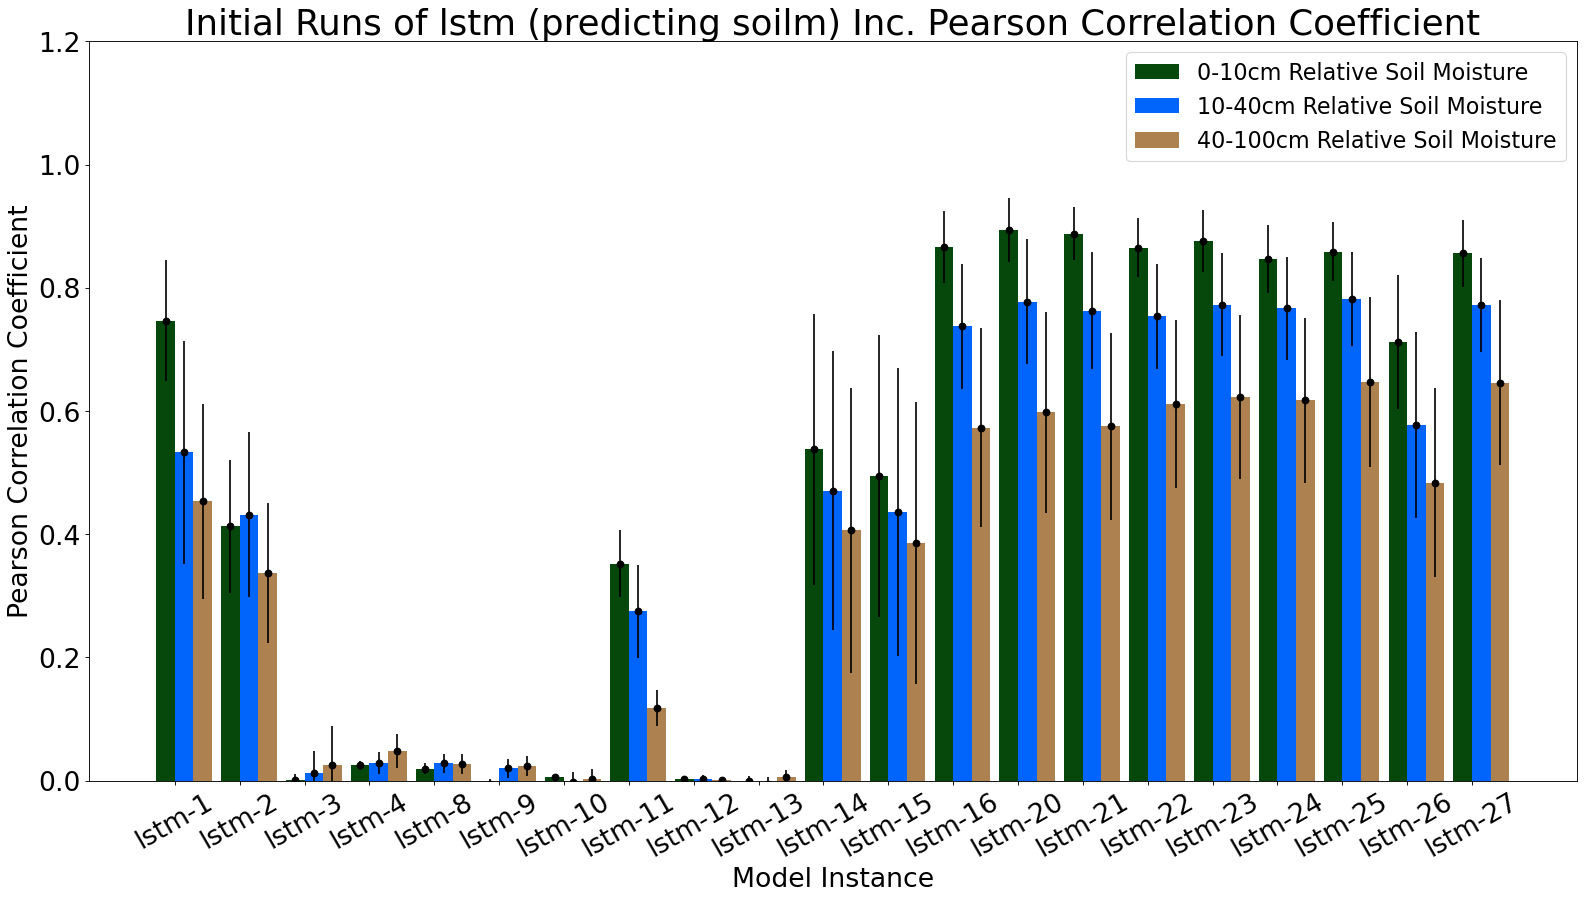
\includegraphics[width=.48\linewidth,draft=false]{figures/efficiency_initial-best/eval_test_efficiency_initial-lstm-soilm_cc_res.png}
    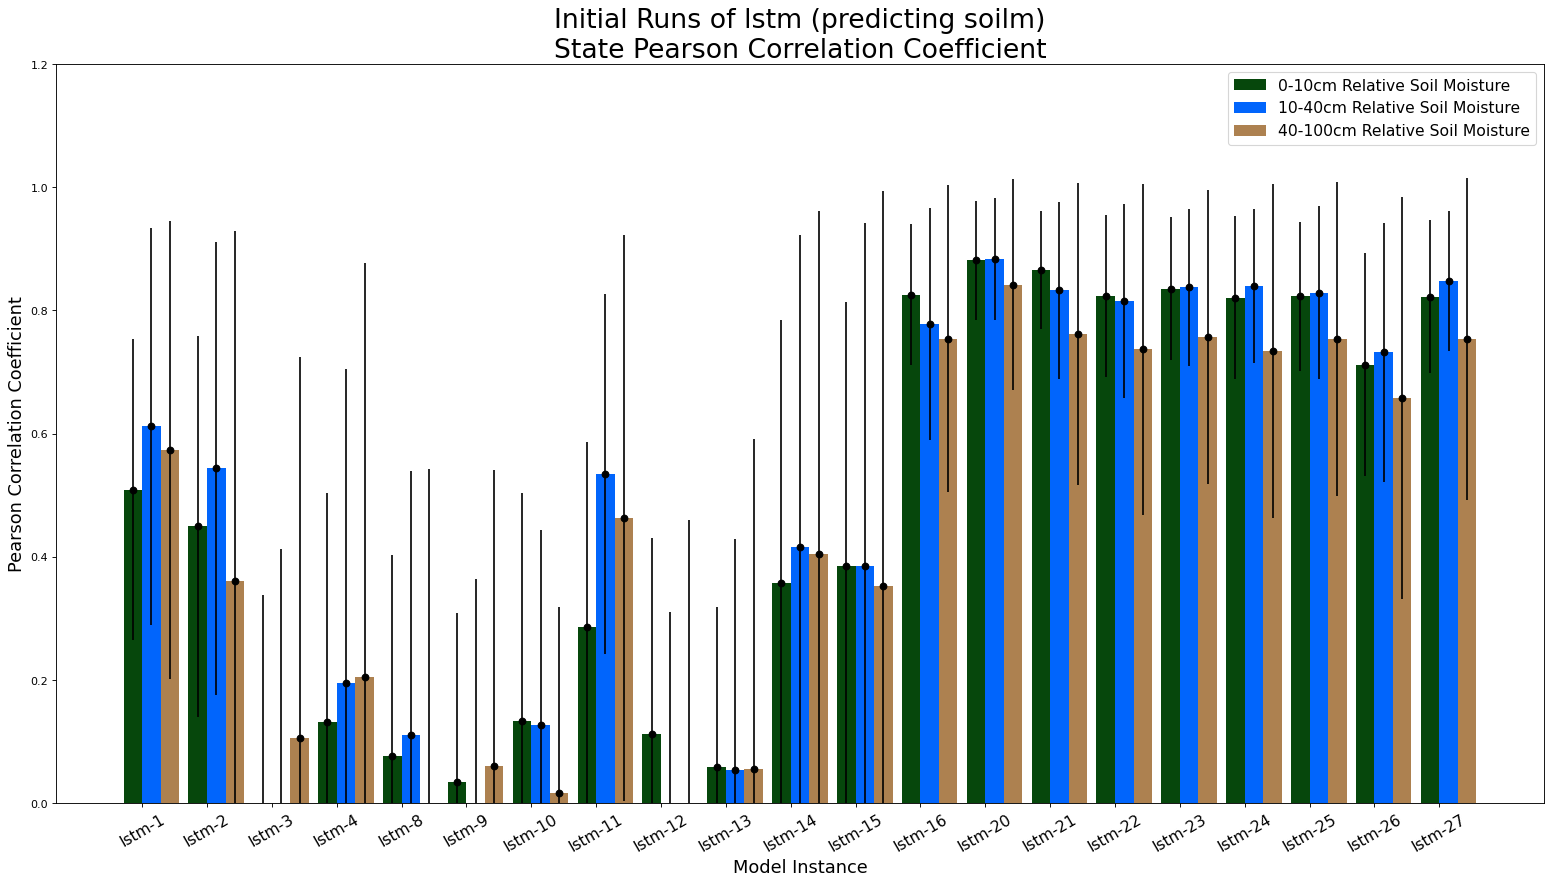
\includegraphics[width=.48\linewidth,draft=false]{figures/efficiency_initial-best/eval_test_efficiency_initial-lstm-soilm_cc_state.png}

    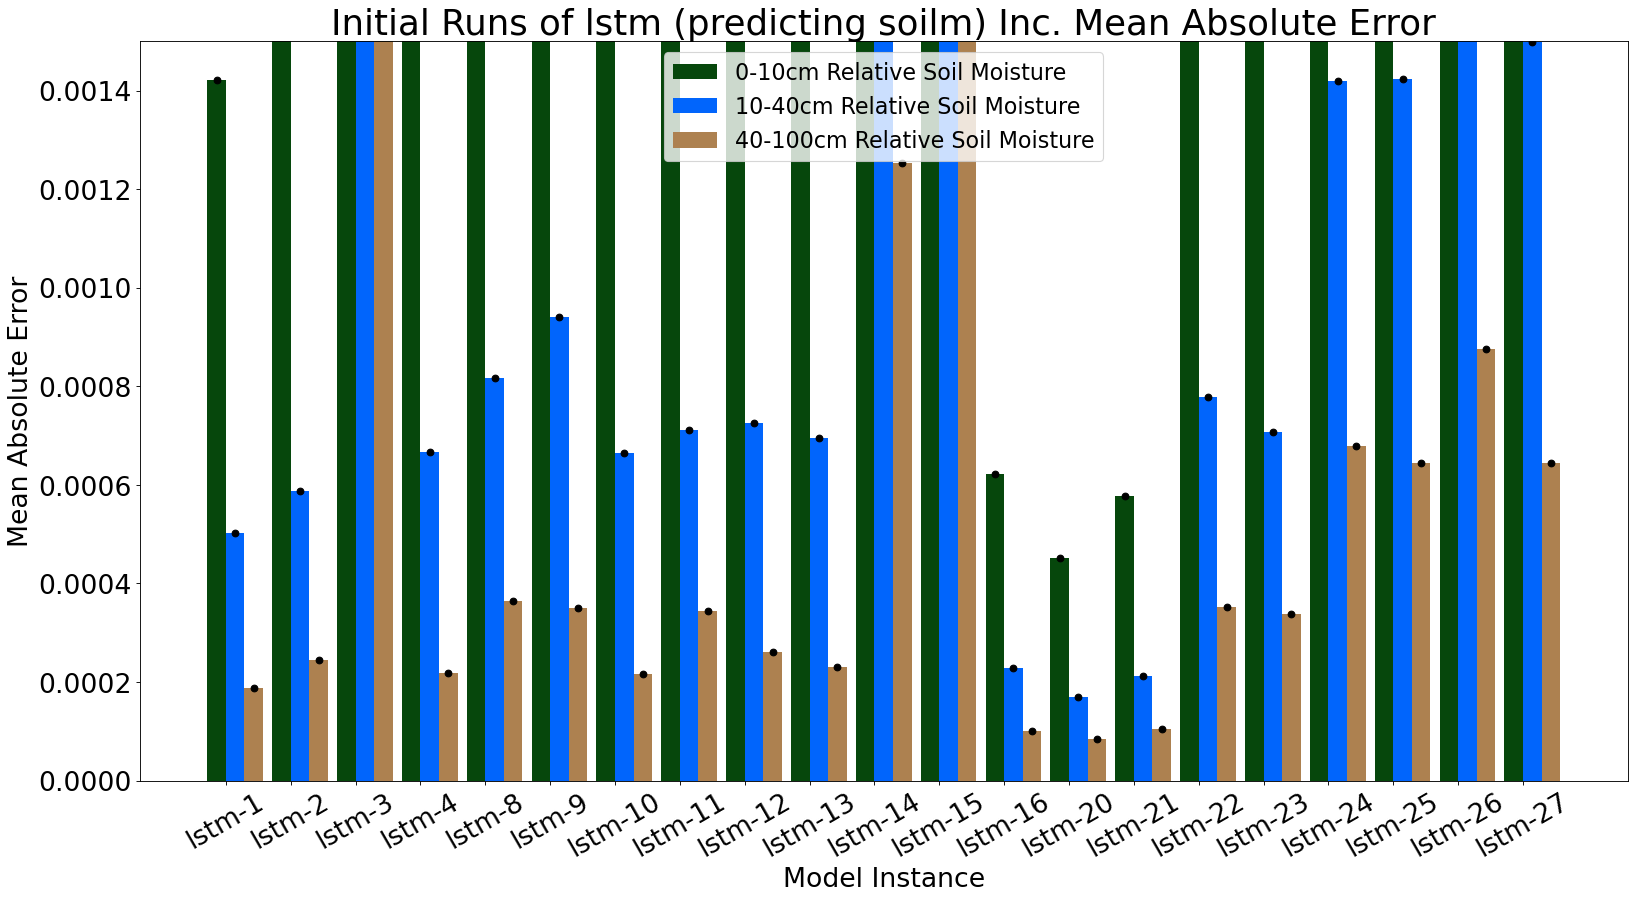
\includegraphics[width=.48\linewidth,draft=false]{figures/efficiency_initial-best/eval_test_efficiency_initial-lstm-soilm_mae_res.png}
    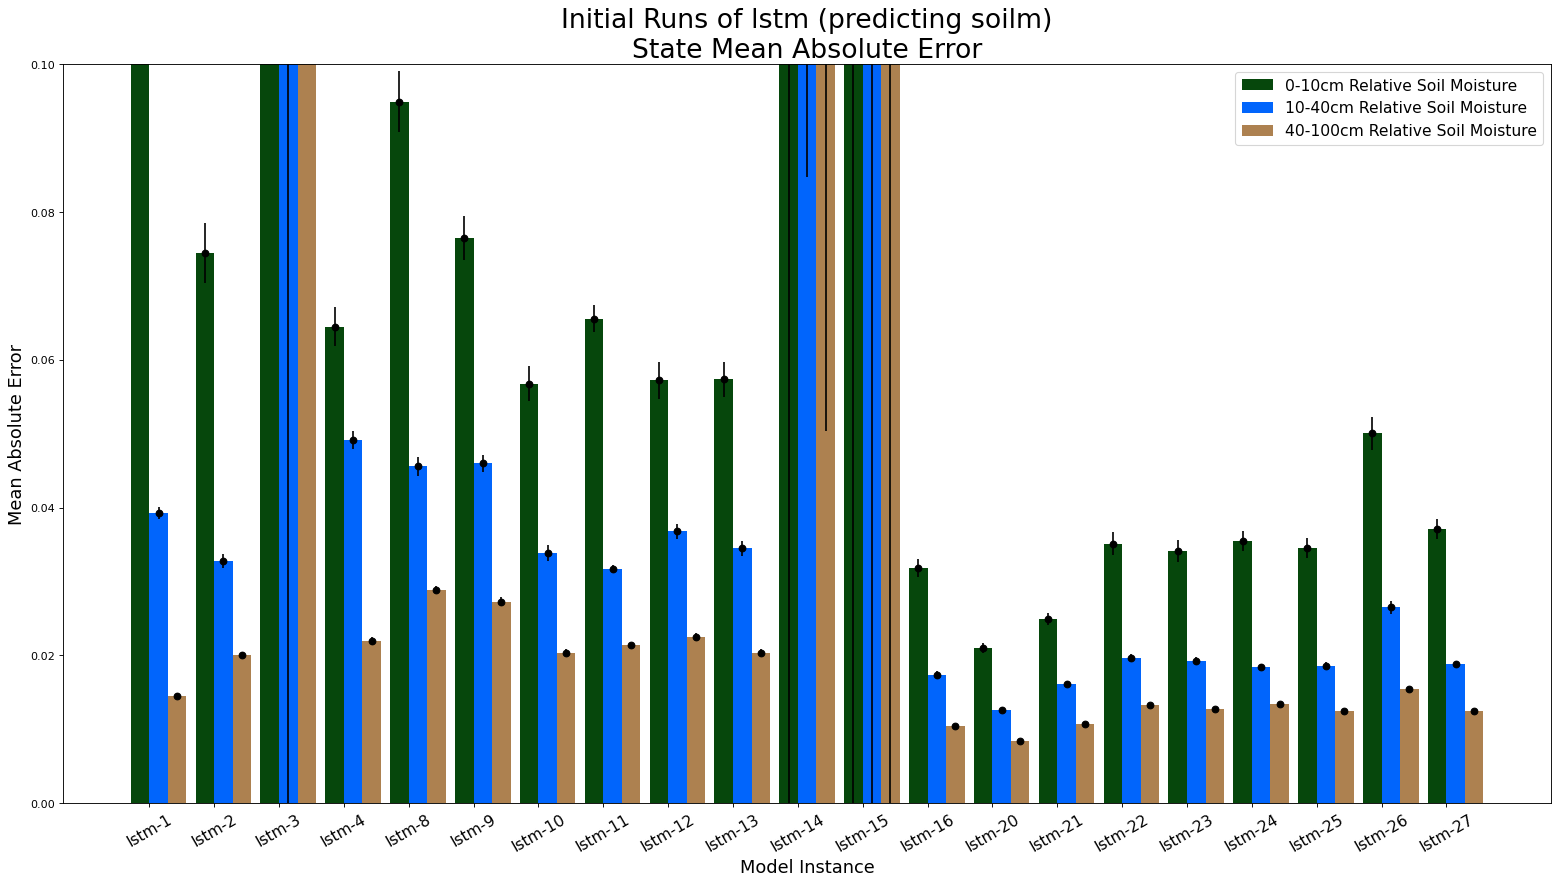
\includegraphics[width=.48\linewidth,draft=false]{figures/efficiency_initial-best/eval_test_efficiency_initial-lstm-soilm_mae_state.png}

    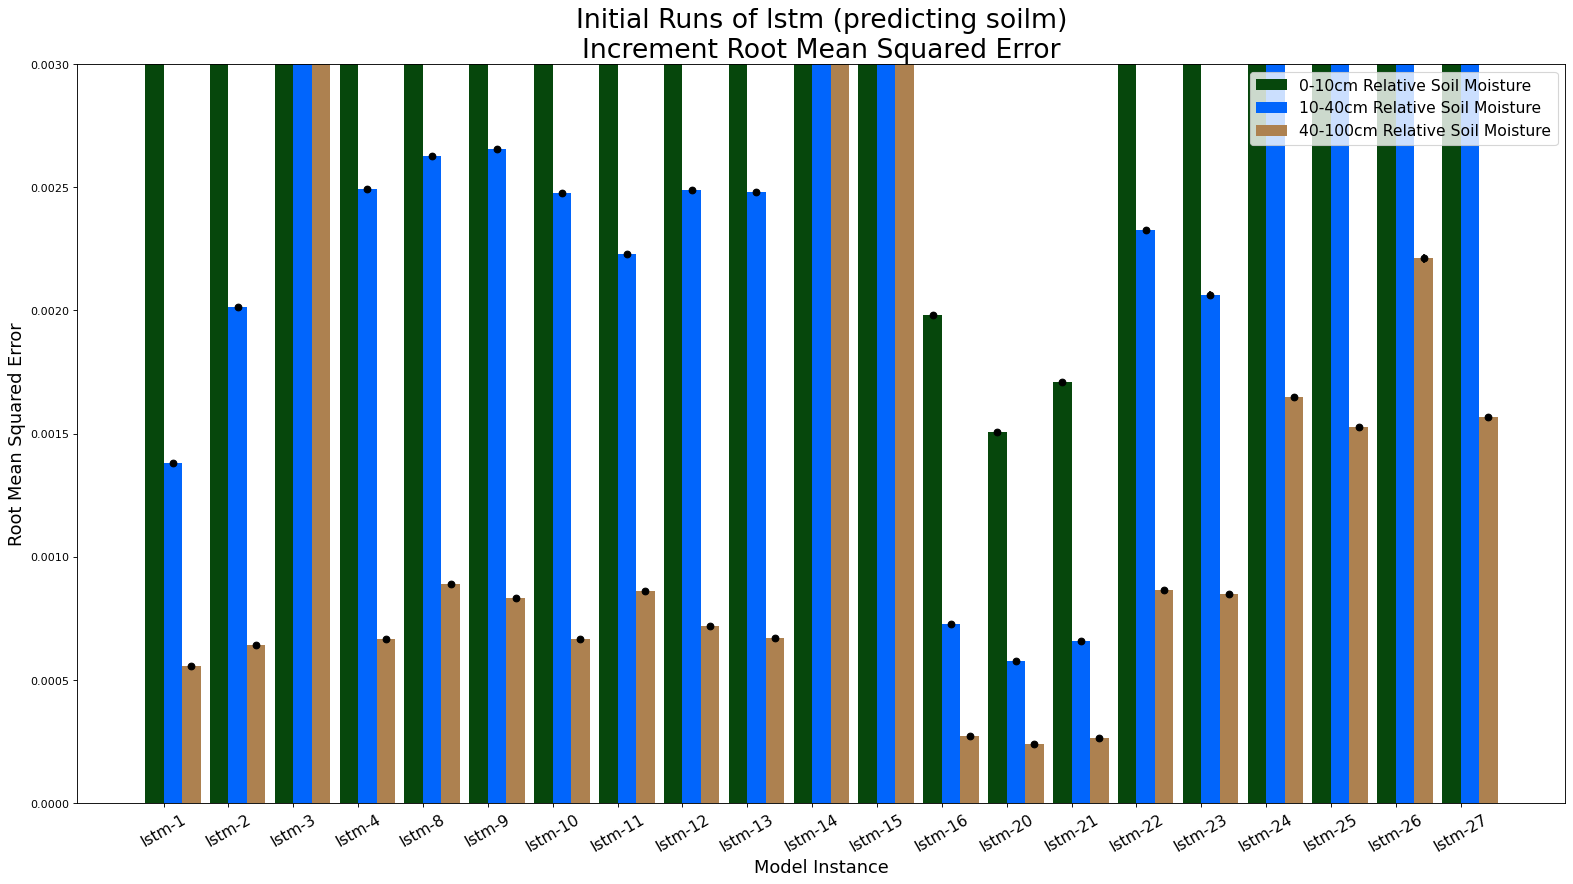
\includegraphics[width=.48\linewidth,draft=false]{figures/efficiency_initial-best/eval_test_efficiency_initial-lstm-soilm_mse_res.png}
    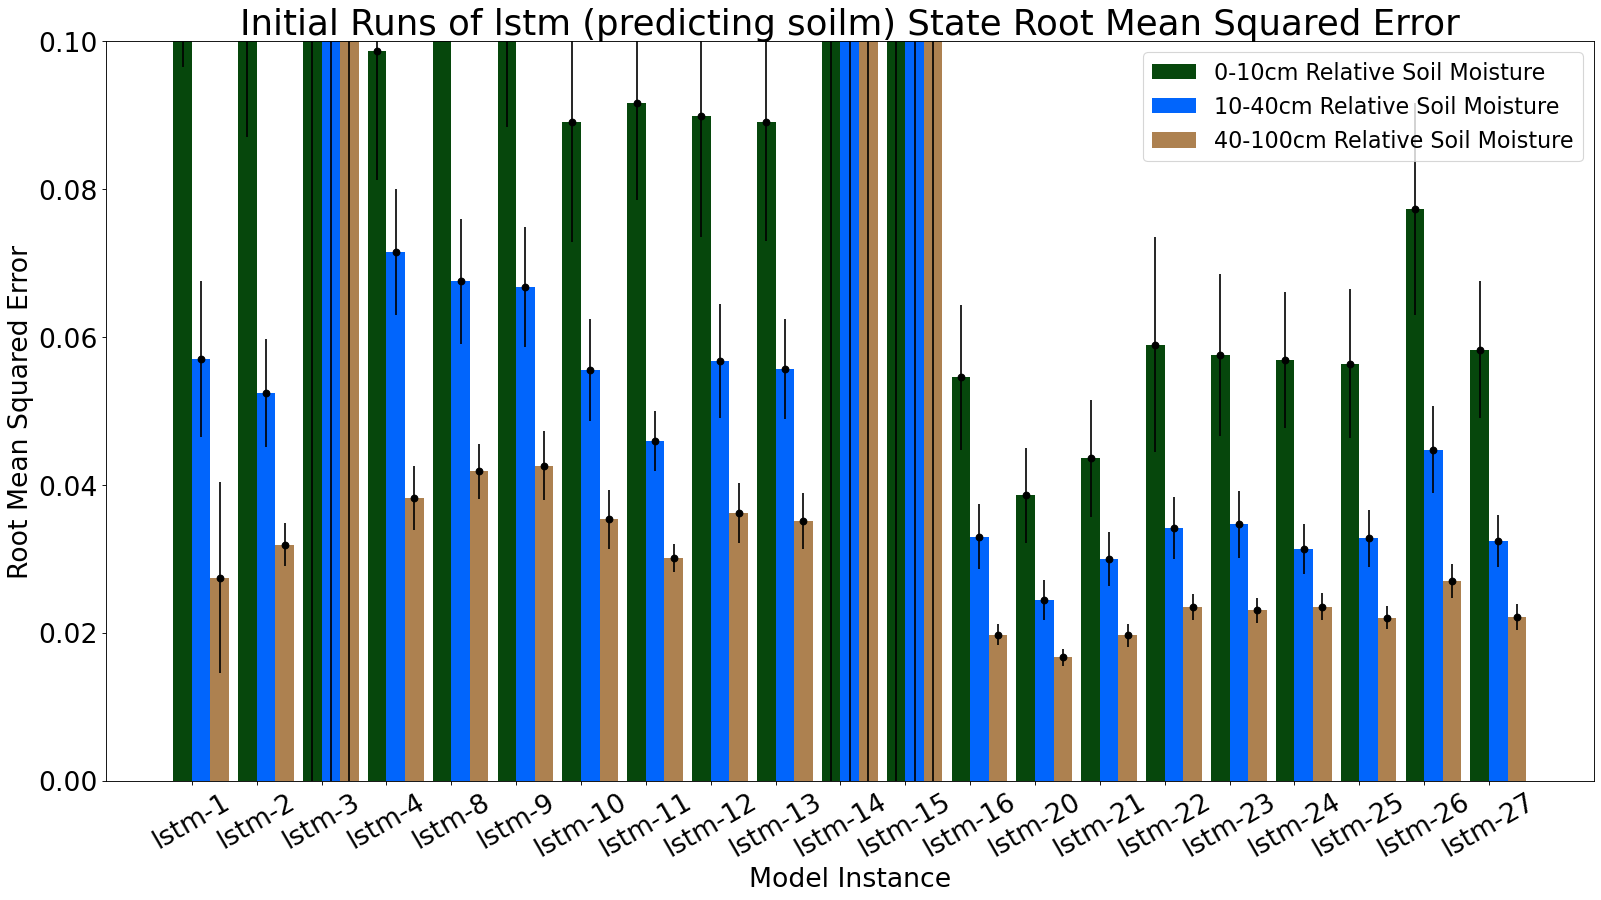
\includegraphics[width=.48\linewidth,draft=false]{figures/efficiency_initial-best/eval_test_efficiency_initial-lstm-soilm_mse_state.png}

    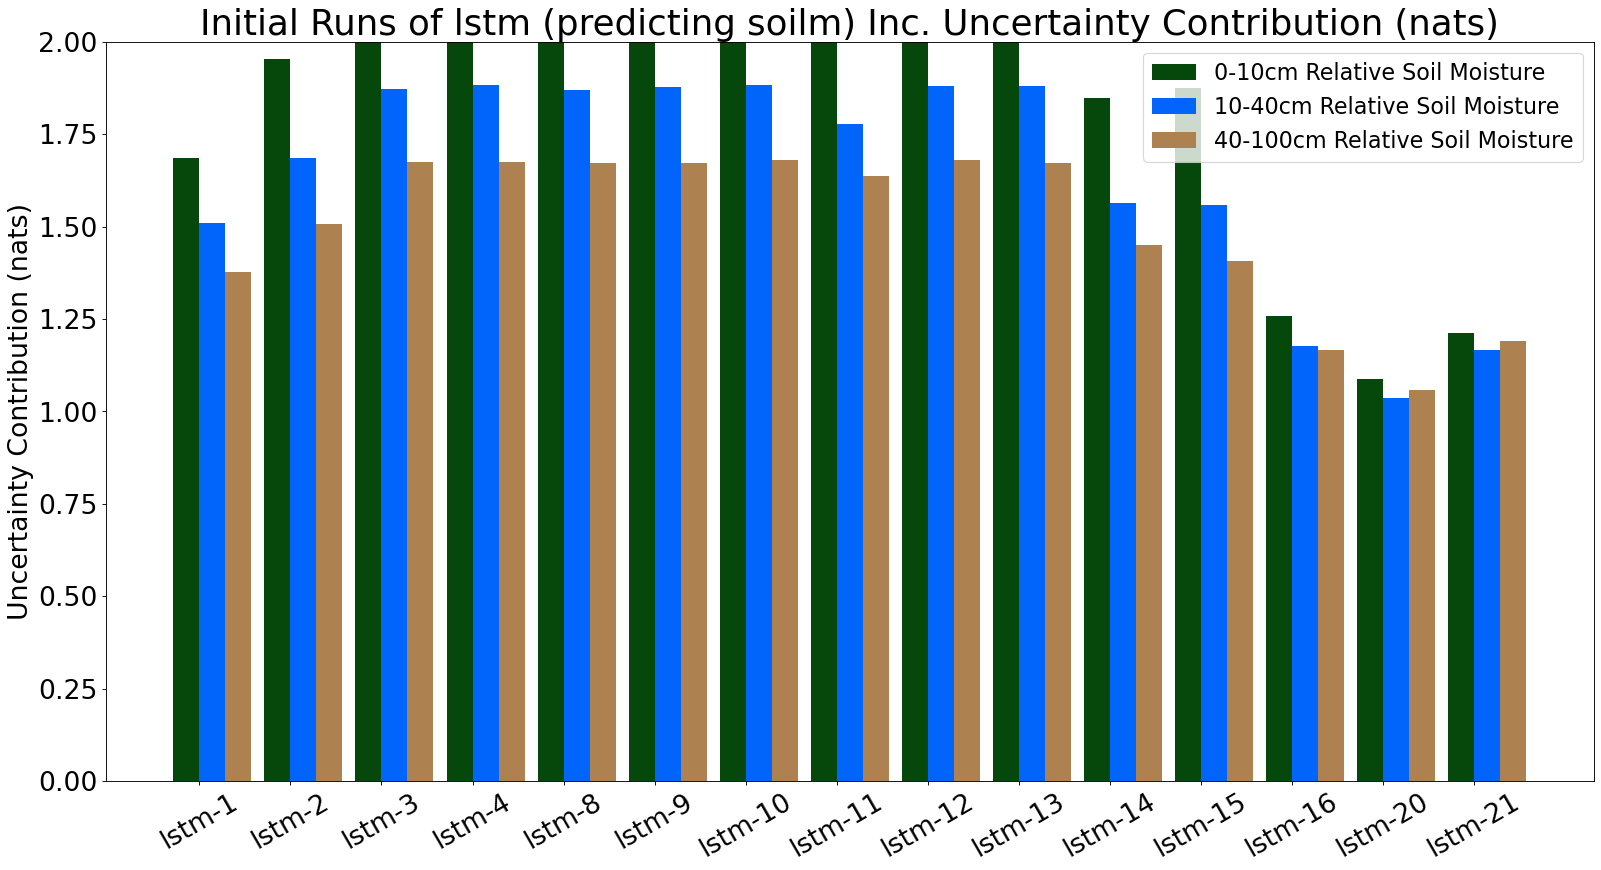
\includegraphics[width=.48\linewidth,draft=false]{figures/efficiency_initial-best/eval_test_efficiency_initial-lstm-soilm_info-loss_res.png}
    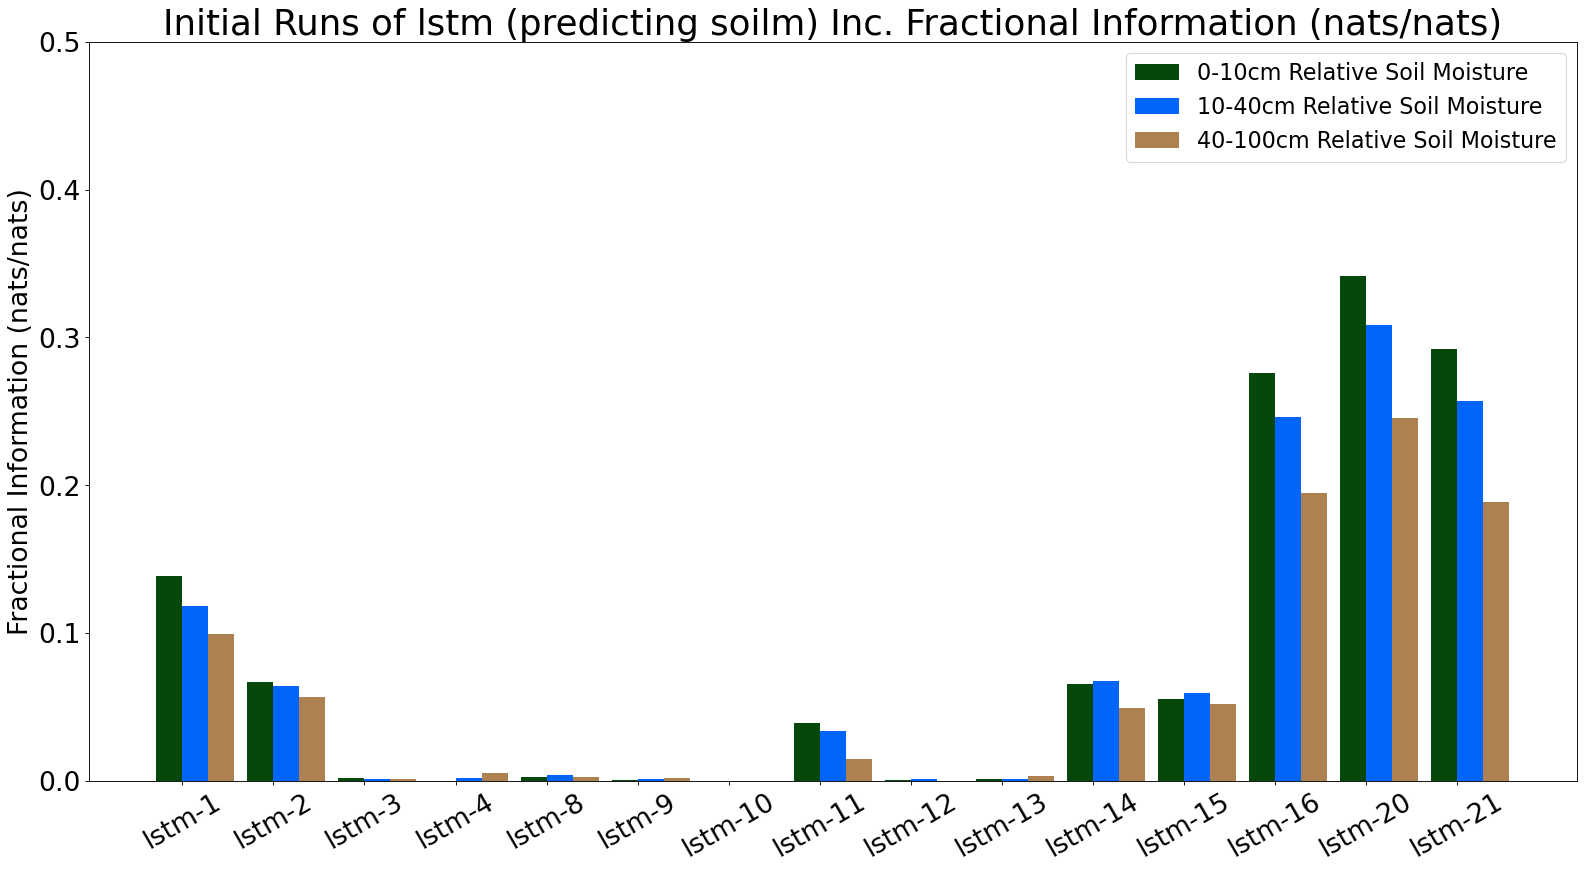
\includegraphics[width=.48\linewidth,draft=false]{figures/efficiency_initial-best/eval_test_efficiency_initial-lstm-soilm_fi_res.png}

    \caption{Bulk metrics for initial LSTM-SOILM training runs}
    \label{model-init-fnn}
\end{figure}

\begin{table}[H]
\begin{sideways}
    \begin{tabular}{c|c|c|c|c|c|c }
    \small
Name & Desc & Weights & \thead{State\\MAE} & \thead{State\\CC} & \thead{Info\\Loss} &\thead{Frac.\\Info}\\
\hline
\multirow{3}{6em}{lstm-1} & \multirow{3}{16em}{4 layers, 64 wide. No batchnorm. } & \multirow{3}{4em}{254397} & 0.107 & 0.509 & 1.686 & 0.138 \\ & & & 0.039 & 0.612 & 1.509 & 0.118 \\ & & & 0.015 & 0.574 & 1.378 & 0.099 \\
\hline
\multirow{3}{6em}{lstm-2} & \multirow{3}{16em}{batchnorm, higher learning rate} & \multirow{3}{4em}{254397} & 0.074 & 0.450 & 1.954 & 0.067 \\ & & & 0.033 & 0.544 & 1.684 & 0.065 \\ & & & 0.020 & 0.360 & 1.507 & 0.057 \\
\hline
\multirow{3}{6em}{lstm-3} & \multirow{3}{16em}{Slower LR ; much 24 wide and 6 layers deep} & \multirow{3}{4em}{64189} & 2.877 & -0.029 & 2.183 & 0.002 \\ & & & 3.153 & -0.084 & 1.873 & 0.002 \\ & & & 0.783 & 0.107 & 1.675 & 0.002 \\
\hline
\multirow{3}{6em}{lstm-4} & \multirow{3}{16em}{4 layers, 96 wide. faster LR, small loss from state magnitude} & \multirow{3}{4em}{629021} & 0.064 & 0.132 & 2.198 & 0.000 \\ & & & 0.049 & 0.196 & 1.882 & 0.002 \\ & & & 0.022 & 0.205 & 1.675 & 0.006 \\
\hline
\multirow{3}{6em}{lstm-8} & \multirow{3}{16em}{4 layers, 64 wide. bigger batch size} & \multirow{3}{4em}{288829} & 0.095 & 0.077 & 2.188 & 0.003 \\ & & & 0.046 & 0.111 & 1.870 & 0.004 \\ & & & 0.029 & -0.034 & 1.671 & 0.003 \\
\hline
\multirow{3}{6em}{lstm-9} & \multirow{3}{16em}{4 layers, 16 wide. bigger batch size} & \multirow{3}{4em}{20029} & 0.076 & 0.035 & 2.195 & 0.000 \\ & & & 0.046 & -0.064 & 1.877 & 0.001 \\ & & & 0.027 & 0.061 & 1.673 & 0.002 \\
\hline
\multirow{3}{6em}{lstm-10} & \multirow{3}{16em}{6 layers, 24 wide; cyclical learning rate ; higher dropout} & \multirow{3}{4em}{65445} & 0.057 & 0.133 & 2.197 & 0.000 \\ & & & 0.034 & 0.127 & 1.882 & 0.000 \\ & & & 0.020 & 0.016 & 1.680 & 0.000 \\
\hline
\multirow{3}{6em}{lstm-11} & \multirow{3}{16em}{2 layers, 256 wide; slower learning rate} & \multirow{3}{4em}{1929597} & 0.066 & 0.286 & 2.058 & 0.039 \\ & & & 0.032 & 0.534 & 1.779 & 0.034 \\ & & & 0.021 & 0.463 & 1.636 & 0.015 \\
\hline
\multirow{3}{6em}{lstm-12} & \multirow{3}{16em}{4 layers, 32 wide; no batchnorm} & \multirow{3}{4em}{74813} & 0.057 & 0.112 & 2.195 & 0.000 \\ & & & 0.037 & -0.193 & 1.880 & 0.001 \\ & & & 0.023 & -0.193 & 1.679 & 0.000 \\
\hline
\multirow{3}{6em}{lstm-13} & \multirow{3}{16em}{same as lstm-12 but increment ratio .8} & \multirow{3}{4em}{74813} & 0.057 & 0.058 & 2.192 & 0.002 \\ & & & 0.034 & 0.055 & 1.879 & 0.001 \\ & & & 0.020 & 0.055 & 1.671 & 0.003 \\
    \end{tabular}
\centering
\end{sideways}
    \caption{Initial LSTM-SOILM properties and bulk statistics (1).}
    \label{model-init-lstm-table-1}
\end{table}

\begin{table}[H]
\begin{sideways}
    \begin{tabular}{c|c|c|c|c|c|c }
    \small
Name & Desc & Weights & \thead{State\\MAE} & \thead{State\\CC} & \thead{Info\\Loss} &\thead{Frac.\\Info}\\
\hline
\multirow{3}{6em}{lstm-14} & \multirow{3}{16em}{Heavy increment error ; decaying log-cyclical learning rate; batch norm} & \multirow{3}{4em}{74813} & 0.726 & 0.357 & 1.847 & 0.065 \\ & & & 0.224 & 0.416 & 1.565 & 0.067 \\ & & & 0.147 & 0.405 & 1.451 & 0.050 \\
\hline
\multirow{3}{6em}{lstm-15} & \multirow{3}{16em}{No dropout, some increment magnitude bias} & \multirow{3}{4em}{74813} & 1.556 & 0.385 & 1.874 & 0.055 \\ & & & 1.481 & 0.385 & 1.558 & 0.060 \\ & & & 0.831 & 0.352 & 1.407 & 0.052 \\
\hline
\multirow{3}{6em}{lstm-16} & \multirow{3}{16em}{Same as lstm-15 but smaller learning rate} & \multirow{3}{4em}{74813} & 0.032 & 0.826 & 1.258 & 0.276 \\ & & & 0.017 & 0.779 & 1.176 & 0.246 \\ & & & 0.010 & 0.754 & 1.166 & 0.195 \\
\hline
\multirow{3}{6em}{lstm-20} & \multirow{3}{16em}{Stronger dependence on state, some increment magnitude bias, dropout} & \multirow{3}{4em}{77117} & 0.021 & 0.882 & 1.088 & 0.342 \\ & & & 0.013 & 0.884 & 1.036 & 0.309 \\ & & & 0.008 & 0.842 & 1.058 & 0.246 \\
\hline
\multirow{3}{6em}{lstm-21} & \multirow{3}{16em}{lstm-20 but more dropout, more increment magnitude bias, some state loss} & \multirow{3}{4em}{77117} & 0.025 & 0.866 & 1.213 & 0.292 \\ & & & 0.016 & 0.833 & 1.166 & 0.257 \\ & & & 0.011 & 0.762 & 1.191 & 0.189 \\
\hline
\multirow{3}{6em}{lstm-22} & \multirow{3}{16em}{4 layers, 32 wide, faster learning rate} & \multirow{3}{4em}{80221} & 0.035 & 0.823 &  &  \\ & & & 0.020 & 0.816 &  &  \\ & & & 0.013 & 0.737 &  &  \\
\hline
\multirow{3}{6em}{lstm-23} & \multirow{3}{16em}{much smaller encoder, heavier on increment, but less magnitude bias} & \multirow{3}{4em}{43597} & 0.034 & 0.835 &  &  \\ & & & 0.019 & 0.838 &  &  \\ & & & 0.013 & 0.756 &  &  \\
\hline
\multirow{3}{6em}{lstm-24} & \multirow{3}{16em}{64 nodes wide, 5 layers deep; weaker dependence on increment, strong increment magnitude bias} & \multirow{3}{4em}{173165} & 0.035 & 0.821 &  &  \\ & & & 0.018 & 0.840 &  &  \\ & & & 0.013 & 0.735 &  &  \\
\hline
\multirow{3}{6em}{lstm-25} & \multirow{3}{16em}{Same as lstm-24, but 128 nodes wide} & \multirow{3}{4em}{364029} & 0.035 & 0.823 &  &  \\ & & & 0.019 & 0.829 &  &  \\ & & & 0.012 & 0.754 &  &  \\
\hline
\multirow{3}{6em}{lstm-26} & \multirow{3}{16em}{Same as lstm-25, 6 layers deep} & \multirow{3}{4em}{762413} & 0.050 & 0.712 &  &  \\ & & & 0.026 & 0.732 &  &  \\ & & & 0.015 & 0.658 &  &  \\
\hline
\multirow{3}{6em}{lstm-27} & \multirow{3}{16em}{Same as lstm-24, more increment error} & \multirow{3}{4em}{173165} & 0.037 & 0.822 &  &  \\ & & & 0.019 & 0.848 &  &  \\ & & & 0.012 & 0.754 &  &  \\
    \end{tabular}
\centering
\end{sideways}
    \caption{Initial LSTM-SOILM properties and bulk statistics (2).}
    \label{model-init-lstm-table-2}
\end{table}

Next, we present a variety of LSTM instances that predict the increment change in volumetric soil moisture ($\frac{kg}{m^2}$), which we will refer to as the LSTM-SOILM group. The results reported here have been converted to relative soil moisture after-the-fact for consistency with the other architectures. In practice, these were the first generations of models we tested; those which appear in Table \ref{model-init-lstm-table-1} were trained using a consistent learning rate and converged rapidly to fairly poor results. Even relatively large models with a variety of hyperparameter configurations didn't achieve a correlation coefficient higher than .65 for any of the layers. Introducing the log-cyclical learning rate schedule prolonged training and, combined with the loss function modifications, resulted in considerably better-performing LSTMs. Given its apparent success, we continued to use the log-cyclical learning rate strategy for the remainder of the models, changing only the rate of decay and the initial minima and maxima of the oscillations. The best LSTM-SOILM models we trained had 77,117 trainable weights, a magnitude bias parameter of $\gamma = 10$, increment loss ratio $\rho = .999$, and did not use increment normalization within the loss function. Unlike the FNN architectures, the best LSTM-SOILM variants tended to include a small weight dropout of 5\% during training, however without further analysis it is difficult to draw conclusions on the actual impact of any of these changes in isolation.

\begin{figure}[hp!]
    \centering
    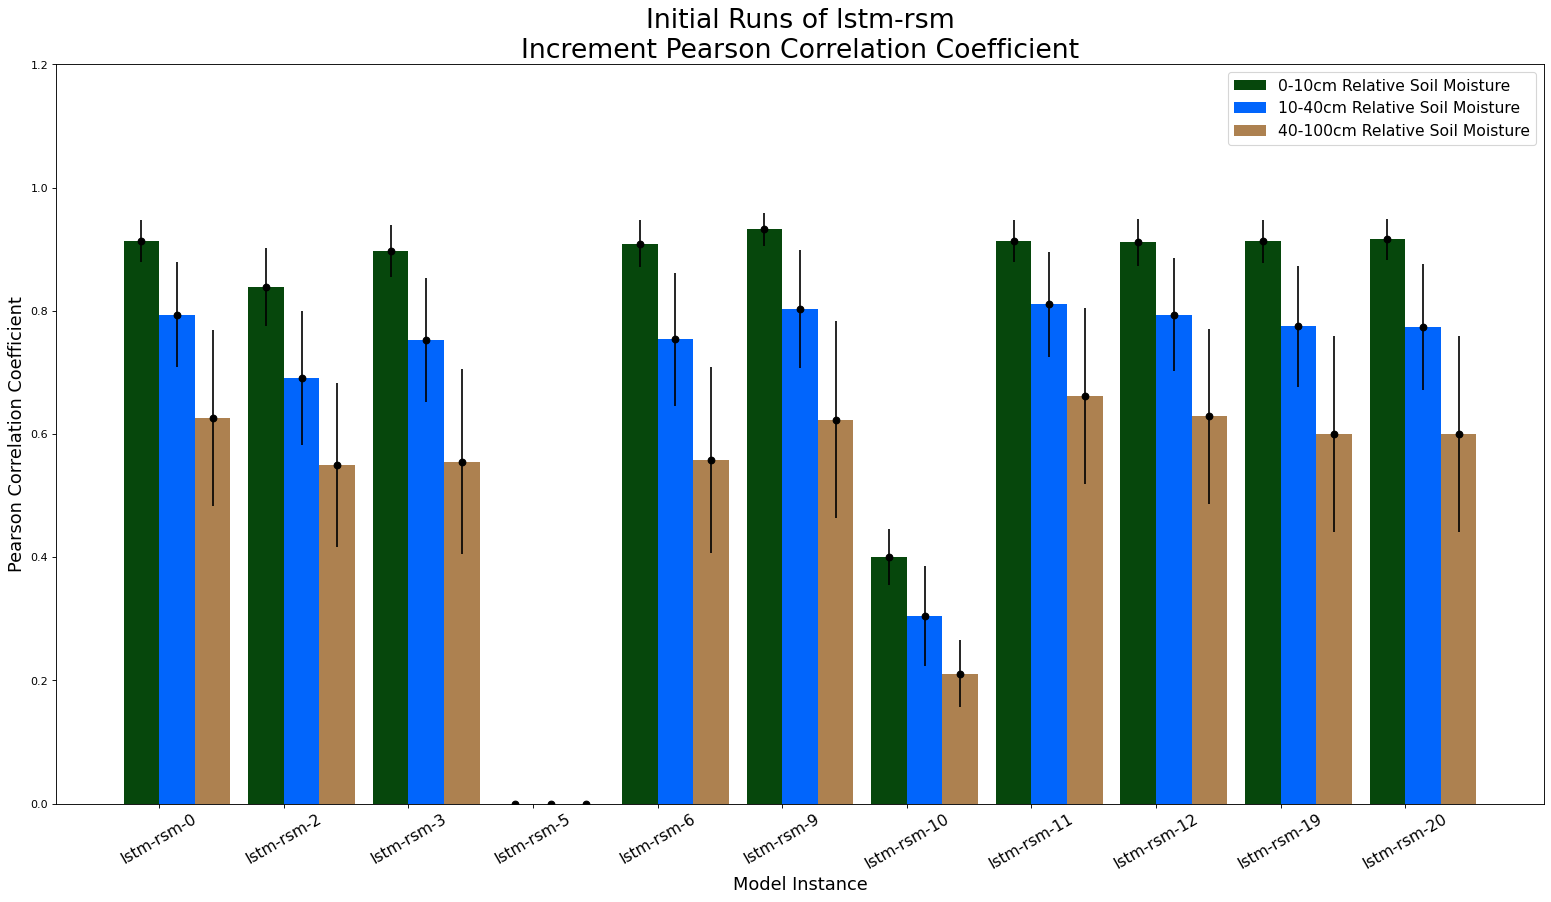
\includegraphics[width=.48\linewidth,draft=false]{figures/efficiency_initial-best/eval_test_efficiency_initial-lstm-rsm_cc_res.png}
    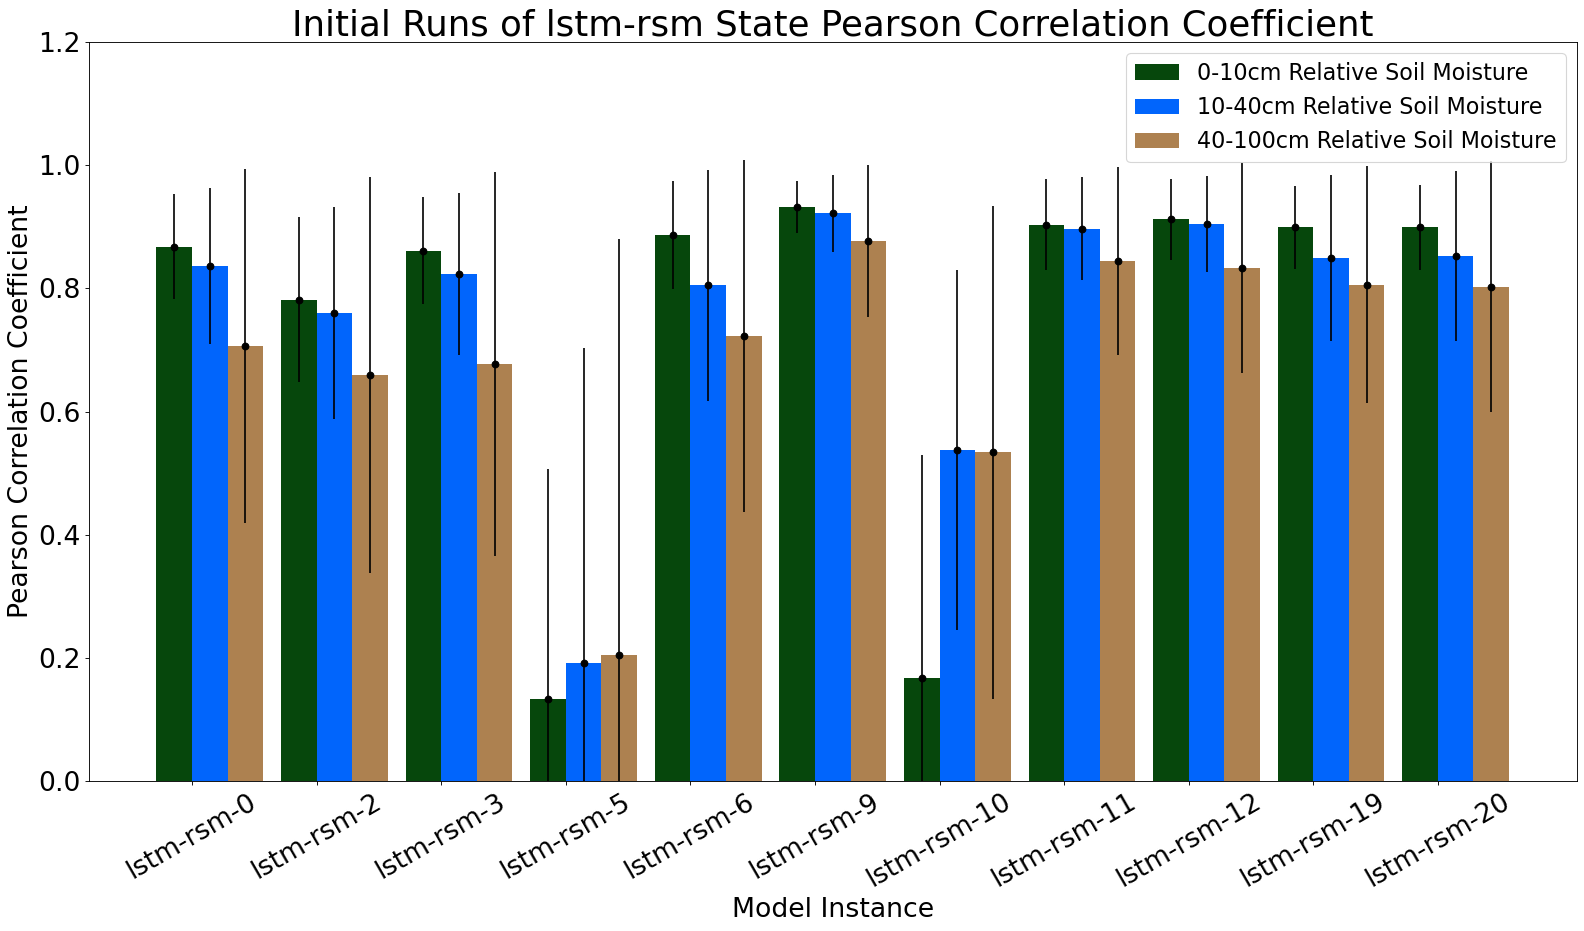
\includegraphics[width=.48\linewidth,draft=false]{figures/efficiency_initial-best/eval_test_efficiency_initial-lstm-rsm_cc_state.png}

    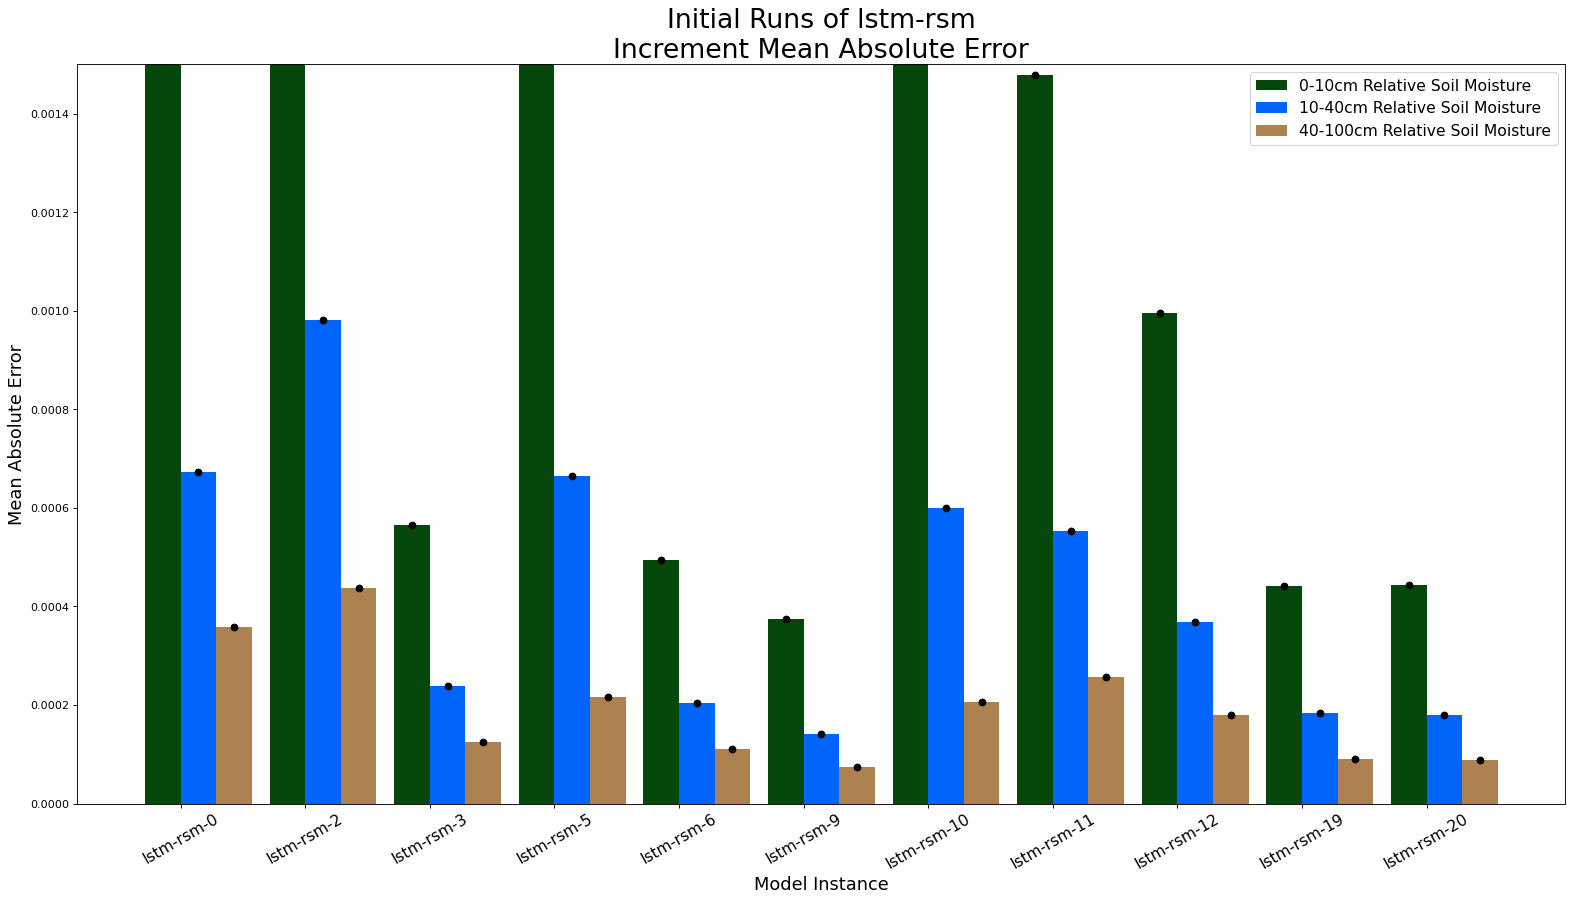
\includegraphics[width=.48\linewidth,draft=false]{figures/efficiency_initial-best/eval_test_efficiency_initial-lstm-rsm_mae_res.png}
    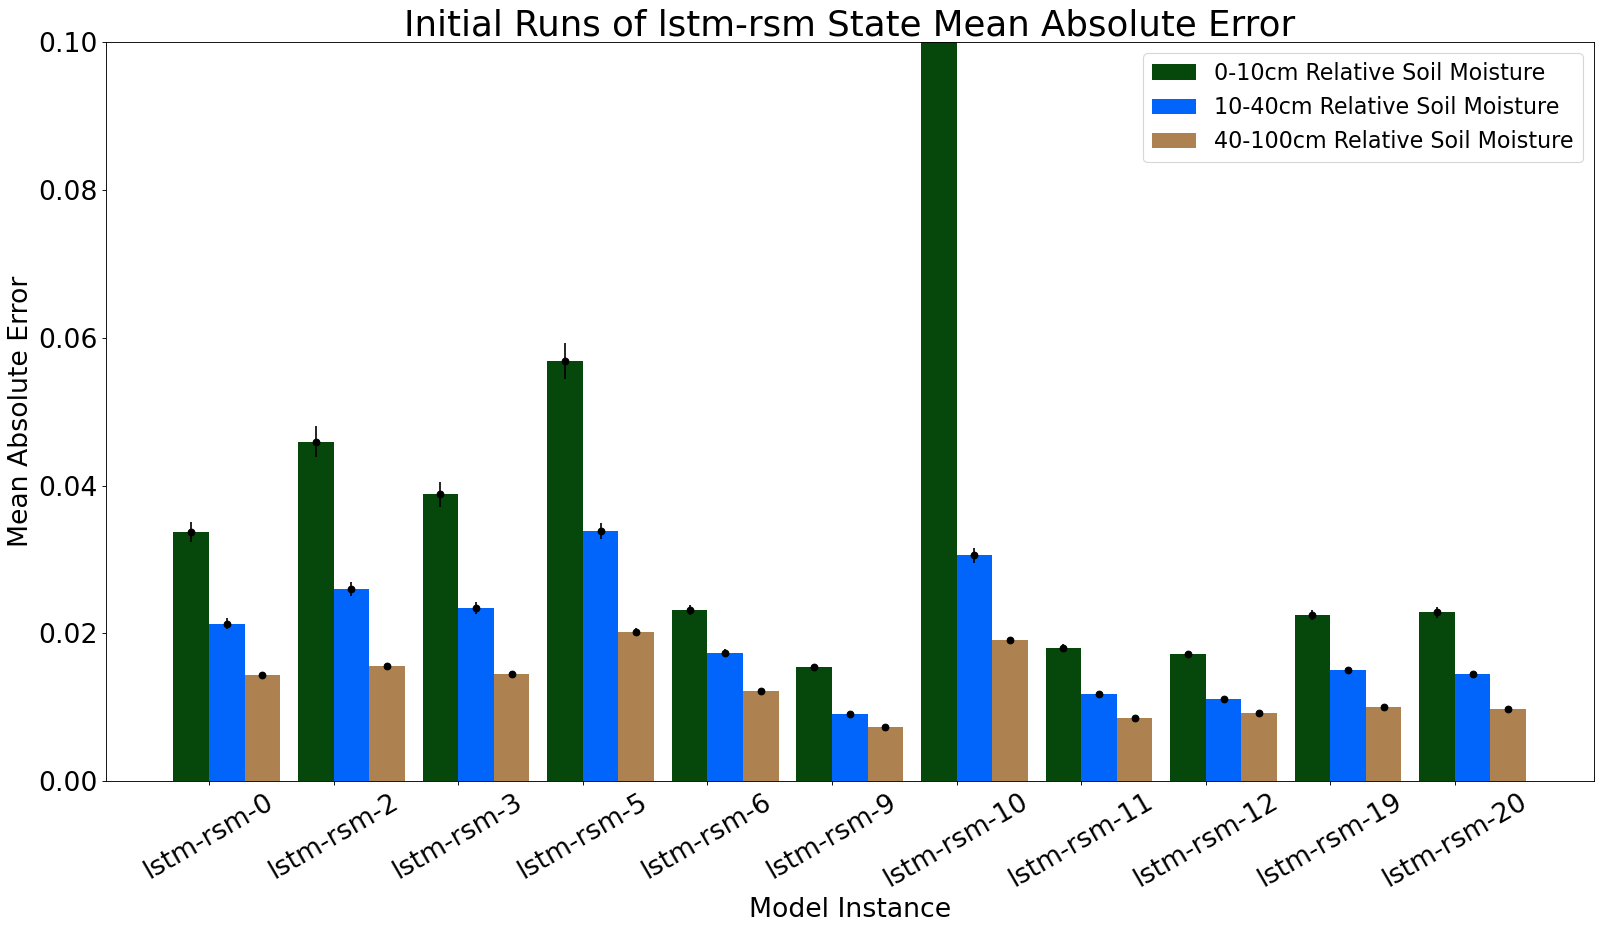
\includegraphics[width=.48\linewidth,draft=false]{figures/efficiency_initial-best/eval_test_efficiency_initial-lstm-rsm_mae_state.png}

    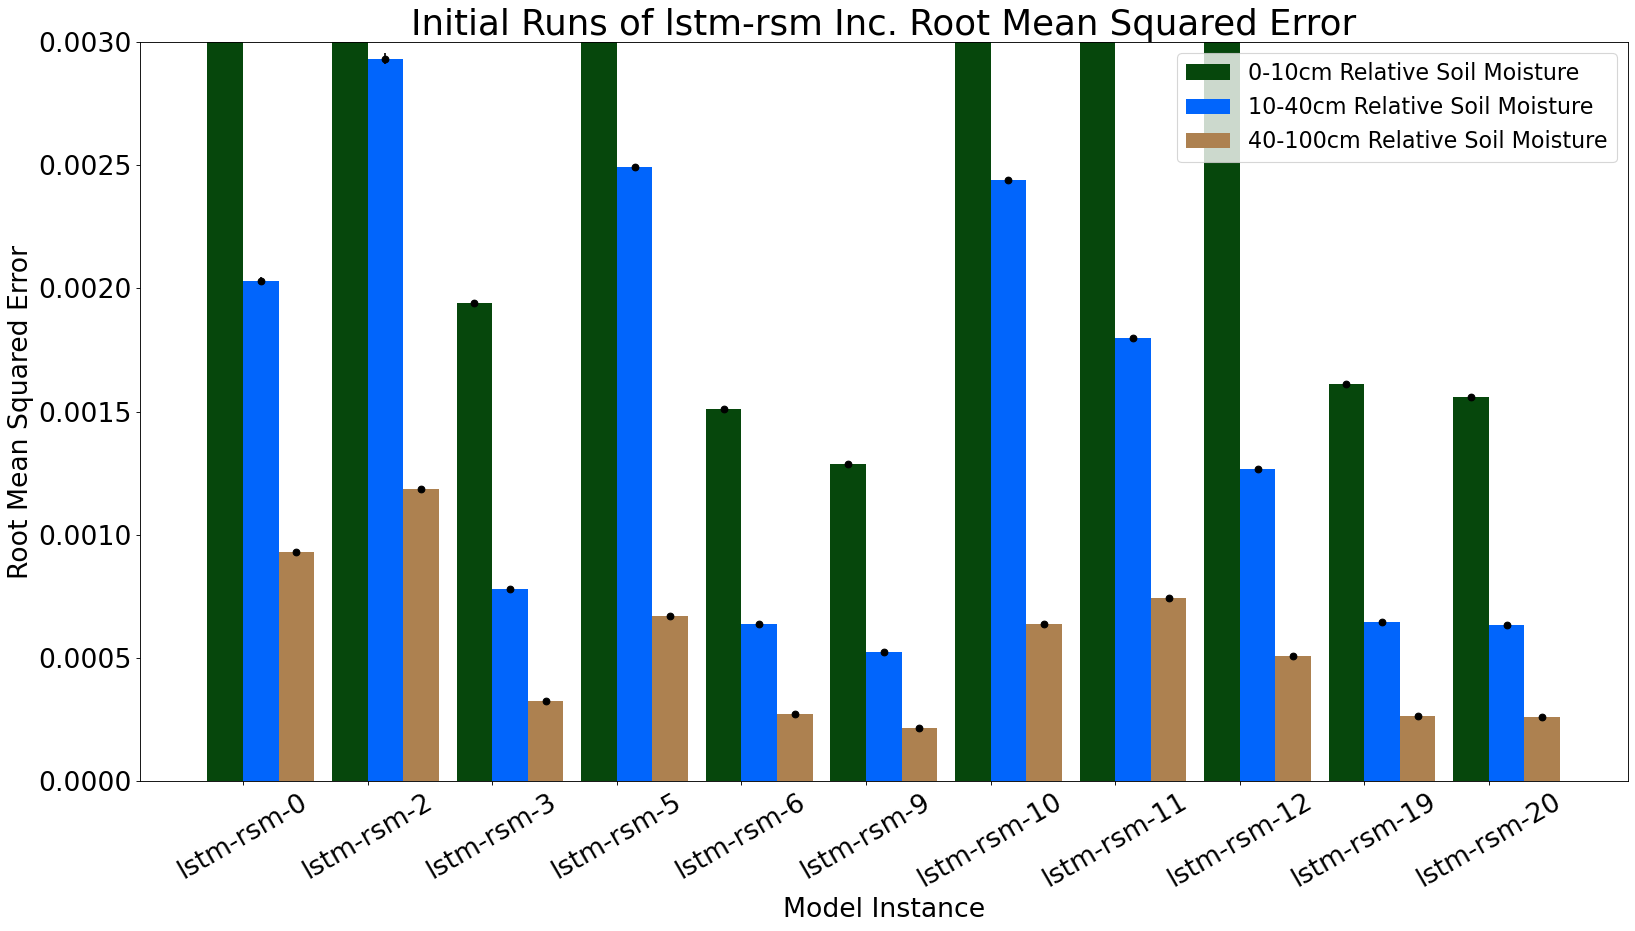
\includegraphics[width=.48\linewidth,draft=false]{figures/efficiency_initial-best/eval_test_efficiency_initial-lstm-rsm_mse_res.png}
    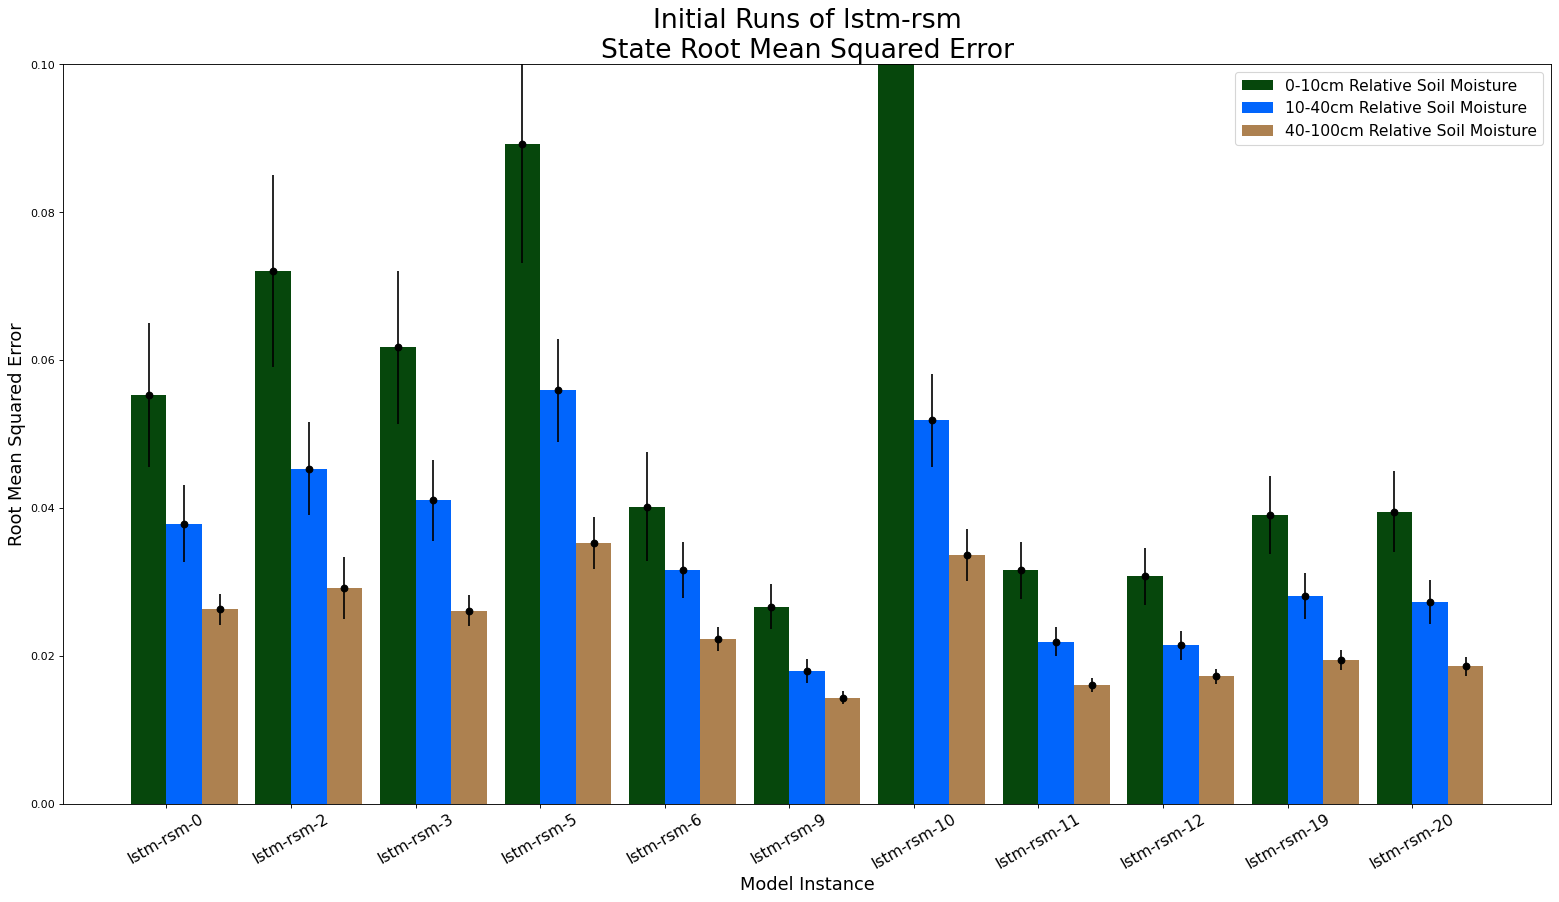
\includegraphics[width=.48\linewidth,draft=false]{figures/efficiency_initial-best/eval_test_efficiency_initial-lstm-rsm_mse_state.png}

    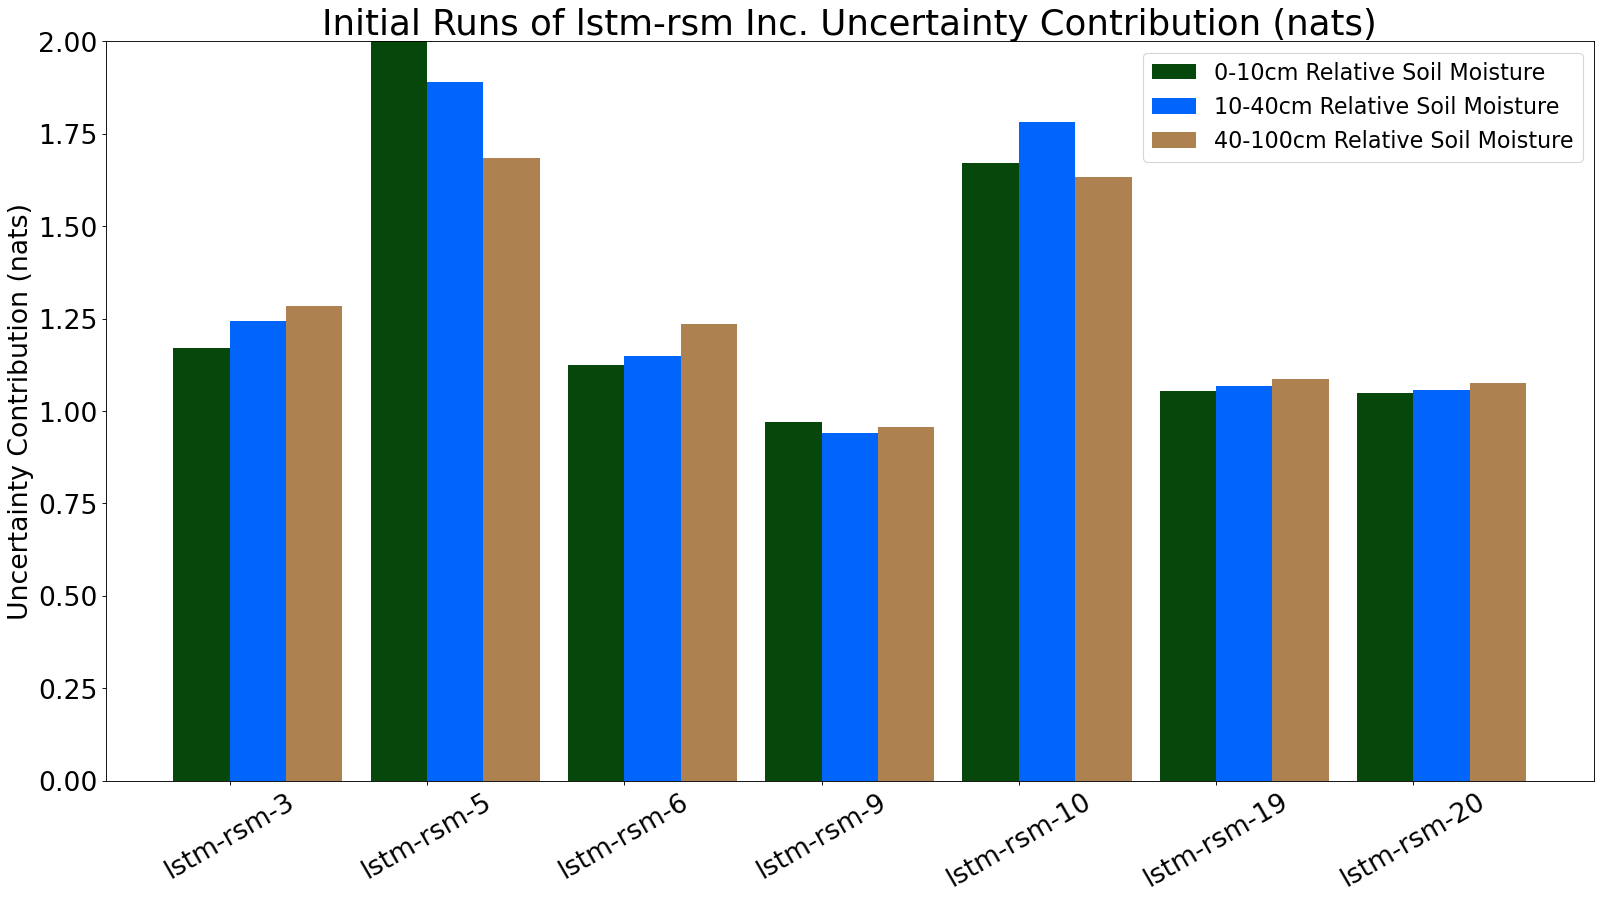
\includegraphics[width=.48\linewidth,draft=false]{figures/efficiency_initial-best/eval_test_efficiency_initial-lstm-rsm_info-loss_res.png}
    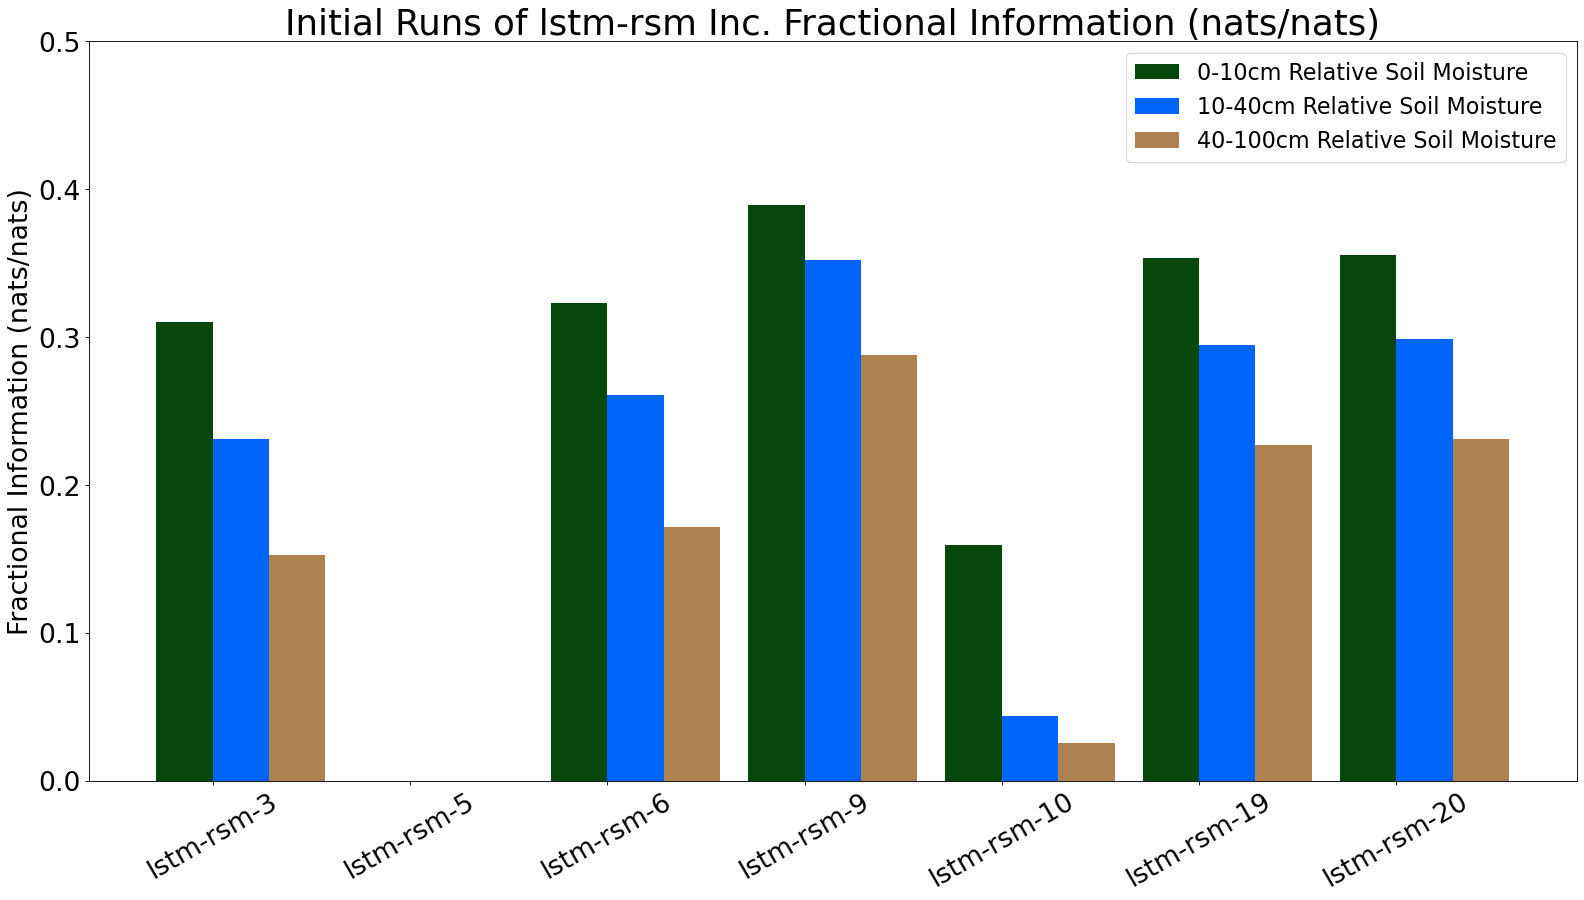
\includegraphics[width=.48\linewidth,draft=false]{figures/efficiency_initial-best/eval_test_efficiency_initial-lstm-rsm_fi_res.png}

    \caption{Bulk metrics for initial LSTM-RSM (relative soil moisture predictor) training runs}
    \label{model-init-lstm-rsm}
\end{figure}

\begin{table}[H]
\begin{sideways}
    \begin{tabular}{c|c|c|c|c|c|c }
    \small
Name & Desc & Weights & \thead{State\\MAE} & \thead{State\\CC} & \thead{Info\\Loss} &\thead{Frac.\\Info}\\
\hline
\multirow{3}{6em}{lstm-rsm-0} & \multirow{3}{16em}{Small magnitude bias. low dropout. small batch size. 64-wide 4-layer.} & \multirow{3}{4em}{179483} & 0.034 & 0.868 &  &  \\ & & & 0.021 & 0.837 &  &  \\ & & & 0.014 & 0.707 &  &  \\
\hline
\multirow{3}{6em}{lstm-rsm-2} & \multirow{3}{16em}{same as rsm-1, but some state error influence, magnitude bias 30} & \multirow{3}{4em}{179483} & 0.046 & 0.782 &  &  \\ & & & 0.026 & 0.761 &  &  \\ & & & 0.016 & 0.660 &  &  \\
\hline
\multirow{3}{6em}{lstm-rsm-3} & \multirow{3}{16em}{Low dropout, 4 deep, 64 wide decoder, and increment-only loss} & \multirow{3}{4em}{176379} & 0.039 & 0.861 & 1.169 & 0.310 \\ & & & 0.023 & 0.823 & 1.243 & 0.231 \\ & & & 0.015 & 0.677 & 1.285 & 0.152 \\
\hline
\multirow{3}{6em}{lstm-rsm-5} & \multirow{3}{16em}{Same as lstm-rsm-3, but 10\% state influence in loss function} & \multirow{3}{4em}{176379} & 0.057 & 0.133 & 2.206 & 0.000 \\ & & & 0.034 & 0.191 & 1.890 & 0.000 \\ & & & 0.020 & 0.205 & 1.686 & 0.000 \\
\hline
\multirow{3}{6em}{lstm-rsm-6} & \multirow{3}{16em}{Small 3-layer predictor with 100 increment magnitude bias} & \multirow{3}{4em}{48667} & 0.023 & 0.886 & 1.124 & 0.323 \\ & & & 0.017 & 0.805 & 1.149 & 0.261 \\ & & & 0.012 & 0.723 & 1.235 & 0.171 \\
\hline
\multirow{3}{6em}{lstm-rsm-9} & \multirow{3}{16em}{32 nodes wide, 4 layers deep, 10 increment magnitude bias} & \multirow{3}{4em}{48667} & 0.015 & 0.932 & 0.970 & 0.389 \\ & & & 0.009 & 0.922 & 0.941 & 0.352 \\ & & & 0.007 & 0.877 & 0.958 & 0.288 \\
\hline
\multirow{3}{6em}{lstm-rsm-10} & \multirow{3}{16em}{256 nodes wide 5-layer model} & \multirow{3}{4em}{2614907} & 0.138 & 0.168 & 1.671 & 0.159 \\ & & & 0.031 & 0.537 & 1.783 & 0.044 \\ & & & 0.019 & 0.534 & 1.632 & 0.025 \\
%\multirow{3}{6em}{lstm-rsm-11} & \multirow{3}{16em}{same as rsm-9 except coarsened to 3h predictions} & \multirow{3}{4em}{79675} & 0.018 & 0.904 &  &  \\ & & & 0.012 & 0.897 &  &  \\ & & & 0.009 & 0.844 &  &  \\
\hline
\multirow{3}{6em}{lstm-rsm-12} & \multirow{3}{16em}{4 layers deep, 32 nodes wide, steep learning rate decay} & \multirow{3}{4em}{78651} & 0.017 & 0.912 &  &  \\ & & & 0.011 & 0.904 &  &  \\ & & & 0.009 & 0.833 &  &  \\
\hline
\multirow{3}{6em}{lstm-rsm-19} & \multirow{3}{16em}{Single layer 256 nodes wide} & \multirow{3}{4em}{725627} & 0.022 & 0.899 & 1.055 & 0.353 \\ & & & 0.015 & 0.850 & 1.067 & 0.295 \\ & & & 0.010 & 0.806 & 1.086 & 0.227 \\
\hline
\multirow{3}{6em}{lstm-rsm-20} & \multirow{3}{16em}{Same as rsm-19 except some influence of state error} & \multirow{3}{4em}{725627} & 0.023 & 0.899 & 1.048 & 0.356 \\ & & & 0.014 & 0.852 & 1.058 & 0.299 \\ & & & 0.010 & 0.803 & 1.075 & 0.231 \\
    \end{tabular}
\centering
\end{sideways}
    \caption{Initial RSM-normalized LSTM properties and bulk statistics.}
\end{table}

The next group of models we trained will be referred to as LSTM-RSM models, which have the same structure as the previous set, but target the increment change in RSM rather than volumetric soil moisture. Like the LSTM-SOILM models, these seemed to show diminishing returns with model sizes beyond 100,000 weights. The best model we identified has only 48,667 trainable weights, and is 4 layers in depth. Curiously, while the loss function manipulations appeared to have a positive impact on the FNN and LSTM-SOILM variants, LSTM-RSM models generally underperformed when a higher magnitude bias and a stronger contribution from the state were used. The best model had a relatively small increment magnitude bias $\gamma=10$, and no contribution from state error ($\rho=1$).


%\begin{figure}[hp!]
%    \centering
%    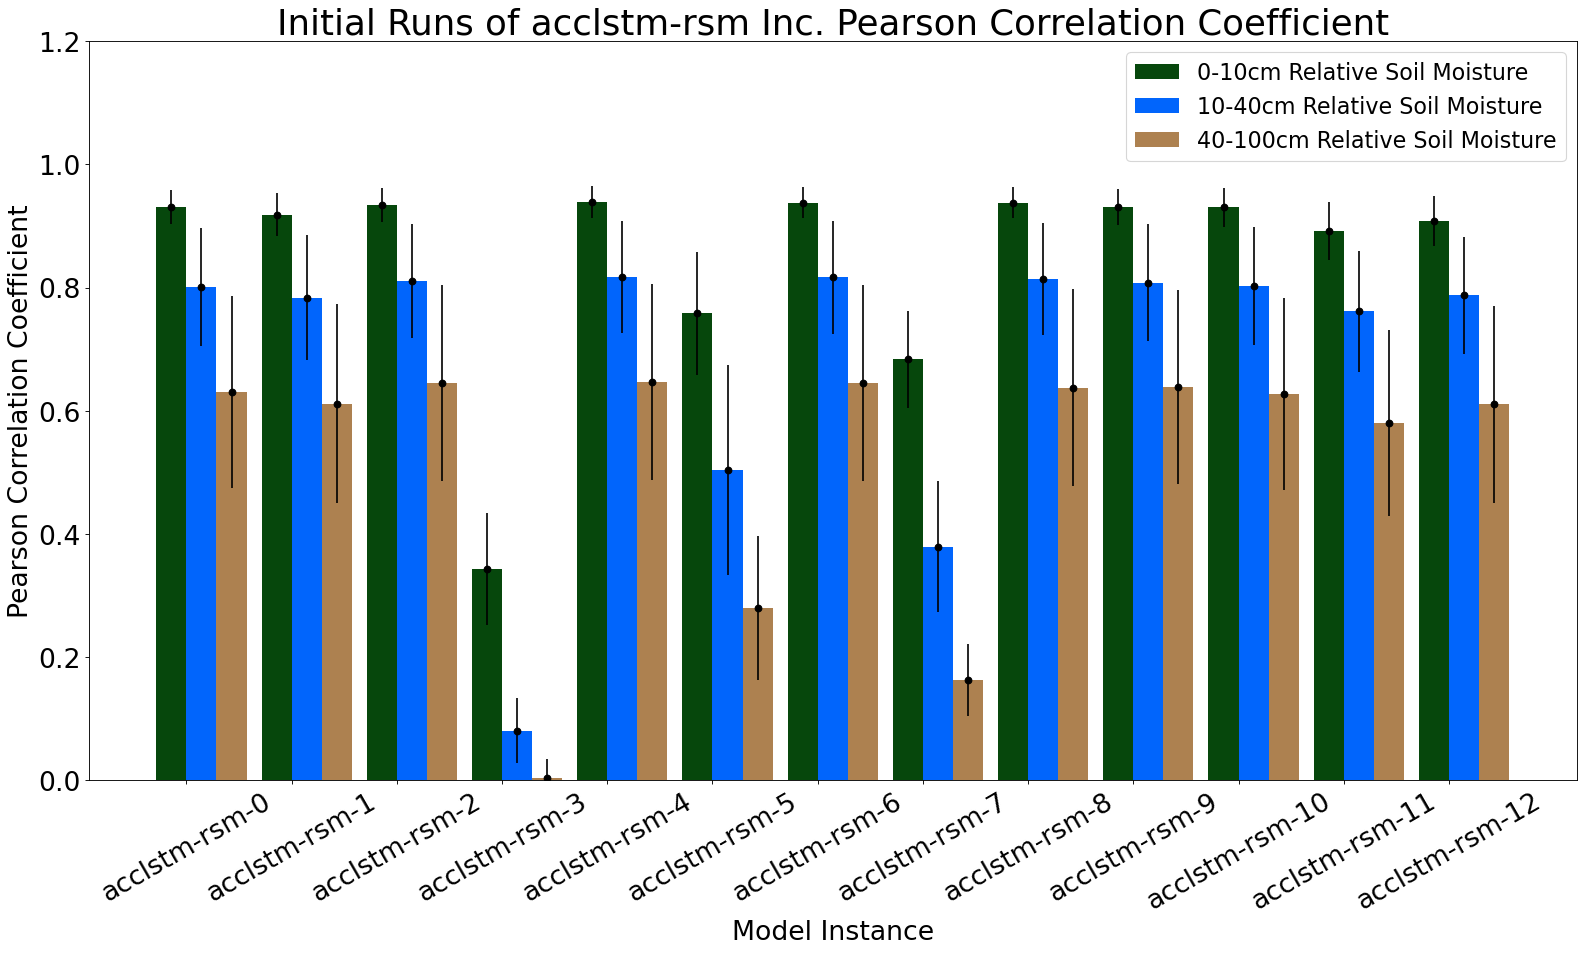
\includegraphics[width=.48\linewidth,draft=false]{figures/efficiency_initial-best/eval_test_efficiency_initial-acclstm-rsm_cc_res.png}
%    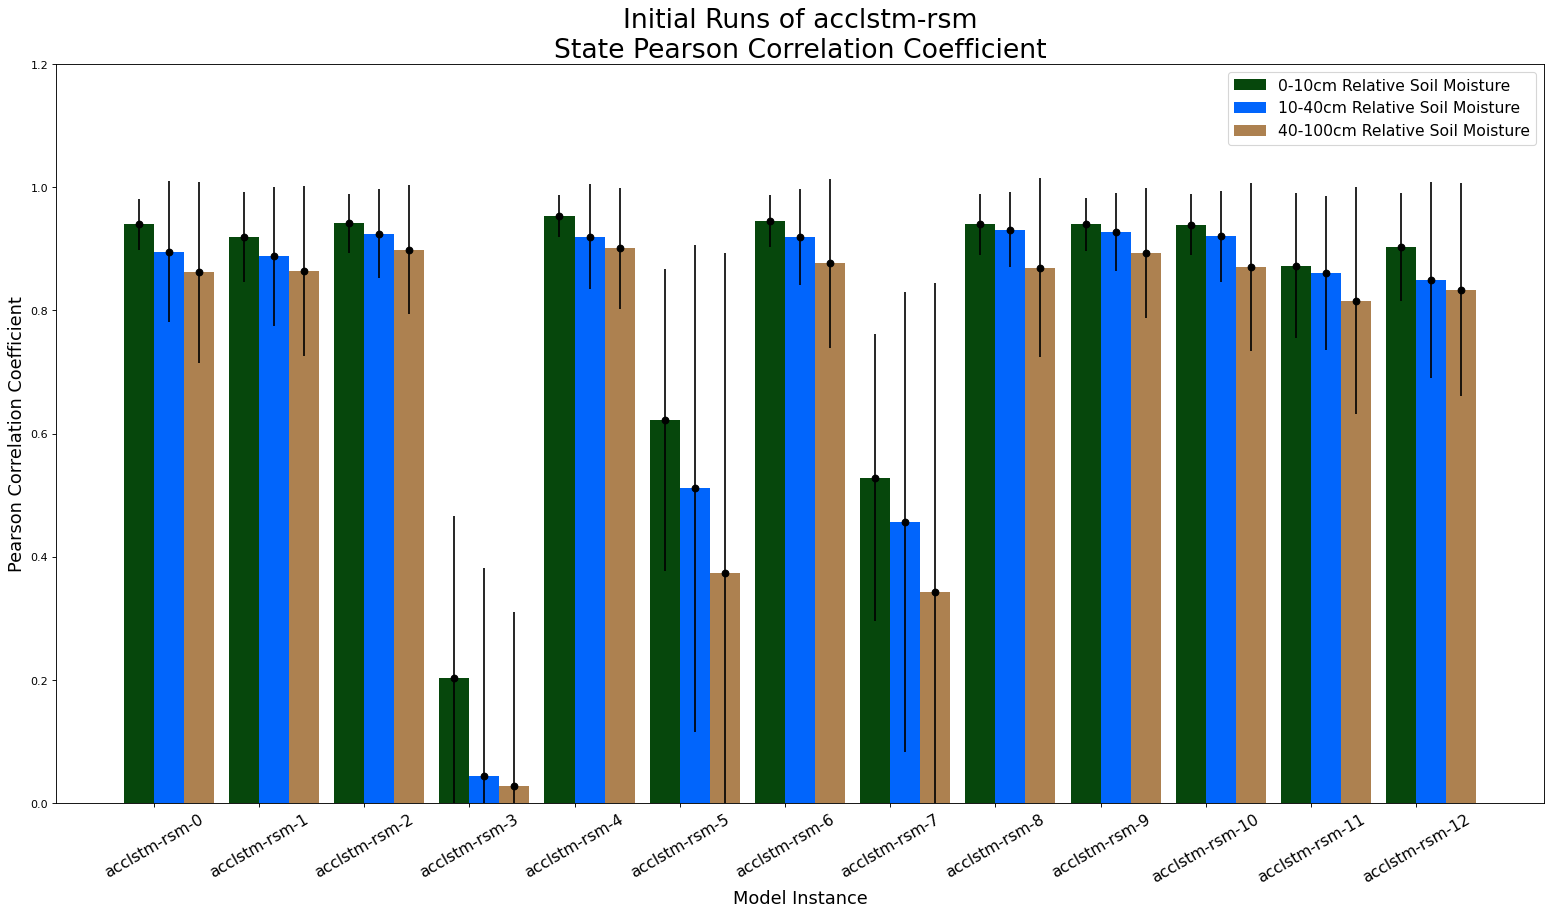
\includegraphics[width=.48\linewidth,draft=false]{figures/efficiency_initial-best/eval_test_efficiency_initial-acclstm-rsm_cc_state.png}
%
%    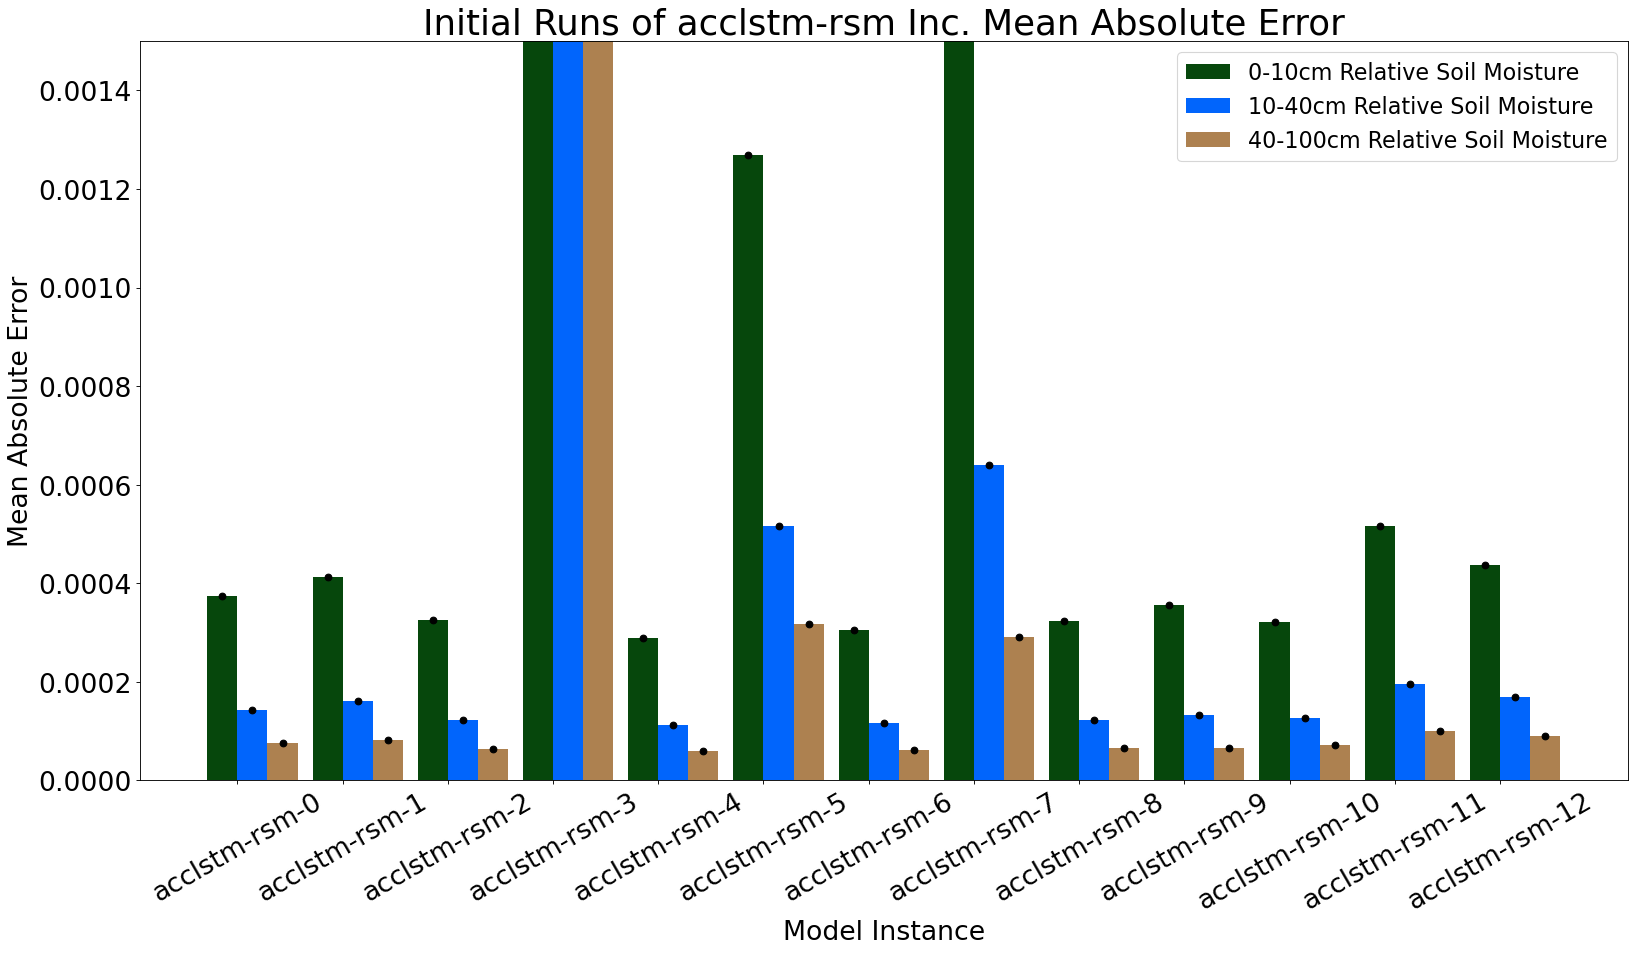
\includegraphics[width=.48\linewidth,draft=false]{figures/efficiency_initial-best/eval_test_efficiency_initial-acclstm-rsm_mae_res.png}
%    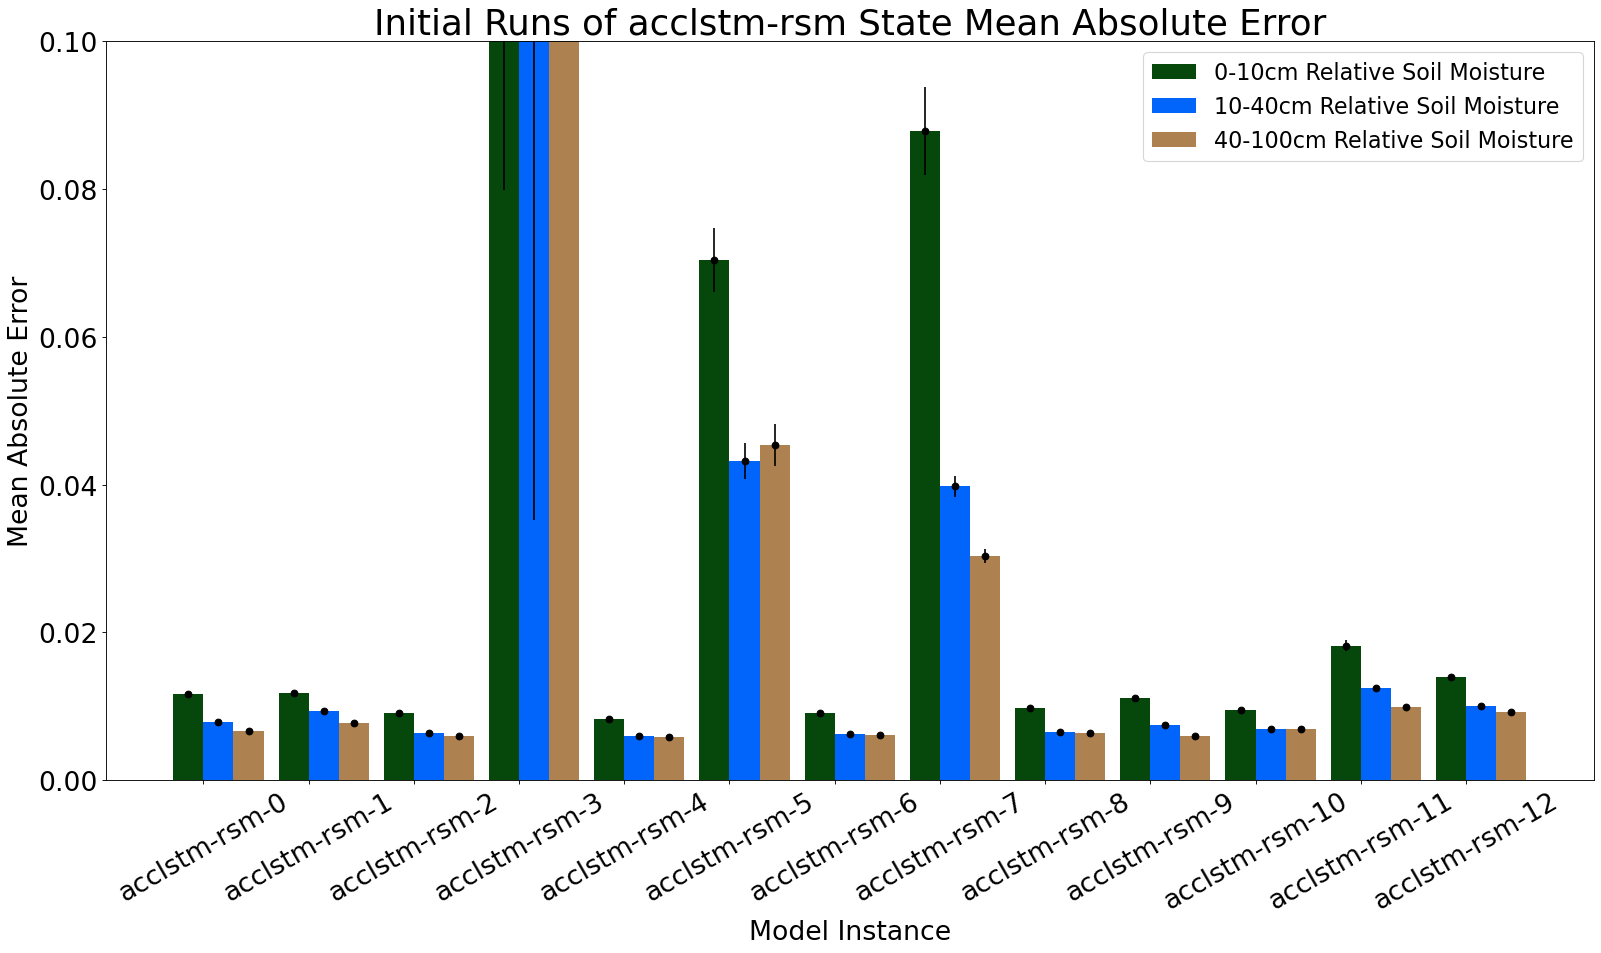
\includegraphics[width=.48\linewidth,draft=false]{figures/efficiency_initial-best/eval_test_efficiency_initial-acclstm-rsm_mae_state.png}
%
%    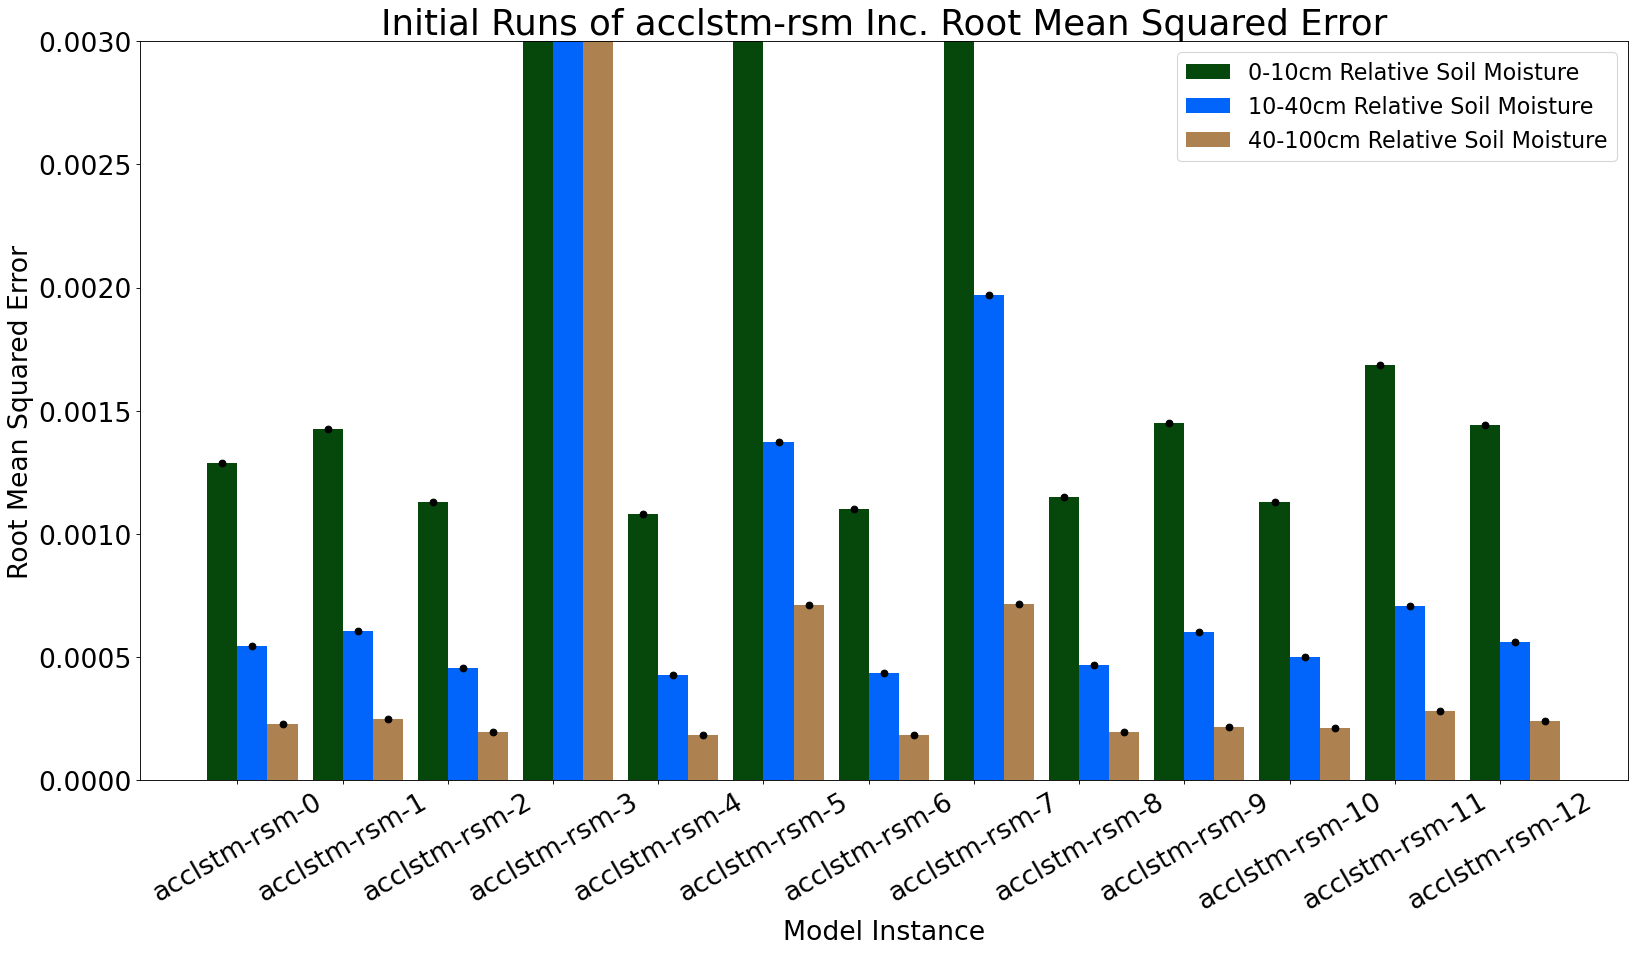
\includegraphics[width=.48\linewidth,draft=false]{figures/efficiency_initial-best/eval_test_efficiency_initial-acclstm-rsm_mse_res.png}
%    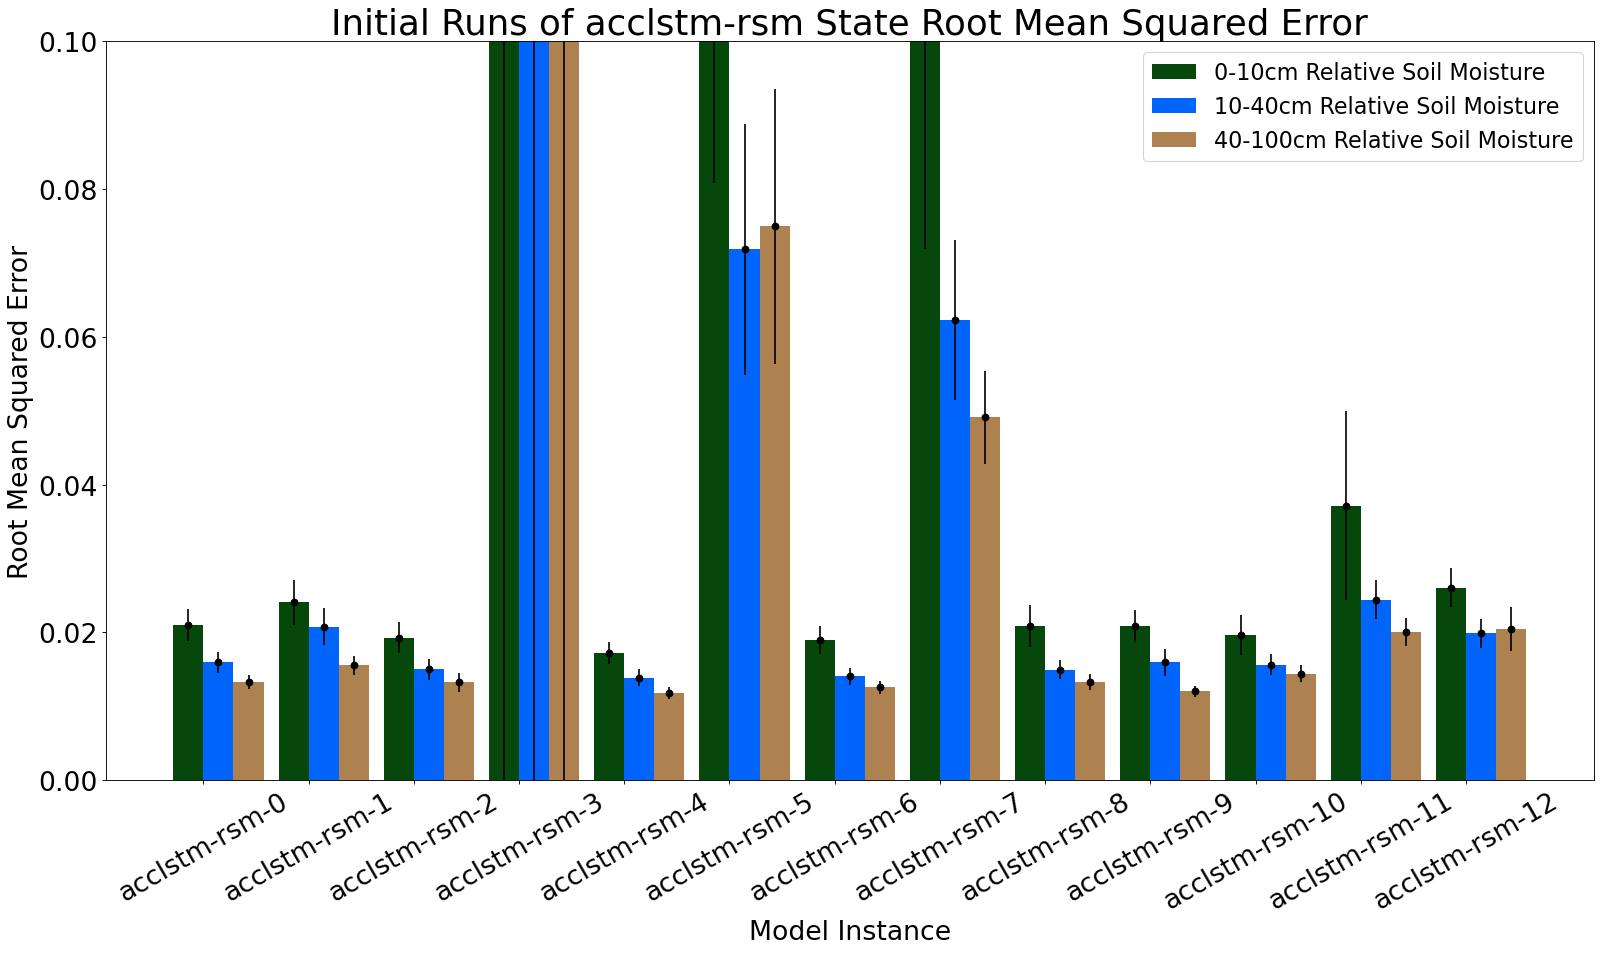
\includegraphics[width=.48\linewidth,draft=false]{figures/efficiency_initial-best/eval_test_efficiency_initial-acclstm-rsm_mse_state.png}
%
%    \caption{Bulk metrics for initial AccLSTM-RSM training runs}
%    \label{model-init-acclstm-rsm}
%\end{figure}
%
%\begin{sidewaystable}
%\begin{center}
%    \begin{tabular}{c|c|c|c|c|c|c }
%    \end{tabular}
%\end{center}
%\end{sidewaystable}


\section{Best Models' Bulk Statistics Comparison}

\begin{figure}[hp!]
    \centering
    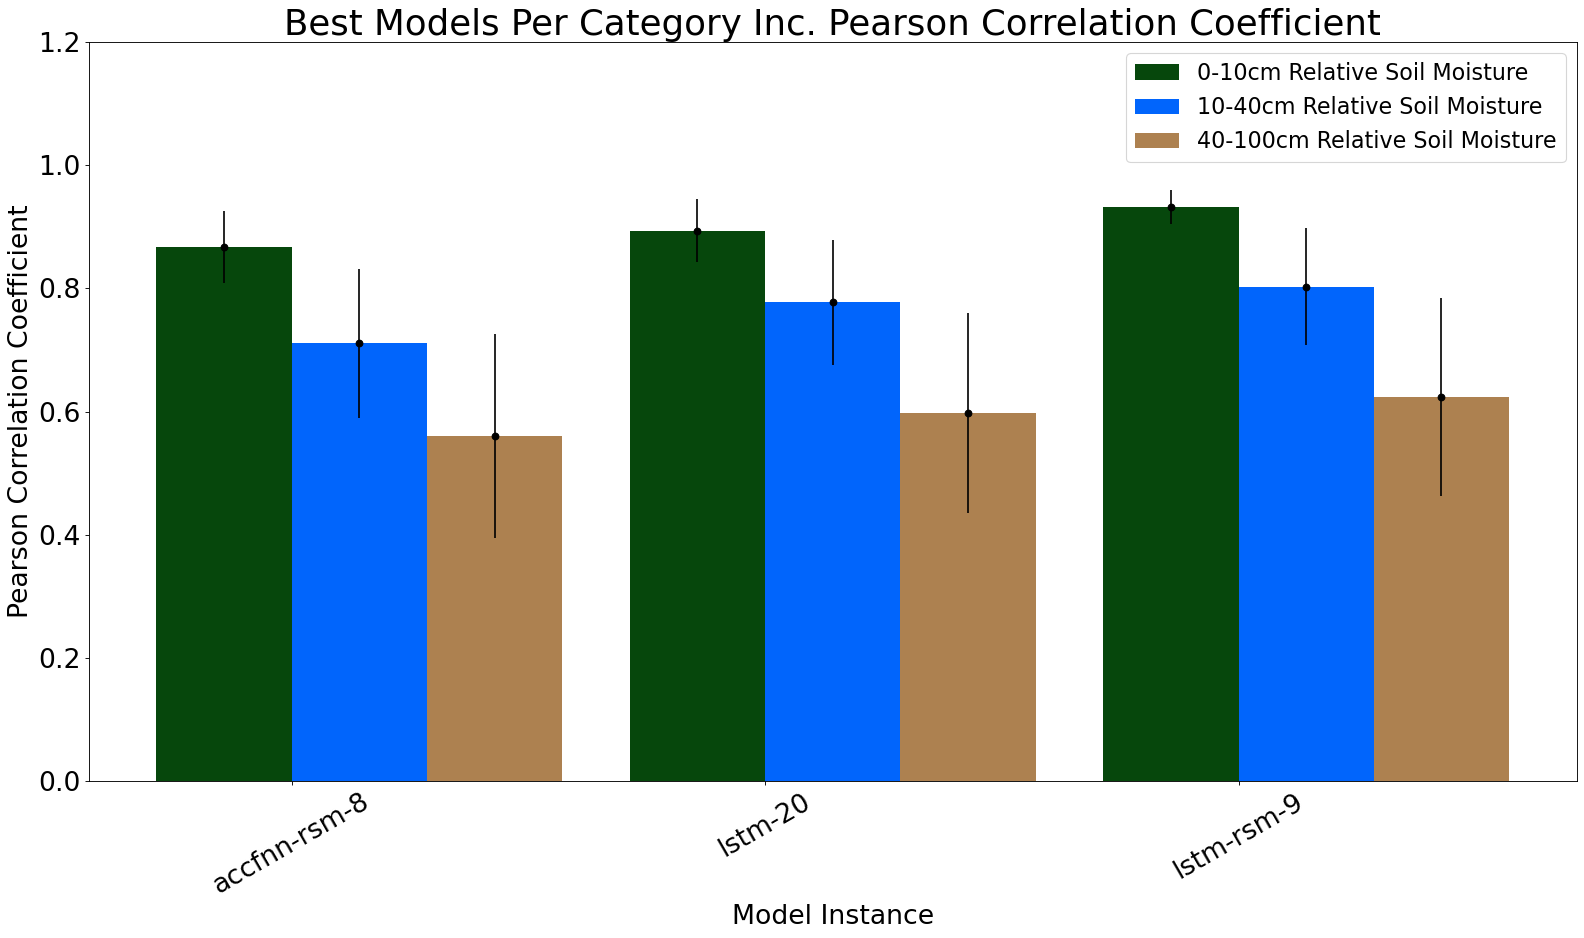
\includegraphics[width=.48\linewidth,draft=false]{figures/efficiency_initial-best/eval_test_efficiency_initial-best_cc_res.png}
    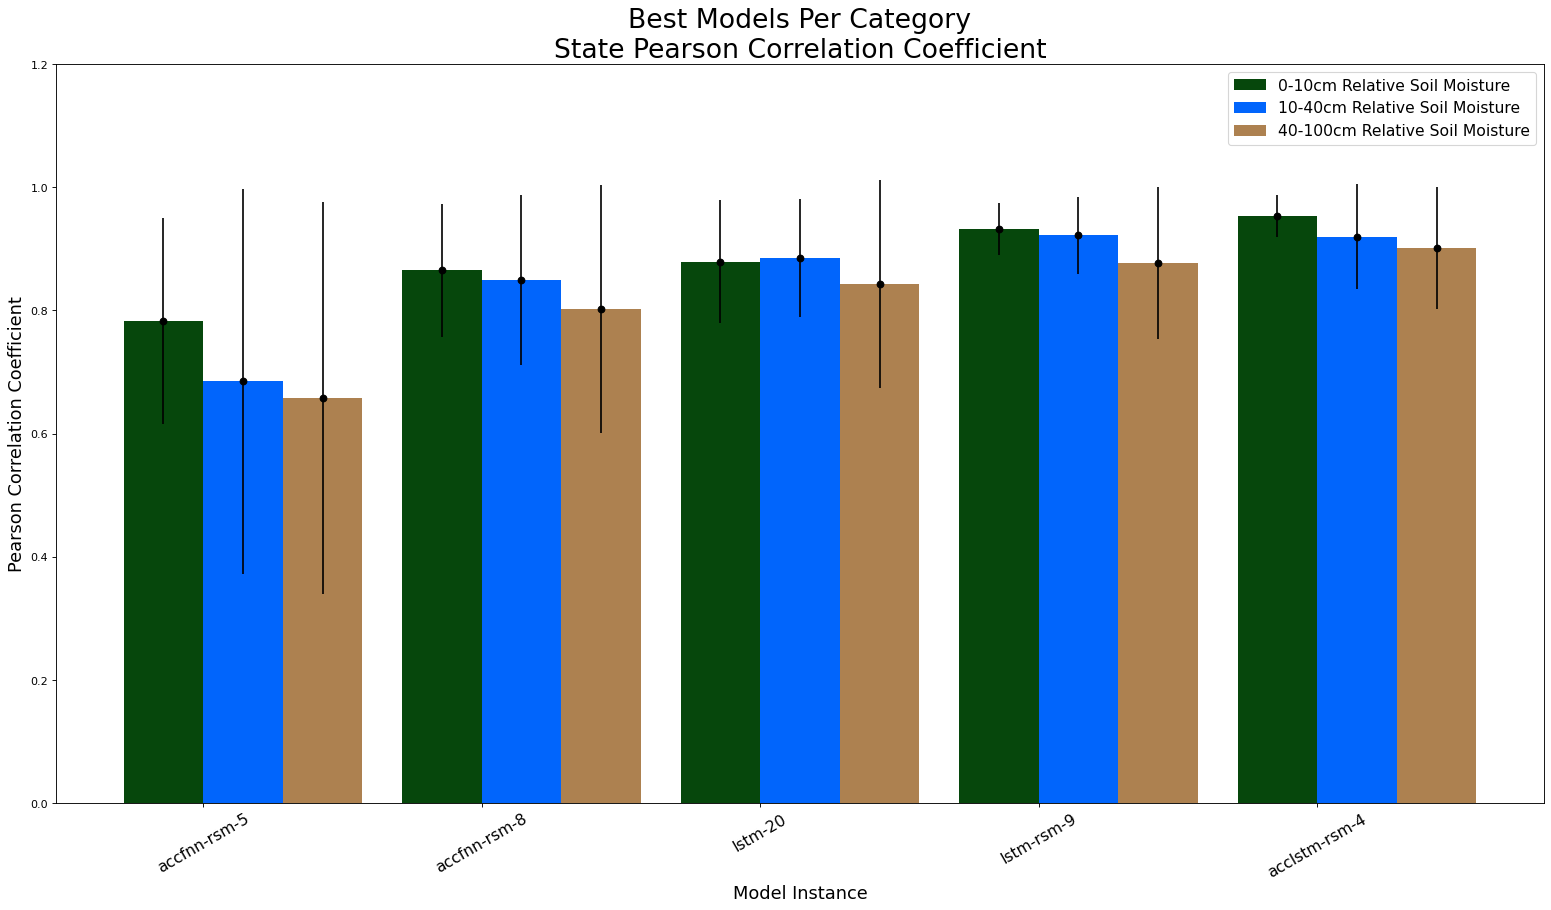
\includegraphics[width=.48\linewidth,draft=false]{figures/efficiency_initial-best/eval_test_efficiency_initial-best_cc_state.png}

    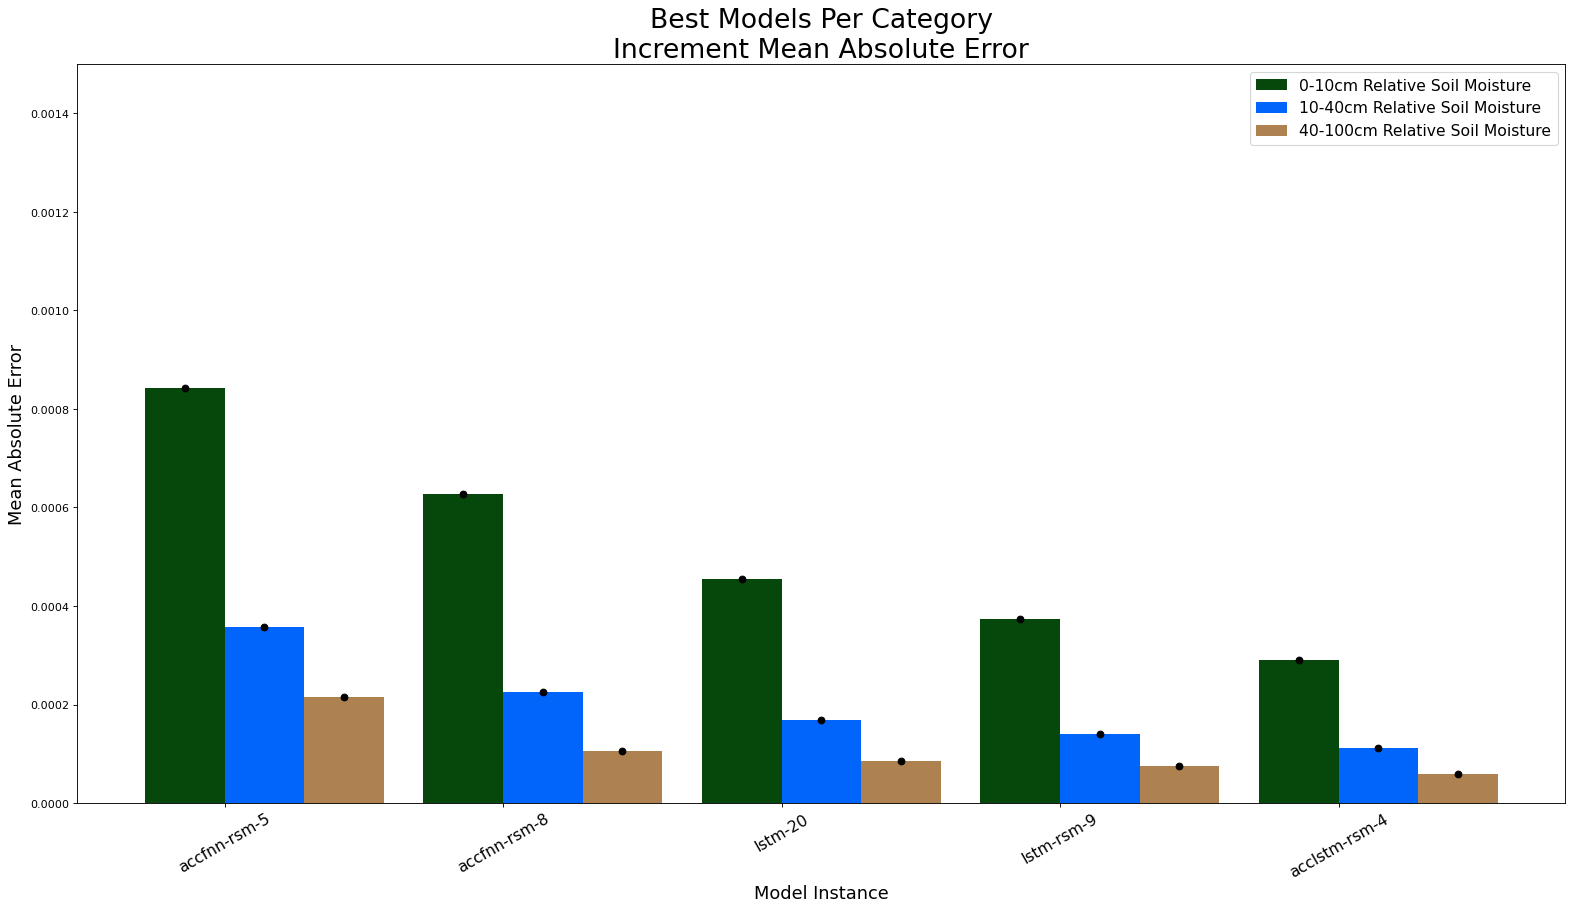
\includegraphics[width=.48\linewidth,draft=false]{figures/efficiency_initial-best/eval_test_efficiency_initial-best_mae_res.png}
    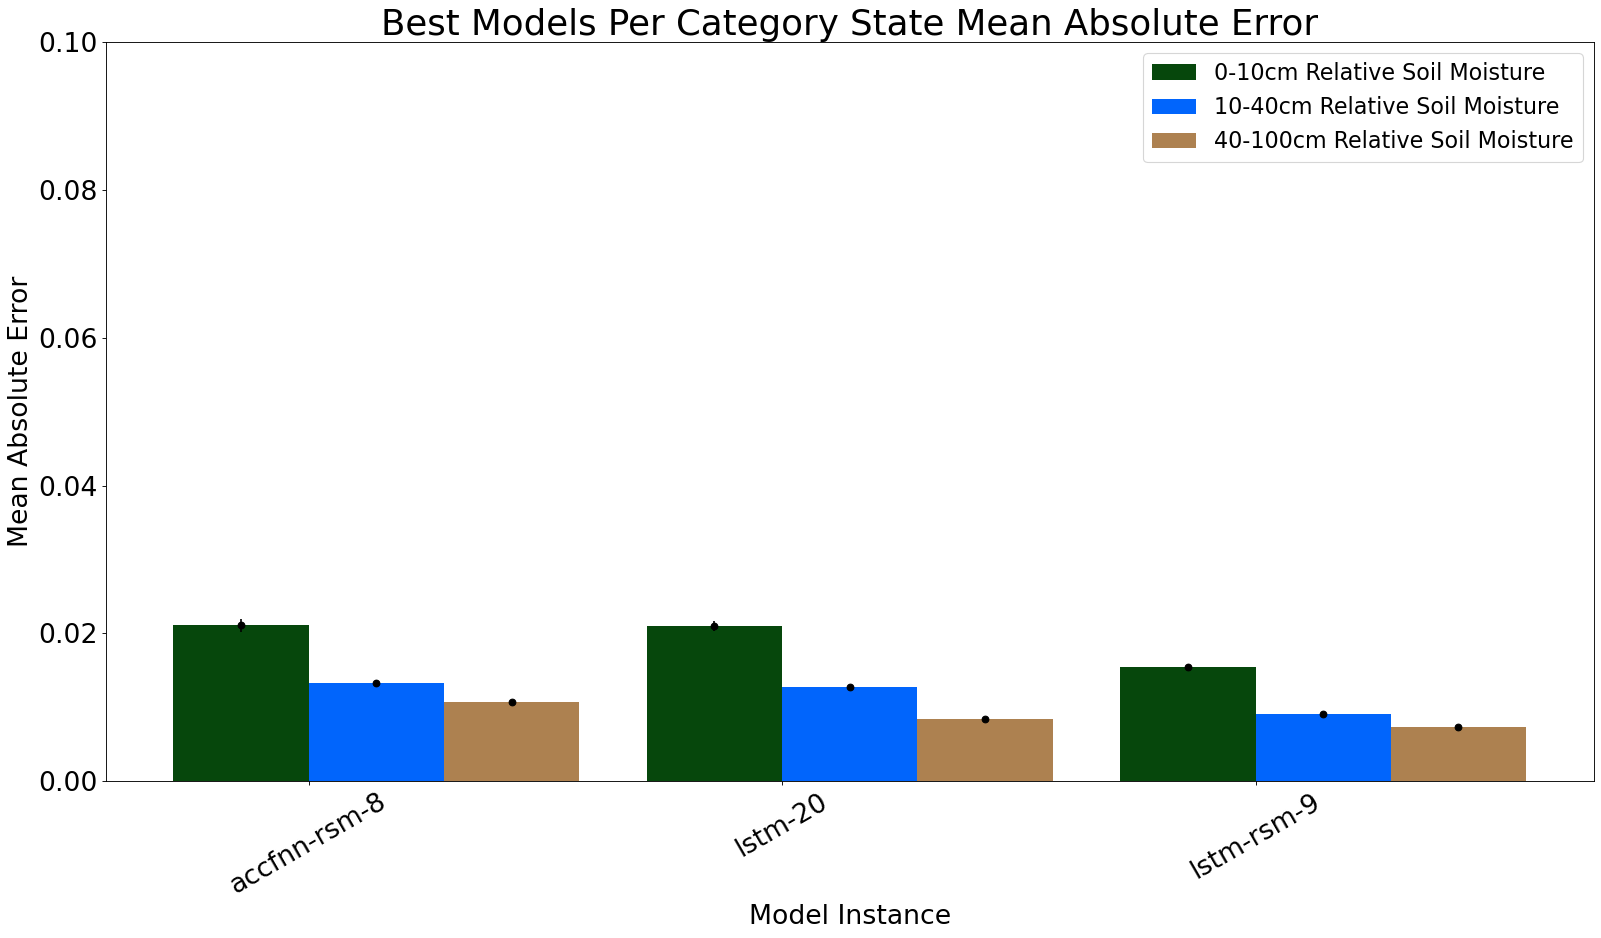
\includegraphics[width=.48\linewidth,draft=false]{figures/efficiency_initial-best/eval_test_efficiency_initial-best_mae_state.png}

    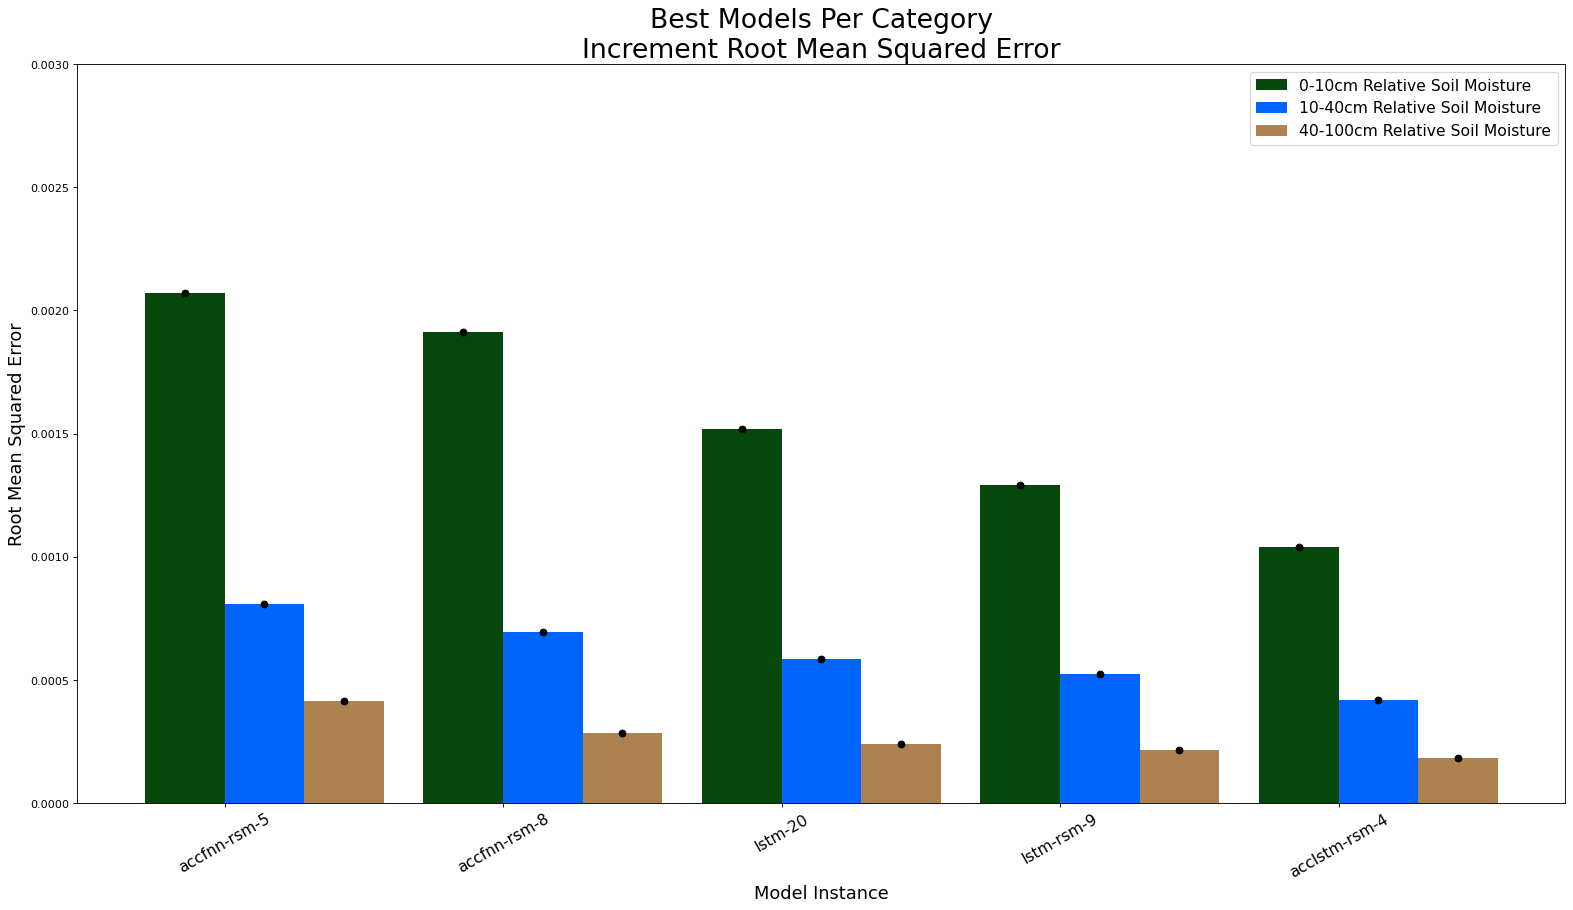
\includegraphics[width=.48\linewidth,draft=false]{figures/efficiency_initial-best/eval_test_efficiency_initial-best_mse_res.png}
    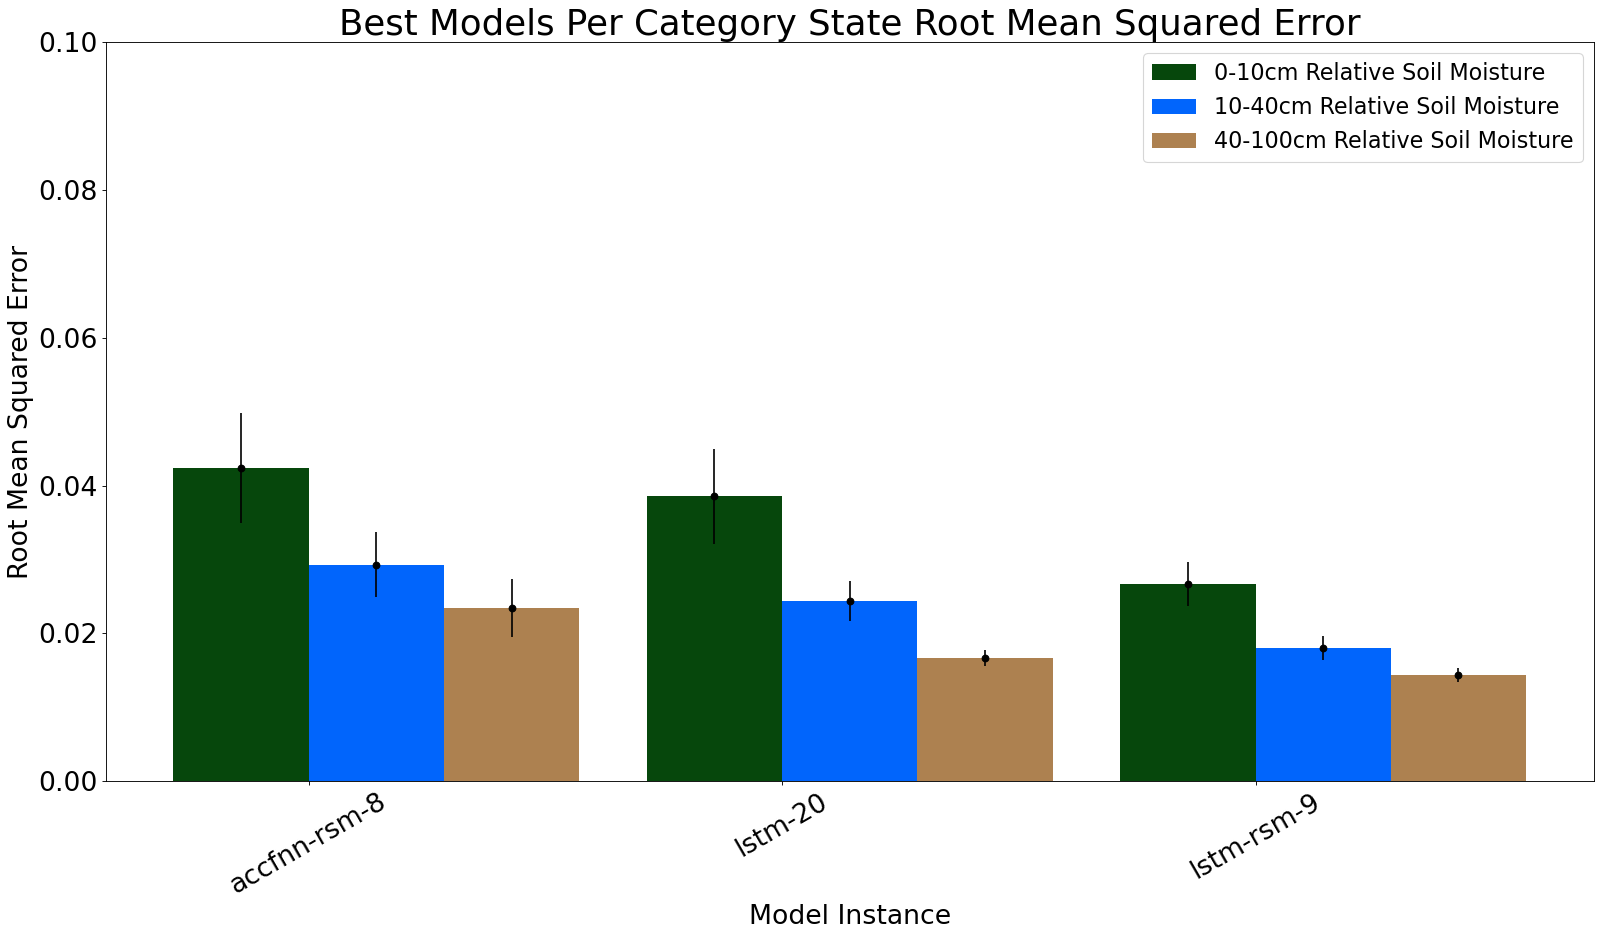
\includegraphics[width=.48\linewidth,draft=false]{figures/efficiency_initial-best/eval_test_efficiency_initial-best_mse_state.png}

    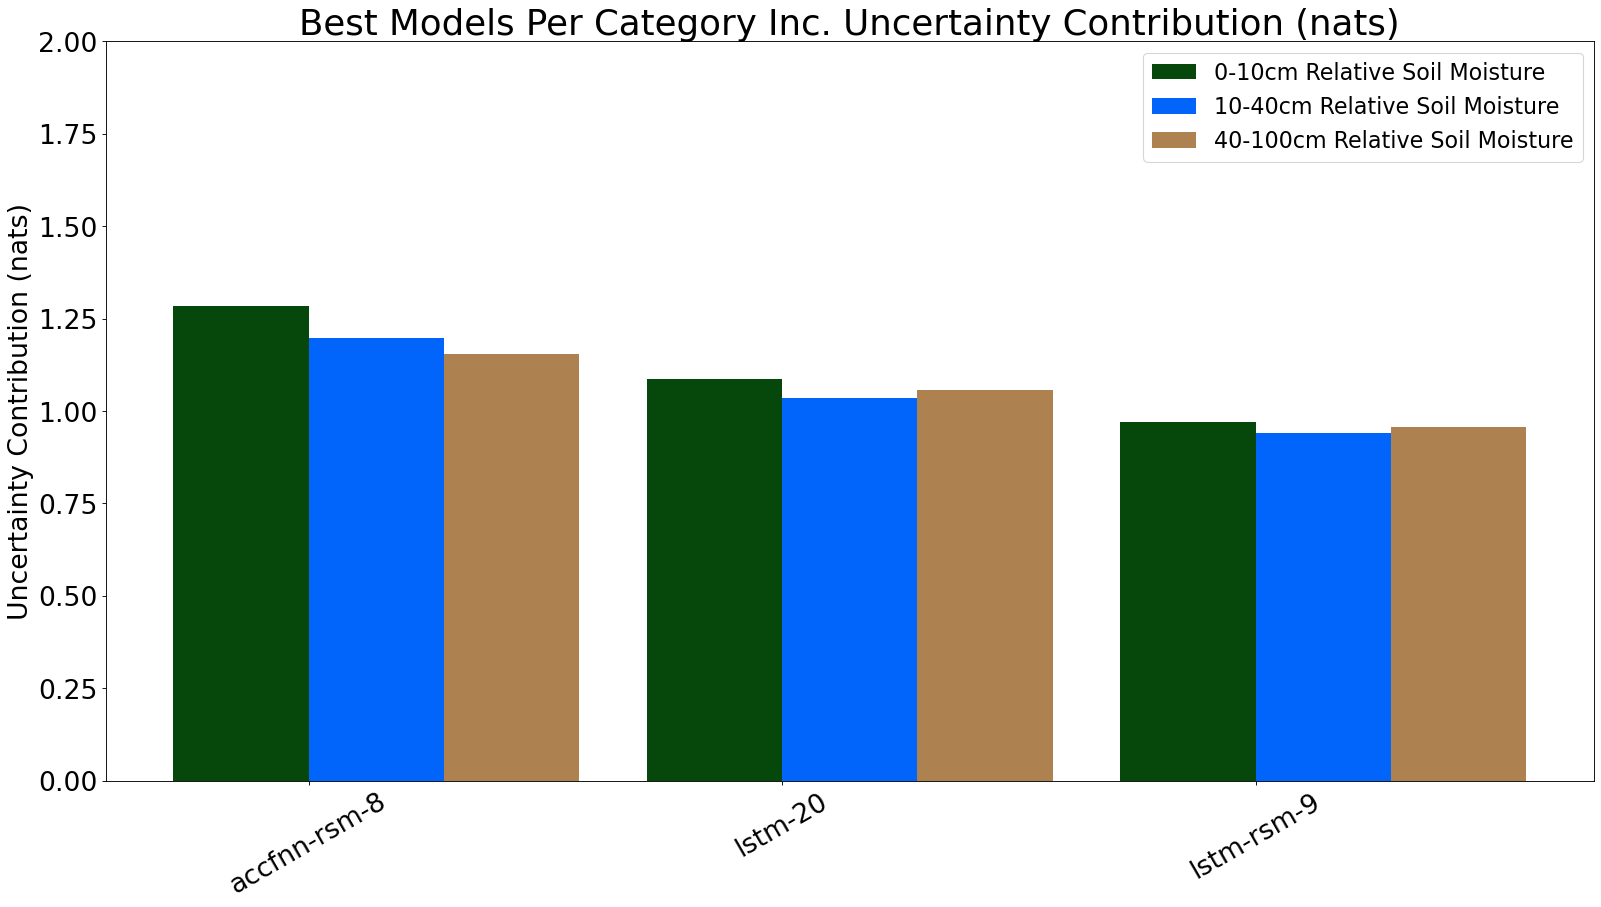
\includegraphics[width=.48\linewidth,draft=false]{figures/efficiency_initial-best/eval_test_efficiency_initial-best_info-loss_res.png}
    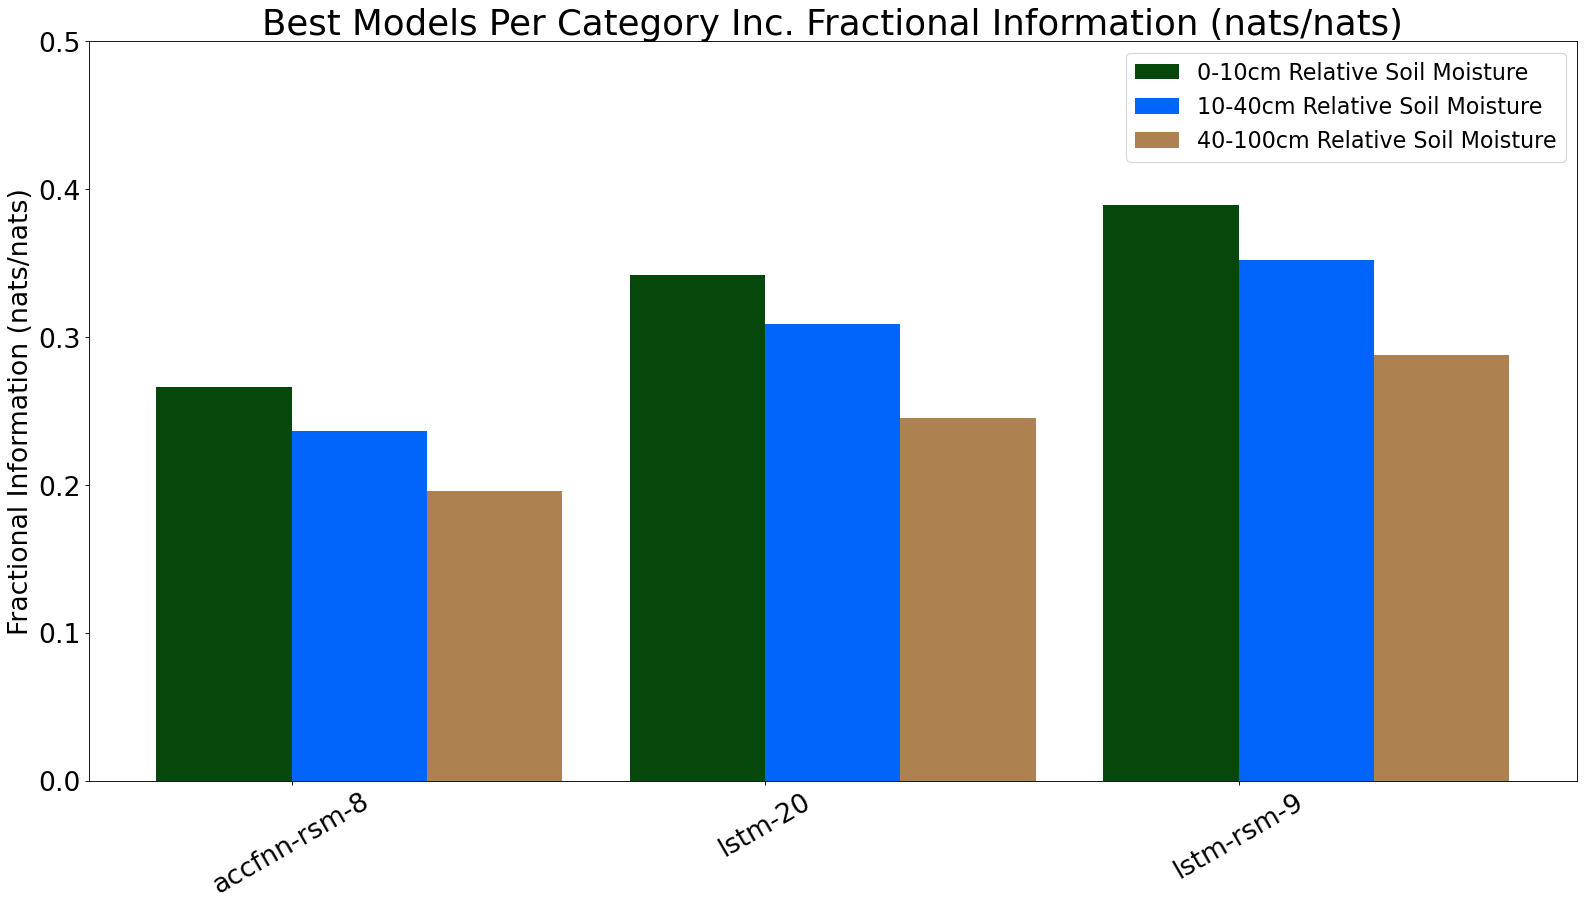
\includegraphics[width=.48\linewidth,draft=false]{figures/efficiency_initial-best/eval_test_efficiency_initial-best_fi_res.png}

    \caption{Bulk metrics comparing the best exploratory models from each category}
    \label{best-metrics}
\end{figure}

\begin{table}[H]
    \centering
    \begin{tabular}{c|c|c|c|c }
        Name & Slope ($ms$) & Intercept ($\frac{s}{px}$) & R$^2$ & Full Domain ($s$) \\
        \hline
        accfnn-rsm-8 & .1262 & 3.088 & .852 & 9.508 \\
        lstm-20 & .8233 & 3.510 & .984 & 45.397 \\
        lstm-rsm-9 & .7544 & 3.246 & .953 & 41.627 \\
    \end{tabular}
    \label{best-exec-efficiency-table}
    \caption{Linear regression of execution speed for each of the best models.}
\end{table}

\begin{table}[H]
    \centering
    \begin{tabular}{c|c|c|c|c|c}
Name &  Weights & \thead{State\\MAE} & \thead{State\\CC} & \thead{Info\\Loss} &\thead{Frac.\\Info}\\
\hline
\multirow{3}{6em}{accfnn-rsm-8} &  \multirow{3}{4em}{30843} & 0.021 & 0.867 & 1.283 & 0.266 \\ & & 0.013 & 0.850 & 1.197 & 0.236 \\ & & 0.011 & 0.809 & 1.154 & 0.196 \\
\hline
\multirow{3}{6em}{lstm-20} &  \multirow{3}{4em}{77117} & 0.021 & 0.882 & 1.088 & 0.342 \\ & & 0.013 & 0.884 & 1.036 & 0.309 \\ & & 0.008 & 0.842 & 1.058 & 0.246 \\
\hline
\multirow{3}{6em}{lstm-rsm-9} & \multirow{3}{4em}{48667} & 0.015 & 0.932 & 0.970 & 0.389 \\ & & 0.009 & 0.922 & 0.941 & 0.352 \\ & & 0.007 & 0.877 & 0.958 & 0.288 \\
    \end{tabular}
\end{table}

\begin{figure}[hp!]
    \centering

    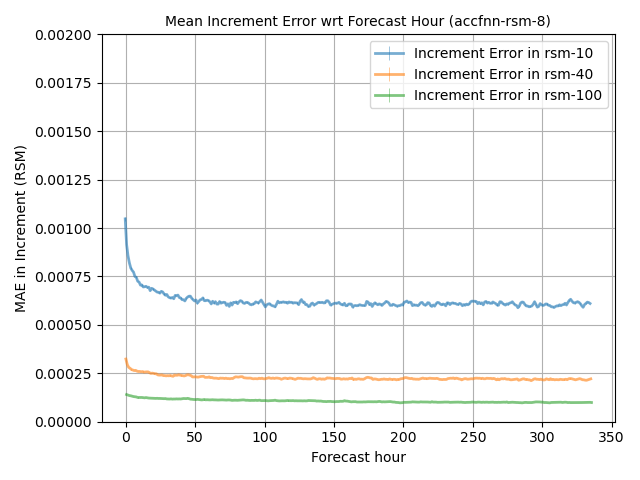
\includegraphics[width=.42\linewidth,draft=false]{figures/horizons/eval_test_accfnn-rsm-8_rsm_horizon_na_res.png}
    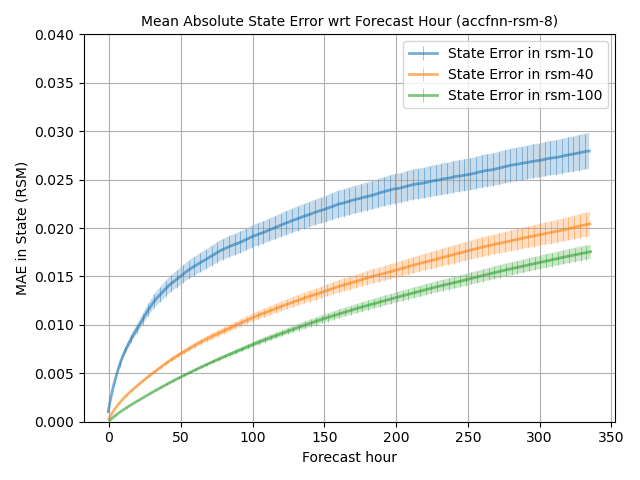
\includegraphics[width=.42\linewidth,draft=false]{figures/horizons/eval_test_accfnn-rsm-8_rsm_horizon_na_state.png}

    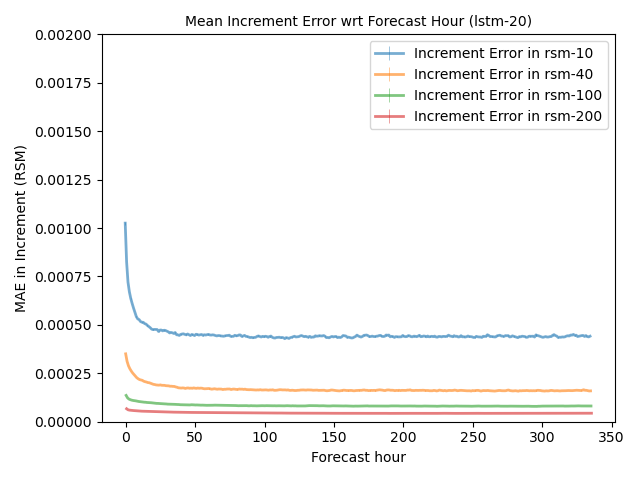
\includegraphics[width=.42\linewidth,draft=false]{figures/horizons/eval_test_lstm-20_rsm_horizon_na_res.png}
    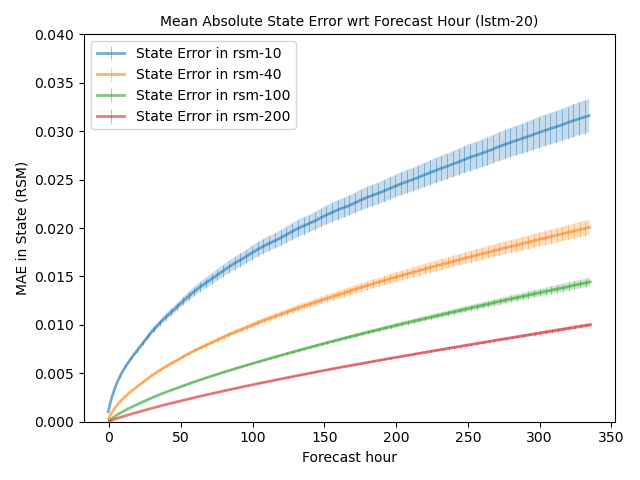
\includegraphics[width=.42\linewidth,draft=false]{figures/horizons/eval_test_lstm-20_rsm_horizon_na_state.png}

    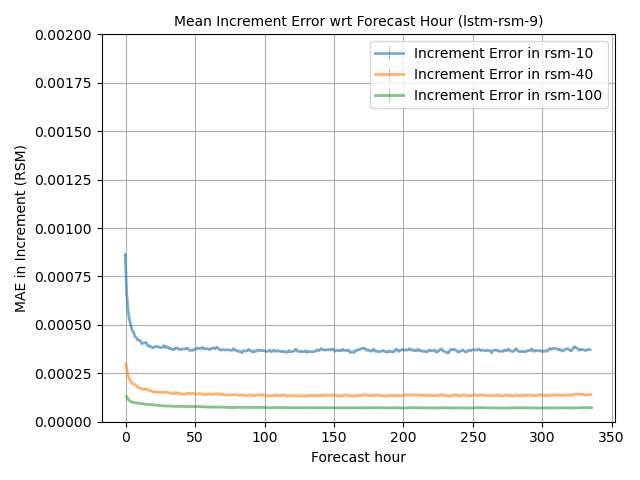
\includegraphics[width=.42\linewidth,draft=false]{figures/horizons/eval_test_lstm-rsm-9_rsm_horizon_na_res.png}
    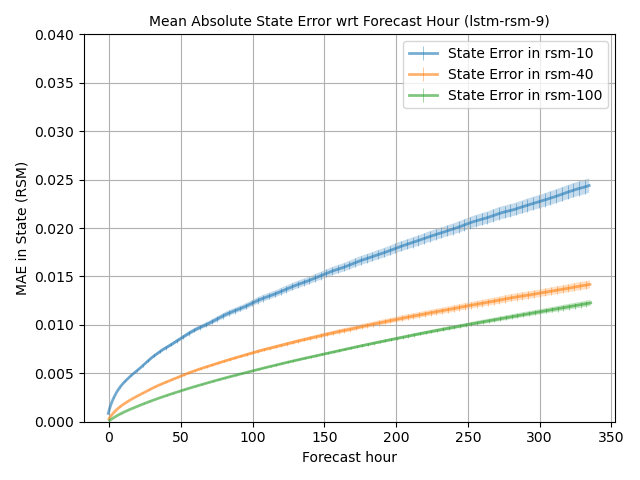
\includegraphics[width=.42\linewidth,draft=false]{figures/horizons/eval_test_lstm-rsm-9_rsm_horizon_na_state.png}

    %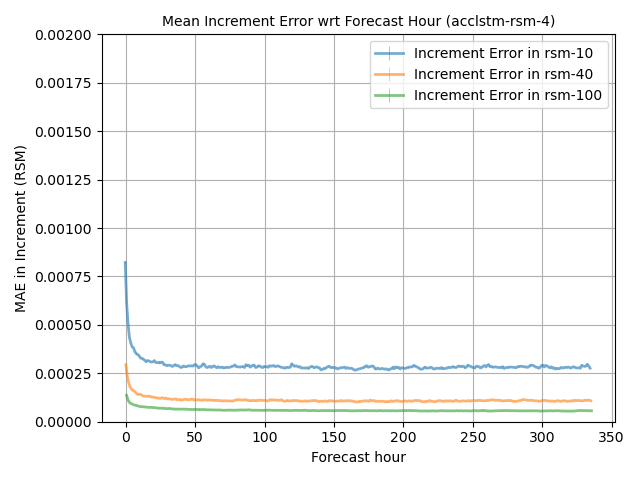
\includegraphics[width=.42\linewidth,draft=false]{figures/horizons/eval_test_acclstm-rsm-4_rsm_horizon_na_res.png}
    %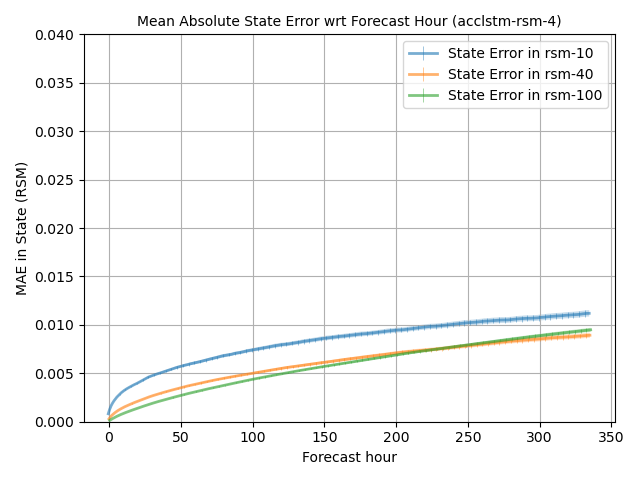
\includegraphics[width=.42\linewidth,draft=false]{figures/horizons/eval_test_acclstm-rsm-4_rsm_horizon_na_state.png}

    \caption{Mean absolute error of each model type with respect to forecast horizon increment (left) and state (right)}
    \label{best-horizons}
\end{figure}

\begin{figure}[hp!]
    \centering

    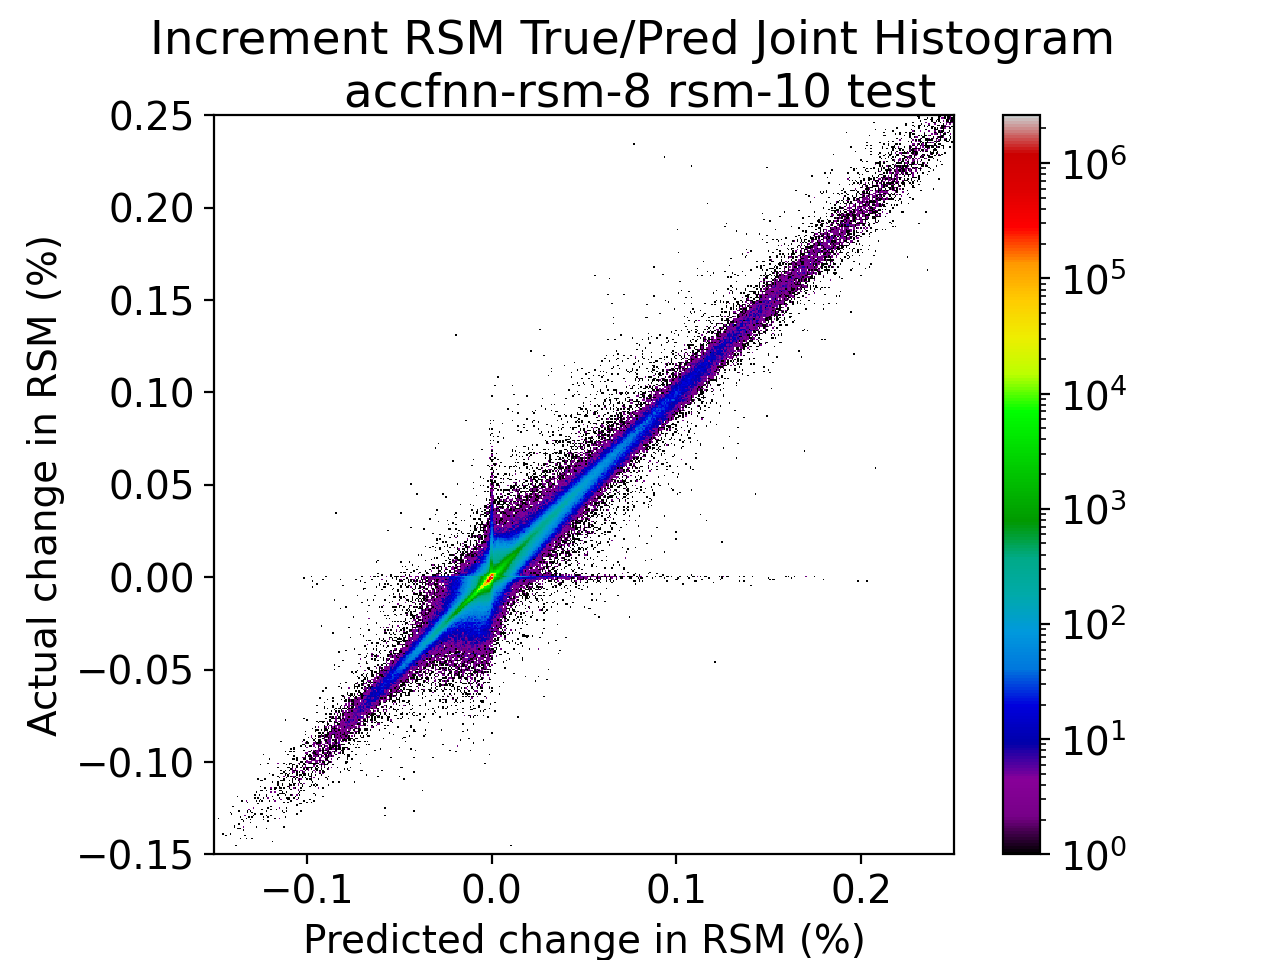
\includegraphics[width=.32\linewidth,draft=false]{figures/validation-curves/eval_test_accfnn-rsm-8_rsm-10_hist-true-pred_na.png}
    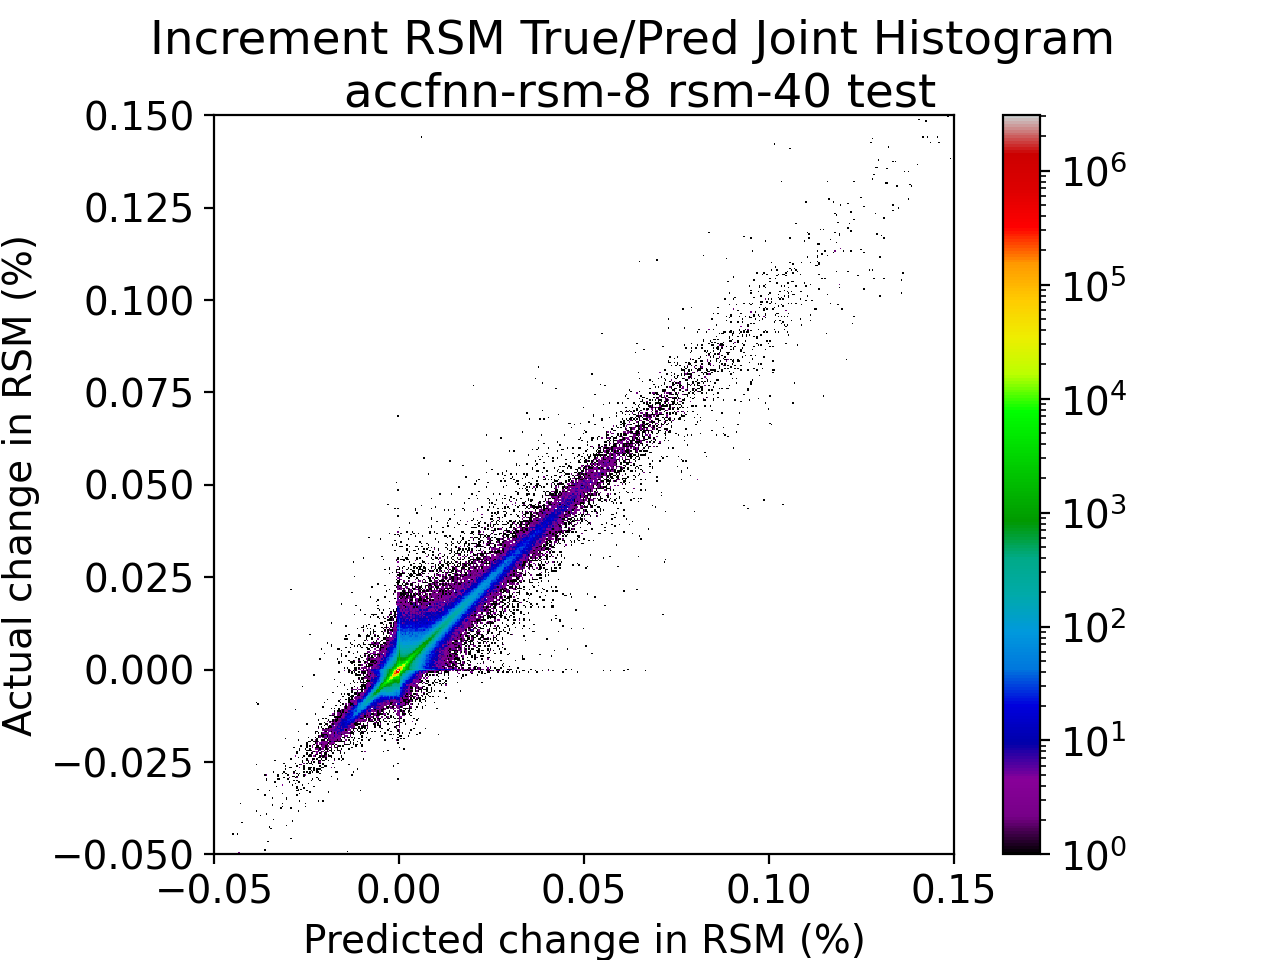
\includegraphics[width=.32\linewidth,draft=false]{figures/validation-curves/eval_test_accfnn-rsm-8_rsm-40_hist-true-pred_na.png}
    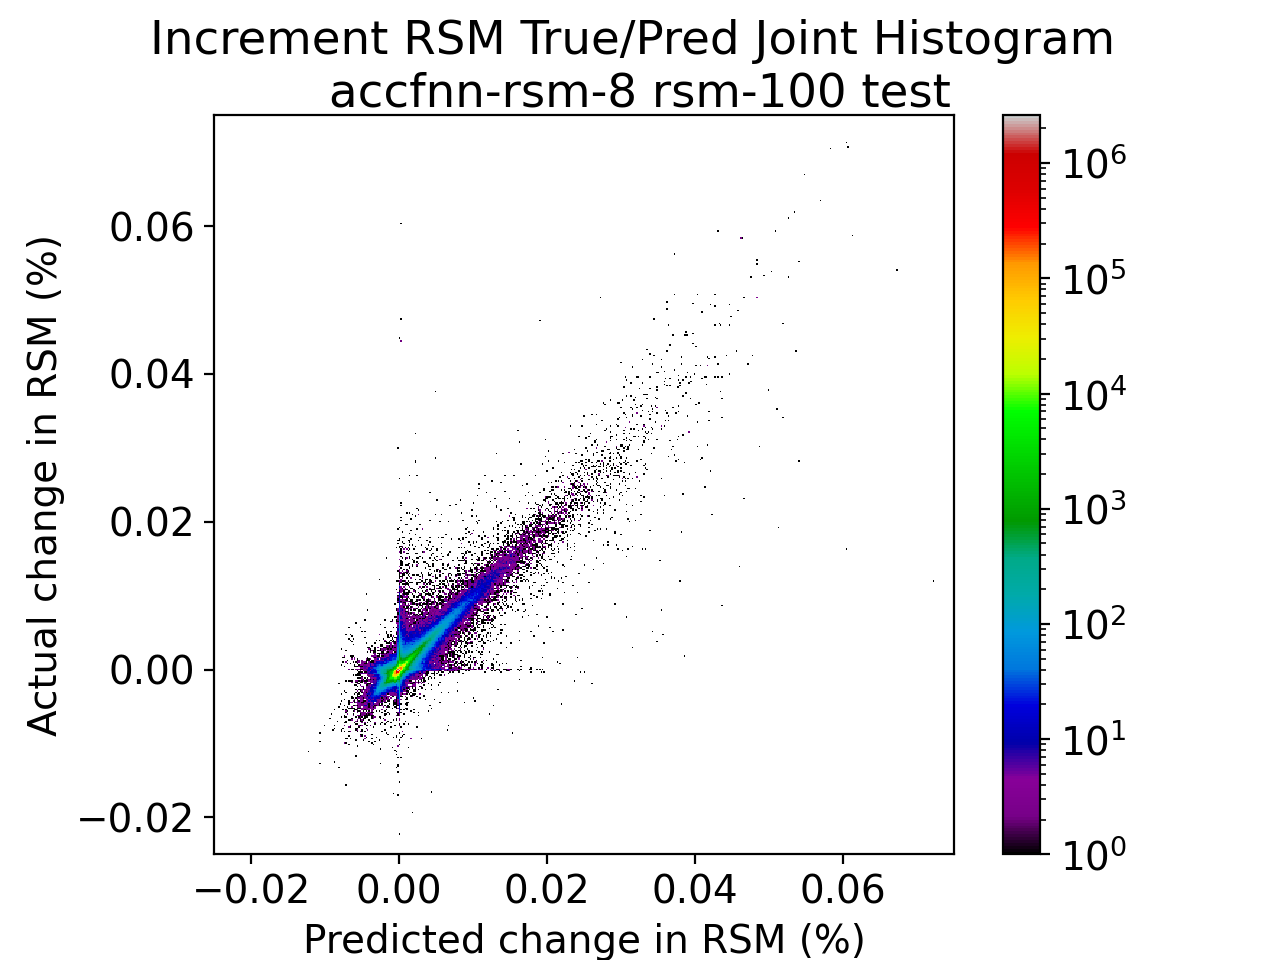
\includegraphics[width=.32\linewidth,draft=false]{figures/validation-curves/eval_test_accfnn-rsm-8_rsm-100_hist-true-pred_na.png}

    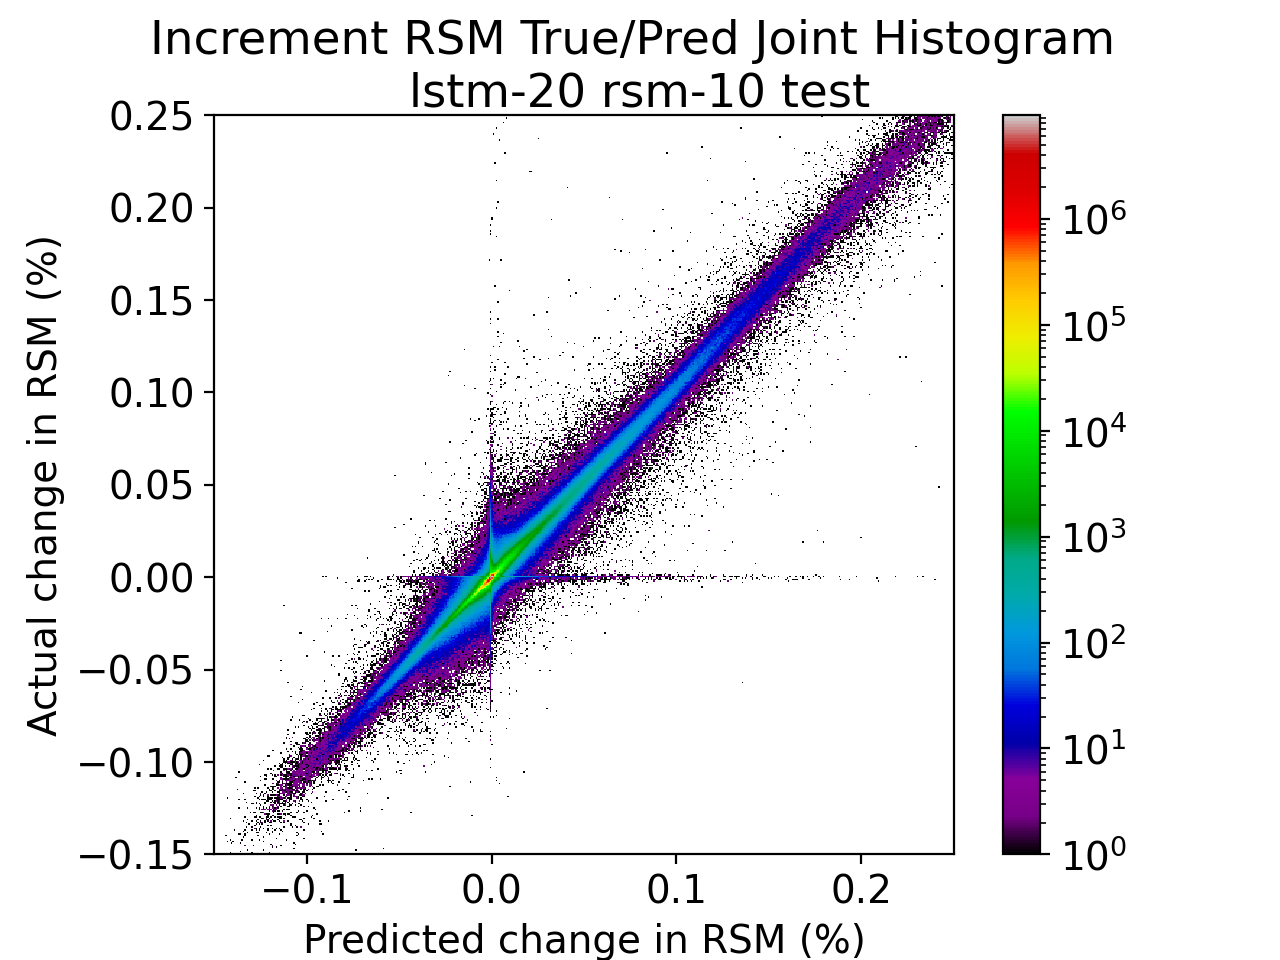
\includegraphics[width=.32\linewidth,draft=false]{figures/validation-curves/eval_test_lstm-20_rsm-10_hist-true-pred_na.png}
    \includegraphics[width=.32\linewidth,draft=false]{figures/validation-curves/eval_test_lstm-20_rsm-40_hist-true-pred_na.png}
    \includegraphics[width=.32\linewidth,draft=false]{figures/validation-curves/eval_test_lstm-20_rsm-100_hist-true-pred_na.png}

    \includegraphics[width=.32\linewidth,draft=false]{figures/validation-curves/eval_test_lstm-rsm-9_rsm-10_hist-true-pred_na.png}
    \includegraphics[width=.32\linewidth,draft=false]{figures/validation-curves/eval_test_lstm-rsm-9_rsm-40_hist-true-pred_na.png}
    \includegraphics[width=.32\linewidth,draft=false]{figures/validation-curves/eval_test_lstm-rsm-9_rsm-100_hist-true-pred_na.png}

    %\includegraphics[width=.32\linewidth,draft=false]{figures/validation-curves/eval_test_acclstm-rsm-4_rsm-10_hist-true-pred_na.png}
    %\includegraphics[width=.32\linewidth,draft=false]{figures/validation-curves/eval_test_acclstm-rsm-4_rsm-40_hist-true-pred_na.png}
    %\includegraphics[width=.32\linewidth,draft=false]{figures/validation-curves/eval_test_acclstm-rsm-4_rsm-100_hist-true-pred_na.png}

    \caption{Heatmaps of true/predicted joint histograms for each of the top 3 soil layers, as predicted by the best models from each category.}
    \label{best-validation}
\end{figure}

\begin{figure}[hp!]
    \centering

    \includegraphics[width=.32\linewidth,draft=false]{figures/static-combos/eval_test_accfnn-rsm-8_rsm-10_static-combos_abs-err_state.png}
    \includegraphics[width=.32\linewidth,draft=false]{figures/static-combos/eval_test_accfnn-rsm-8_rsm-40_static-combos_abs-err_state.png}
    \includegraphics[width=.32\linewidth,draft=false]{figures/static-combos/eval_test_accfnn-rsm-8_rsm-100_static-combos_abs-err_state.png}

    \includegraphics[width=.32\linewidth,draft=false]{figures/static-combos/eval_test_lstm-20_rsm-10_static-combos_abs-err_state.png}
    \includegraphics[width=.32\linewidth,draft=false]{figures/static-combos/eval_test_lstm-20_rsm-40_static-combos_abs-err_state.png}
    \includegraphics[width=.32\linewidth,draft=false]{figures/static-combos/eval_test_lstm-20_rsm-100_static-combos_abs-err_state.png}

    \includegraphics[width=.32\linewidth,draft=false]{figures/static-combos/eval_test_lstm-rsm-9_rsm-10_static-combos_abs-err_state.png}
    \includegraphics[width=.32\linewidth,draft=false]{figures/static-combos/eval_test_lstm-rsm-9_rsm-40_static-combos_abs-err_state.png}
    \includegraphics[width=.32\linewidth,draft=false]{figures/static-combos/eval_test_lstm-rsm-9_rsm-100_static-combos_abs-err_state.png}

    %\includegraphics[width=.32\linewidth,draft=false]{figures/static-combos/eval_test_acclstm-rsm-4_rsm-10_static-combos_abs-err_state.png}
    %\includegraphics[width=.32\linewidth,draft=false]{figures/static-combos/eval_test_acclstm-rsm-4_rsm-40_static-combos_abs-err_state.png}
    %\includegraphics[width=.32\linewidth,draft=false]{figures/static-combos/eval_test_acclstm-rsm-4_rsm-100_static-combos_abs-err_state.png}

    \caption{Absolute error of best models' state from each category with respect to static categorical parameter combinations.}
    \label{best-static-abserr}
\end{figure}

\begin{figure}[hp!]
    \centering

    \includegraphics[width=.32\linewidth,draft=false]{figures/static-combos/eval_test_accfnn-rsm-8_rsm-10_static-combos_bias_state.png}
    \includegraphics[width=.32\linewidth,draft=false]{figures/static-combos/eval_test_accfnn-rsm-8_rsm-40_static-combos_bias_state.png}
    \includegraphics[width=.32\linewidth,draft=false]{figures/static-combos/eval_test_accfnn-rsm-8_rsm-100_static-combos_bias_state.png}

    \includegraphics[width=.32\linewidth,draft=false]{figures/static-combos/eval_test_lstm-20_rsm-10_static-combos_bias_state.png}
    \includegraphics[width=.32\linewidth,draft=false]{figures/static-combos/eval_test_lstm-20_rsm-40_static-combos_bias_state.png}
    \includegraphics[width=.32\linewidth,draft=false]{figures/static-combos/eval_test_lstm-20_rsm-100_static-combos_bias_state.png}

    \includegraphics[width=.32\linewidth,draft=false]{figures/static-combos/eval_test_lstm-rsm-9_rsm-10_static-combos_bias_state.png}
    \includegraphics[width=.32\linewidth,draft=false]{figures/static-combos/eval_test_lstm-rsm-9_rsm-40_static-combos_bias_state.png}
    \includegraphics[width=.32\linewidth,draft=false]{figures/static-combos/eval_test_lstm-rsm-9_rsm-100_static-combos_bias_state.png}

    %\includegraphics[width=.32\linewidth,draft=false]{figures/static-combos/eval_test_acclstm-rsm-4_rsm-10_static-combos_bias_state.png}
    %\includegraphics[width=.32\linewidth,draft=false]{figures/static-combos/eval_test_acclstm-rsm-4_rsm-40_static-combos_bias_state.png}
    %\includegraphics[width=.32\linewidth,draft=false]{figures/static-combos/eval_test_acclstm-rsm-4_rsm-100_static-combos_bias_state.png}

    \caption{Bias of best models' state from each category with respect to static categorical parameter combinations.}
    \label{best-static-bias}
\end{figure}

\section{Spatial, Temporal, and Situational Evaluation}

\begin{figure}[hp!]
    \centering

    \includegraphics[width=.48\linewidth,draft=false]{figures/grid-eval_lstm-rsm-9_full/eval-grid_full_lstm-rsm-9_rsm-10_spatial-stats_abs-err_state-err-abs-mean.png}
    \includegraphics[width=.48\linewidth,draft=false]{figures/grid-eval_lstm-rsm-9_full/eval-grid_full_lstm-rsm-9_rsm-10_spatial-stats_abs-err_state-err-abs-stdev.png}

    \includegraphics[width=.48\linewidth,draft=false]{figures/grid-eval_lstm-rsm-9_full/eval-grid_full_lstm-rsm-9_rsm-10_spatial-stats_bias_state-err-bias-mean.png}
    %\includegraphics[width=.48\linewidth,draft=false]{figures/grid-eval_lstm-rsm-9_full/eval-grid_full_lstm-rsm-9_rsm-10_spatial-stats_bias_state-err-bias-stdev.png}

    \caption{Gridded MAE, bias in state, and the standard deviation of MAE, for 0-10cm layer}
    \label{lstm-rsm-9-grid-rsm-10}
\end{figure}

\begin{figure}[hp!]
    \centering

    \includegraphics[width=.48\linewidth,draft=false]{figures/grid-eval_lstm-rsm-9_full/eval-grid_full_lstm-rsm-9_rsm-40_spatial-stats_abs-err_state-err-abs-mean.png}
    \includegraphics[width=.48\linewidth,draft=false]{figures/grid-eval_lstm-rsm-9_full/eval-grid_full_lstm-rsm-9_rsm-40_spatial-stats_abs-err_state-err-abs-stdev.png}

    \includegraphics[width=.48\linewidth,draft=false]{figures/grid-eval_lstm-rsm-9_full/eval-grid_full_lstm-rsm-9_rsm-40_spatial-stats_bias_state-err-bias-mean.png}
    %\includegraphics[width=.48\linewidth,draft=false]{figures/grid-eval_lstm-rsm-9_full/eval-grid_full_lstm-rsm-9_rsm-40_spatial-stats_bias_state-err-bias-stdev.png}

    \caption{Gridded MAE, bias in state, and the standard deviation of MAE, for 10-40cm layer}
    \label{lstm-rsm-9-grid-rsm-40}
\end{figure}

\begin{figure}[hp!]
    \centering

    \includegraphics[width=.48\linewidth,draft=false]{figures/grid-eval_lstm-rsm-9_full/eval-grid_full_lstm-rsm-9_rsm-100_spatial-stats_abs-err_state-err-abs-mean.png}
    \includegraphics[width=.48\linewidth,draft=false]{figures/grid-eval_lstm-rsm-9_full/eval-grid_full_lstm-rsm-9_rsm-100_spatial-stats_abs-err_state-err-abs-stdev.png}

    \includegraphics[width=.48\linewidth,draft=false]{figures/grid-eval_lstm-rsm-9_full/eval-grid_full_lstm-rsm-9_rsm-100_spatial-stats_bias_state-err-bias-mean.png}
    %\includegraphics[width=.48\linewidth,draft=false]{figures/grid-eval_lstm-rsm-9_full/eval-grid_full_lstm-rsm-9_rsm-100_spatial-stats_bias_state-err-bias-stdev.png}

    \caption{Gridded MAE, bias in state, and the standard deviation of MAE for 40-100cm layer}
    \label{lstm-rsm-9-grid-rsm-100}
\end{figure}

\begin{figure}[hp!]
    \centering

    \includegraphics[width=.96\linewidth,draft=false]{figures/grid-eval_lstm-rsm-9_full/eval-grid_full_lstm-rsm-9_rsm-10_hist-humidity-temp_abs-err.png}
    \includegraphics[width=.96\linewidth,draft=false]{figures/grid-eval_lstm-rsm-9_full/eval-grid_full_lstm-rsm-9_rsm-10_hist-humidity-temp_bias.png}

    \caption{Joint histogram of humidity and temperature forcings, with mean absolute error (top) and error bias (bottom) plotted within corresponding bins.}
    \label{lstm-rsm-9-hthist}
\end{figure}

\begin{figure}[hp!]
    \centering

    \includegraphics[width=.96\linewidth,draft=false]{figures/grid-eval_lstm-rsm-9_full/eval-grid_full_lstm-rsm-9_rsm-10_hist-state-increment_abs-err.png}
    \includegraphics[width=.96\linewidth,draft=false]{figures/grid-eval_lstm-rsm-9_full/eval-grid_full_lstm-rsm-9_rsm-10_hist-state-increment_bias.png}

    \caption{Joint histogram of total RSM and increment change of RSM in the 0-10cm layer, with mean absolute error (top) and error bias (bottom) plotted within corresponding bins.}
    \label{lstm-rsm-9-sihist-rsm-10}
\end{figure}

\begin{figure}[hp!]
    \centering

    \includegraphics[width=.96\linewidth,draft=false]{figures/grid-eval_lstm-rsm-9_full/eval-grid_full_lstm-rsm-9_rsm-40_hist-state-increment_abs-err.png}
    \includegraphics[width=.96\linewidth,draft=false]{figures/grid-eval_lstm-rsm-9_full/eval-grid_full_lstm-rsm-9_rsm-40_hist-state-increment_bias.png}

    \caption{Joint histogram of total RSM and increment change of RSM in the 10-40cm layer, with mean absolute error (top) and error bias (bottom) plotted within corresponding bins.}
    \label{lstm-rsm-9-sihist-rsm-40}
\end{figure}

\begin{figure}[hp!]
    \centering

    \includegraphics[width=.96\linewidth,draft=false]{figures/grid-eval_lstm-rsm-9_full/eval-grid_full_lstm-rsm-9_rsm-100_hist-state-increment_abs-err.png}
    \includegraphics[width=.96\linewidth,draft=false]{figures/grid-eval_lstm-rsm-9_full/eval-grid_full_lstm-rsm-9_rsm-100_hist-state-increment_bias.png}

    \caption{Joint histogram of total RSM and increment change of RSM in the 40-100cm layer, with mean absolute error (top) and error bias (bottom) plotted within corresponding bins.}
    \label{lstm-rsm-9-sihist-rsm-100}
\end{figure}

\section{Parameter Variations}

\section{Case Studies}

